\documentclass[12pt,a4paper]{report}
\usepackage[utf8]{inputenc}
\usepackage[T1]{fontenc}
\usepackage{fontspec}
\usepackage{amsmath}
\usepackage{amsfonts}
\usepackage{amssymb}
\usepackage[polish]{babel}
\usepackage{graphicx}
\usepackage{amssymb}
\usepackage{bbold}
\usepackage[table,xcdraw, dvipsnames]{xcolor}
\usepackage{hhline}
\usepackage{placeins}
\usepackage[margin=0.6in]{geometry}
\usepackage{appendix}
\usepackage{caption}
\usepackage{colortbl}
\usepackage{physics}
\usepackage{float}
\usepackage{datetime}
\usepackage{makeidx}
\usepackage{hyperref}
\usepackage[normalem]{ulem}

\title{Mechanika Kwantowa R 2021/2022}
\author{Kacper Cybiński}
% \newdate{date}{28}{01}{2022}
% \date{\displaydate{date}}
\date{\today}
\makeindex
\setlength\parindent{0pt}

\addto\captionspolish{\renewcommand{\chaptername}{Lecture}}

\newcommand{\ind}[1]{{\color{blue} #1\index{#1}}}

\newcommand{\subind}[2]{{\color{blue} #1\index{#2}}}

\newcommand{\com}[1]{{\color{red} #1}}

\newcommand{\link}[2]{{\color{cyan} \href{#1}{#2}}}

\newcommand{\uwaga}[1]{{\color{violet} Uwaga:} #1}

\newcommand{\phys}{\stackrel{\text{F}}{\equiv}}

\newcommand{\E}{\mathcal{E}}

\newcommand{\R}{\mathcal{R}}

\newcommand{\T}{\mathcal{T}}

\newcommand{\HS}{\mathcal{H}}

\newcommand{\CS}{\mathcal{C}}

\newcommand{\phat}{\hat{p}}

\newcommand{\xhat}{\hat{x}}

\newcommand{\ahat}{\hat{a}}

\newcommand{\psket}[1]{\ket{\Psi(#1)}}

\newcommand{\tpsi}{\tilde{\Psi}}

\newcommand{\Id}{\mathbb{1}}

\renewcommand{\emph}{\textbf}

\newcommand{\rket}{\ket{\va{r}}}

\newcommand{\pd}[1]{\partial_{#1}}

\renewcommand{\rho}{\varrho}

\renewcommand{\phi}{\varphi}

\newcommand{\linediv}{{\color{RubineRed} \rule{\linewidth}{0.5mm}}}

\newcommand{\fft}[1]{\frac{1}{\sqrt{2\pi\hbar}} \int \dd{x} #1 e^{-\frac{ixp}{\hbar}}}

\newenvironment{lecture}[1]{\par\medskip
   \noindent\chapter{#1} \rmfamily}{\medskip}
   
\newenvironment{emph_box}[1]
    {\begin{center}\color{BrickRed}
    \begin{tabular}{|p{0.9\textwidth}|}
    \hline
    \begin{center} \color{Dandelion}{\textbf{#1}} \end{center}
    \begin{center}
    }
    {
    \end{center}
    \\\\\hline
    \end{tabular} 
    \end{center}
    \color{black}
    }

\DeclareMathOperator*{\SumInt}{%
\mathchoice%
  {\ooalign{$\displaystyle\sum$\cr\hidewidth$\displaystyle\int$\hidewidth\cr}}
  {\ooalign{\raisebox{.14\height}{\scalebox{.7}{$\textstyle\sum$}}\cr\hidewidth$\textstyle\int$\hidewidth\cr}}
  {\ooalign{\raisebox{.2\height}{\scalebox{.6}{$\scriptstyle\sum$}}\cr$\scriptstyle\int$\cr}}
  {\ooalign{\raisebox{.2\height}{\scalebox{.6}{$\scriptstyle\sum$}}\cr$\scriptstyle\int$\cr}}
}

\begin{document}

\maketitle

\chapter*{Organizacja wykładu}
\begin{enumerate}
    \item Dwa kolokwia - po 30 pkt
    \item Egzamin - 40 pkt
\end{enumerate}
Łącznie 100 pkt, progi punktowe:
\[45-55 = 3, 55-65 = 3.5, 65-75=4, 75-85=4.5, 85-95 = 5, 95-100=5!\]

Egzamin ustny (zmiana oceny co najwyżej o 0.5)

Serie domowe dobrowolne (ale na pewno pomogą napisać dobrze kolokwia!)

{\color{blue} \link{https://kampus-student2.ckc.uw.edu.pl/course/view.php?id=9707}{Strona wykładu}}


Polecane podręczniki:
\begin{itemize}
    \item L. Schiff \textit{Mechanika Kwantowa (obszerna)}
    \item R. Liboff \textit{Wprowadzenie do Mechaniki Kwantowej} \textit{(mniej obszerna)}
    \item L. Susskind \textit{Quantum Mechanics (Do ogarnięcia koncepcyjnego)}
\end{itemize}

\begin{lecture}{Krótka historia fizyki i wstęp do kwantów}
    \section{Krótka historia fizyki}
    \begin{itemize}
        \item {\bf Arystoteles} - Jeden absolutny układ odniesienia, więc nie ma sensu pojęcie \textit{obserwatora}
        \item {\bf Newton} - Ciała, a więc i układy odniesienia (obserwatorzy inercjalni) są liczne, oraz mogą się poruszać między sobą. Siła, czas, przestrzeń są wciąż pojęciami absolutnymi.
        \item {\bf Teoria względności} - Ruch, czas, przestrzeń, masa są zależne od obserwatora. Obserwator nie musi być inercjalny. Mówimy o {\it Uoperacyjnieniu pojęć zasadniczych}.
        \item {\bf Teoria Kwantowa} - Okazuje się, że cały zestaw wielkości fizycznych służących do opisu świata zależy od tego jaki jest kontekst pomiarowy, tj. od relacji obserwatora z innymi elementami otaczającego go świata. {\it Czyli po raz pierwszy uwzględniamy fakt, że opisujemy wszechświat w którym sami istniejemy, czyli opisujemy ten układ {\bf od środka}}.
    \end{itemize}
    \link{http://studenci.fuw.edu.pl/~kc427902/Prezentacje_Kwanty/HisotriaFIzykiWitkacy.pdf}{Prezentacja o historii fizyki wg Witkacego}
    
    
    \section{Hipoteza Kwantu}
    Co doprowadziło do wniosków, że energię trzeba skwantować?
    \subsection{Ciało Doskonale Czarne}
    Paradoks polegał na tym, że z ciała doskonale czarnego powinniśmy mieć zabójcze promieniowanie gamma itp, a go nie było IRL. And here comes the {\it Max Planck}.\\
    Planck zapostulował, że przekaz energii odbywa się za pomocą całkowitych wartośći (\ind{Kwant Energii})
    Zdefiniował to jako:
    \begin{equation}
        E = h \cdot \nu = \hbar \cdot \omega
        \label{eq:lec_1:E_planck}
    \end{equation}
    \[\hbar = \frac{h}{2 \pi}, \omega = 2 \pi \nu\]
    gdzie h - \subind{Stała Plancka}{Stała!Plancka}, $h = 6.2626070150 \cdot 10^{-34} J\cdot s$, $\nu$ - częstotliwość promieniowania 
    \begin{figure}[!ht]
        \centering
        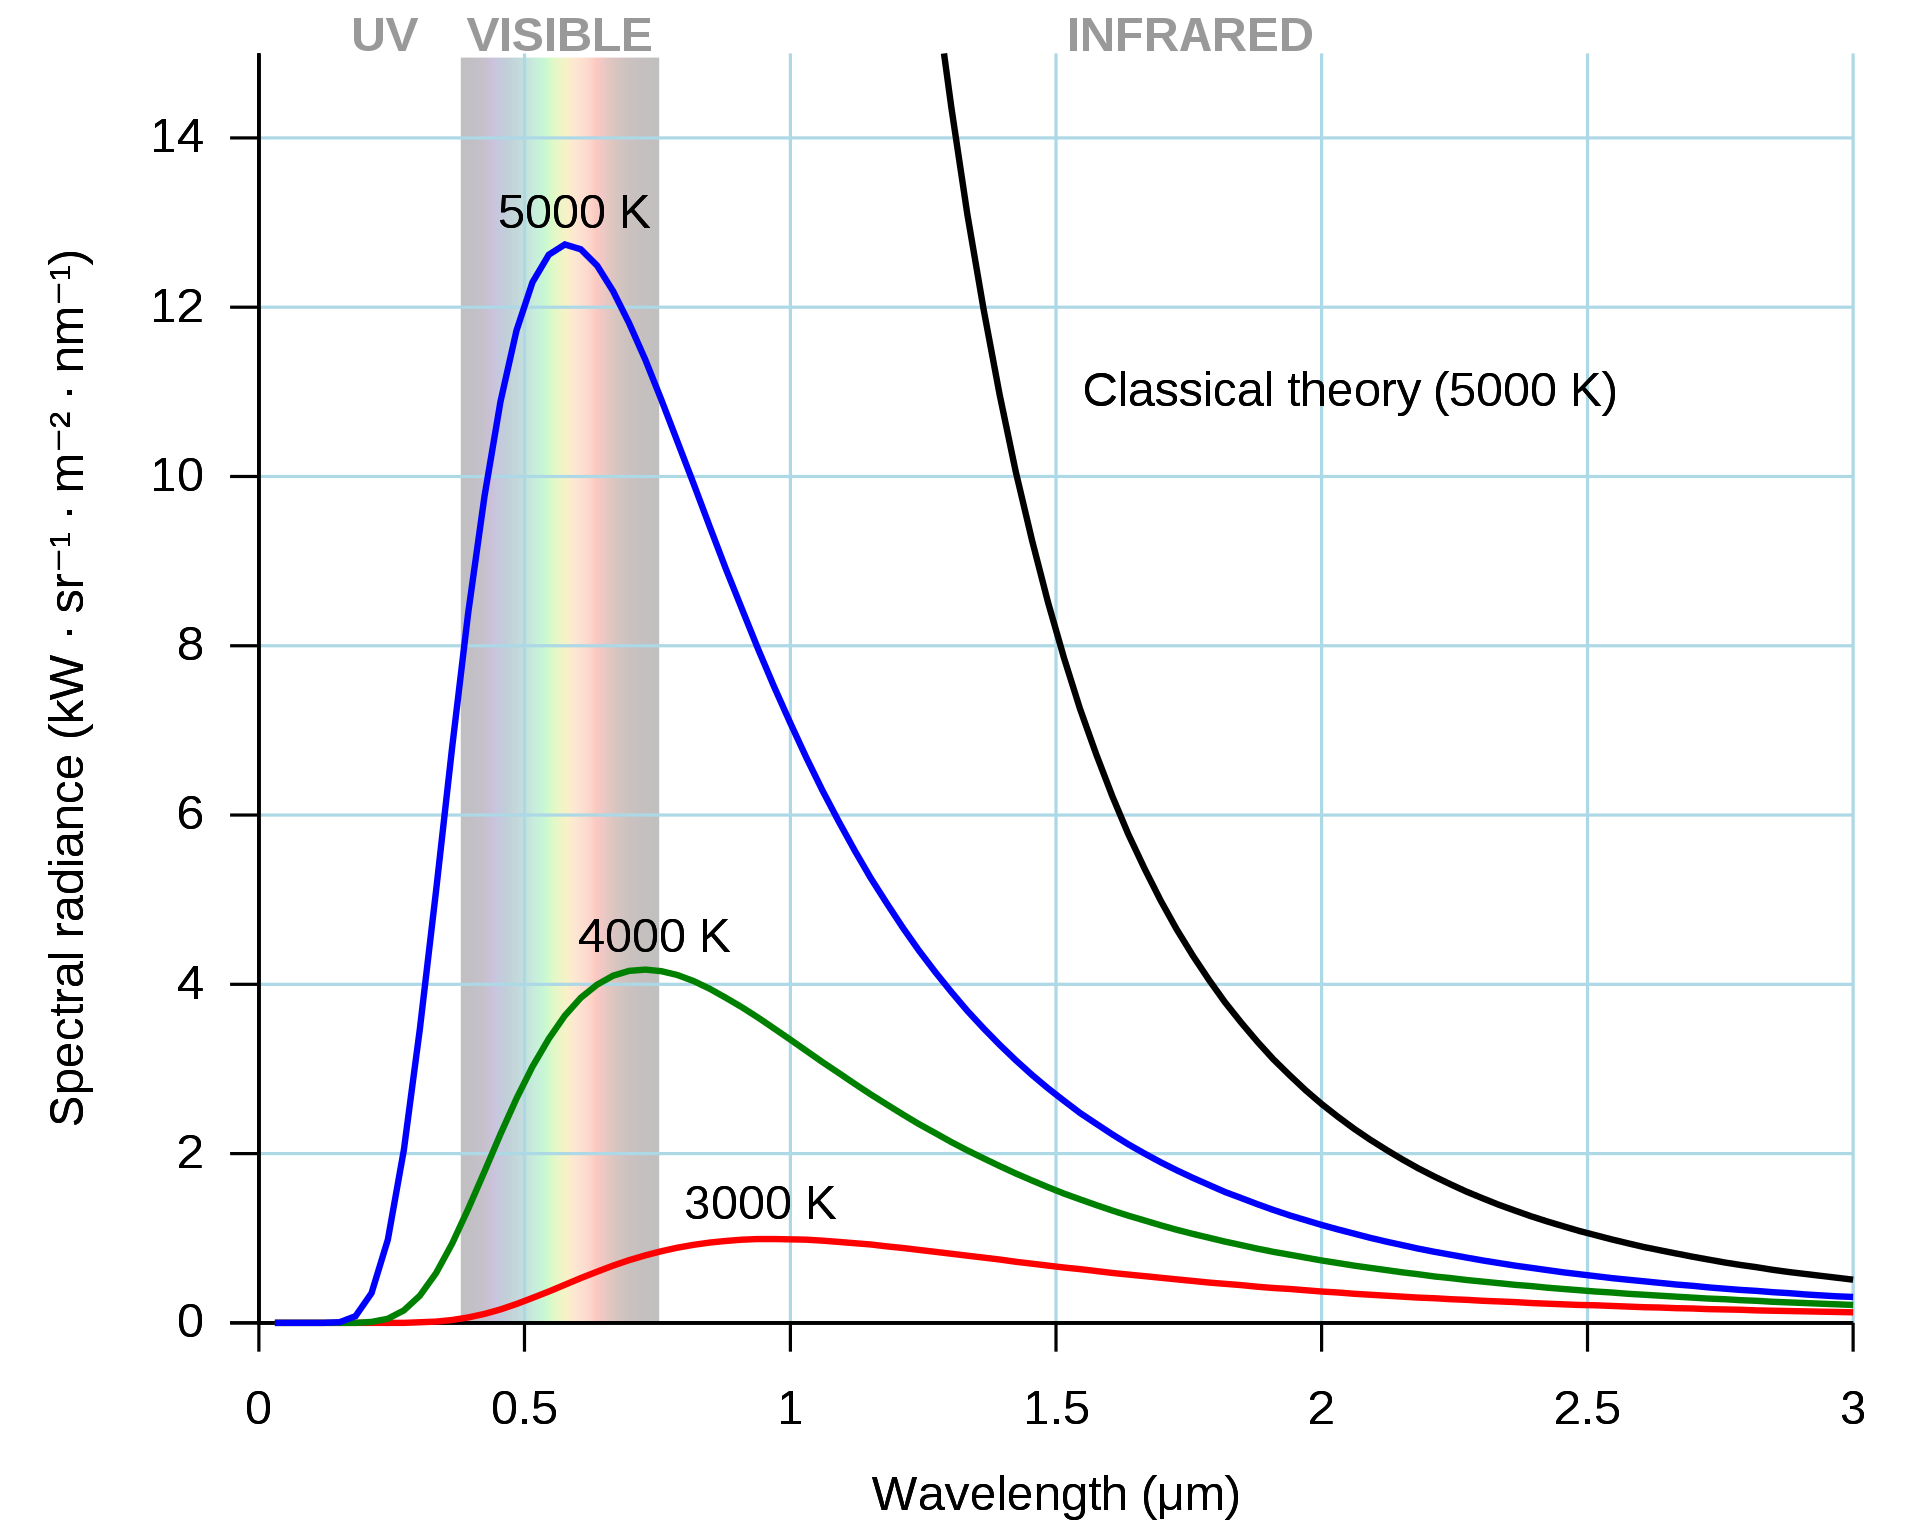
\includegraphics[width=\linewidth]{Wyk_1_Rys_5.png}
        \caption{Wykres promieniowania ciała doskonale czarnego}
        \label{fig:lec_1:cialo_doskonale_czarne}
    \end{figure}
    
    \begin{figure}[!ht]
        \centering
        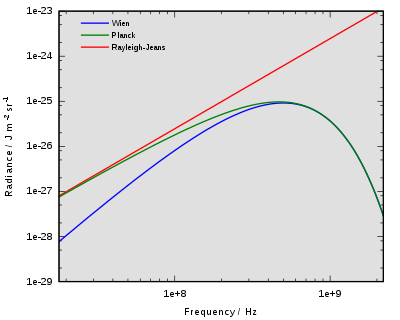
\includegraphics[width=\linewidth]{Wyk_1_Rys_6.png}
        \caption{Porównanie hipotezy Plancka z prawem Rayleigha-Jeansa i rozkładem Wiena. Further reading o 'Katastrofie w nadfiolecie'  na \link{https://pl.wikipedia.org/wiki/Ciało_doskonale_czarne}{Wikipedii o ciele doskonale czarnym}}
        \label{fig:lec_1:cialo_doskonale_czarne_porownanie}
    \end{figure}
    
    \subsection{Efekt Fotoelektryczny}
    \subsection{Analiza pól EM}
    Analiza pól $\E$ i B w odniesieniu do sześcianu z przewodnika prowadzi do wniosku, że energia "porcji promieniowania" transformuje się jak 
    \[\frac{\E'}{\E} = \frac{\sqrt{1 - \frac{u}{c}}}{\sqrt{1 + \frac{u}{c}}}\]
    gdzie $u$ - promieniowanie.
    Transformuje się to analogicznie do częstotliwości w efekcie Dopplera $\implies E \sim \nu$
    \\
    Rozkład energii będzie nam opisywać \ind{Rozkład Boltzmanna}, czyli rozkład prawdopodobieństwa zaobserwowania stanu Energetycznego, dany wzorem:
    \[p(E_i) \sim e^{-\frac{E_i}{k T}}\]
    co w przypadku rozkładu ciągłego daje nam zasadę ekwipartycji, ale dla dużych wartości energii się rozbiega z doświadczenie.
    
    \section{Skutki skwantowania energii}
    Przede wszystkim skutkiem jest \ind{indeterminizm}.\\
    
    \begin{figure}[!ht]
        \centering
        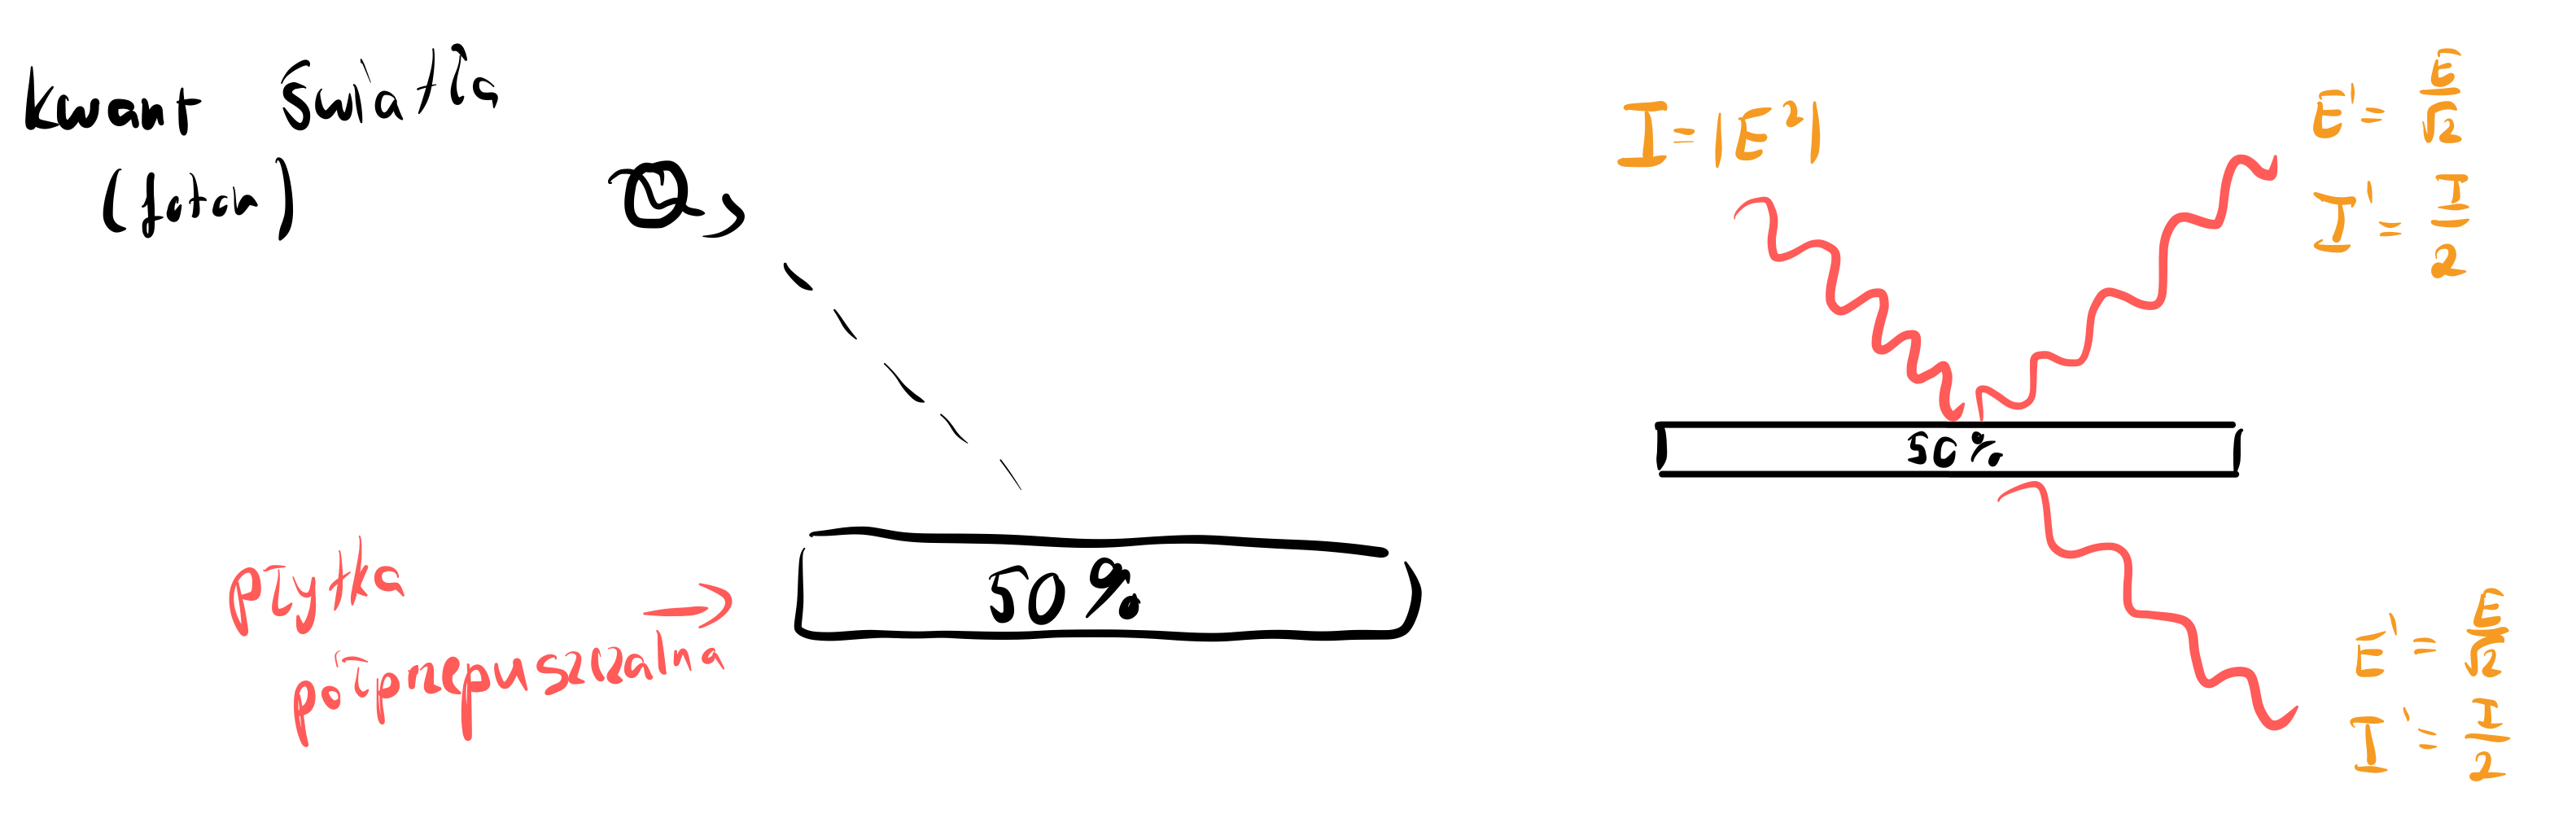
\includegraphics[width=\linewidth]{Wyk_1_Rys_1.jpeg}
        \caption{Demonstracja działania płytki półprzepusczalnej.}
        \label{fig:lec_1:plytka_polprzepuszczalna}
    \end{figure}
    
    \ind{Teoria parametrów ukrytych} - Teoria, że w kwantach energii występują nierejestrowane przez nas parametry, które jednakowoż zawsze determinują rozróżnienie kwantów energii. Parafrazując Drażana, dodawanie fotonom(kwantom) "włosów", "ogonów" itp - elementów rozróżniających je.\\
    
    Jeśli jednak nie chcemy dodawać fotonom 'włosów', ani 'ogonów' i chcielibysmy, żeby wszystkie fotony były "identyczne" to aby odtworzyć zachowanie klasyczne w granicy (podział natężenia 50\%), to musimy uznać, ze foton zachowuje się niedeterministycznie, tj. wprowadzić element probabilistyczny. Wtedy z prawdopodobieństwem 50\% każdy foton przechodzi lub odbija się.
    
    \begin{figure}[!ht]
        \centering
        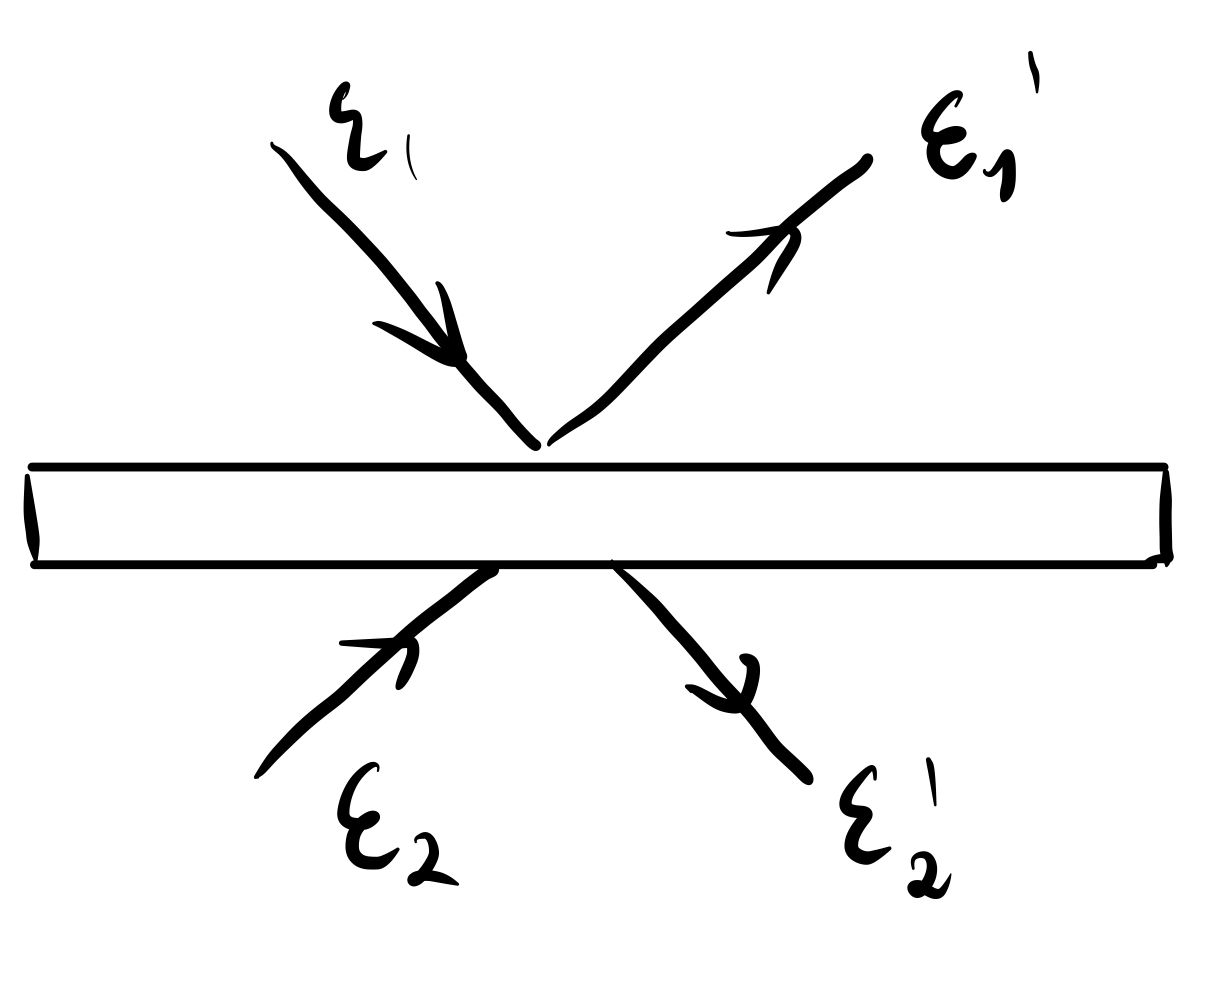
\includegraphics[width=0.6\linewidth]{Wyk_1_Rys_2.jpeg}
        \caption{Demonstracja działania płytki światłodzielącej ({\it Beam Splitter}).}
        \label{fig:lec_1:beam_splitter}
    \end{figure}
    
    Kiedy patrzymy na płytkę światłodzielącą (Rysunek \ref{fig:lec_1:beam_splitter}), to możemy przedstawiać bieg promienia w niej jako superpozycję fal (zapis macierzowy).
    \[\mqty[\E_1' \\ \E_2'] = B \mqty[\E_1 \\ \E_2] \implies \mqty[\R_1 & \T_2 \\ \T_1 & \R_2]\]
    Gdzie $\E_1' = \R1\E_1 + \T_2\E_2$. Chcemy, żeby \emph{energia była zachowana} \[\implies \vqty{\E_1}^2 + \vqty{\E_2}^2 = \vqty{\E_1'}^2 + \vqty{\E_2'}^2\]
    Co możemy też tłumaczyć jako zachowanie długości wektora $ \mqty[\E_1' \\ \E_2']$, czyli macierz $B$ jest macierzą \emph{Unitarną}, tj. $B\cdot B^\dag = 1$. 
    
    \[
        B B^\dag = \mqty[\R_1^\ast & \T_1^\ast \\ 
        \T_2^\ast & \R_2^\ast] 
        \cdot 
        \mqty[\R_1 & \T_2 \\ \T_1 & \R_2] = 
        \mqty[\vqty{\R_1}^2 + \vqty{\T_1}^2 & \R_1^\ast\T_2 + \T_1^\ast R_2 \\ 
        \R_1\T_2^\ast + \T_1 R_2^\ast & \vqty{\R_2}^2 + \vqty{\T_2}^2] = 
        \mqty[1 & 0 \\ 0 & 1]
    \]
    
    Wynika stąd, że $\vqty{\R_1}^2 = \vqty{\R_2}^2 = R$ - współczynnik odbicia natężenia, a $\vqty{\T_1}^2 = \vqty{\T_2}^2 = T$ - współczynnik transmisji natężenia, gdzie $R + T = 1$.
    
    W związku z tym też ogólnie mówiąc np.$ B = \mqty[\sqrt{R} & \sqrt{T} \\ -\sqrt{T} & \sqrt{R}]$, a $B_{50\%} = \frac{1}{2} \mqty[1 & 1 \\ -1 & 1]$. Tj. $B \in \mathcal{U}(2)$
    
    \section{Superpozycja}
    
    Pokażemy zjawisko interferencji w sensie kwantowym patrząc na kanoniczny przykład - \ind{Interferometr Macha-Zehndera}, widoczny na Rysunku \ref{fig:lec_1:interferometer}. Rozpatrujemy od teraz falę padającą postaci $\mqty[\E \\ 0]$.
    
    \begin{figure}[!ht]
        \centering
        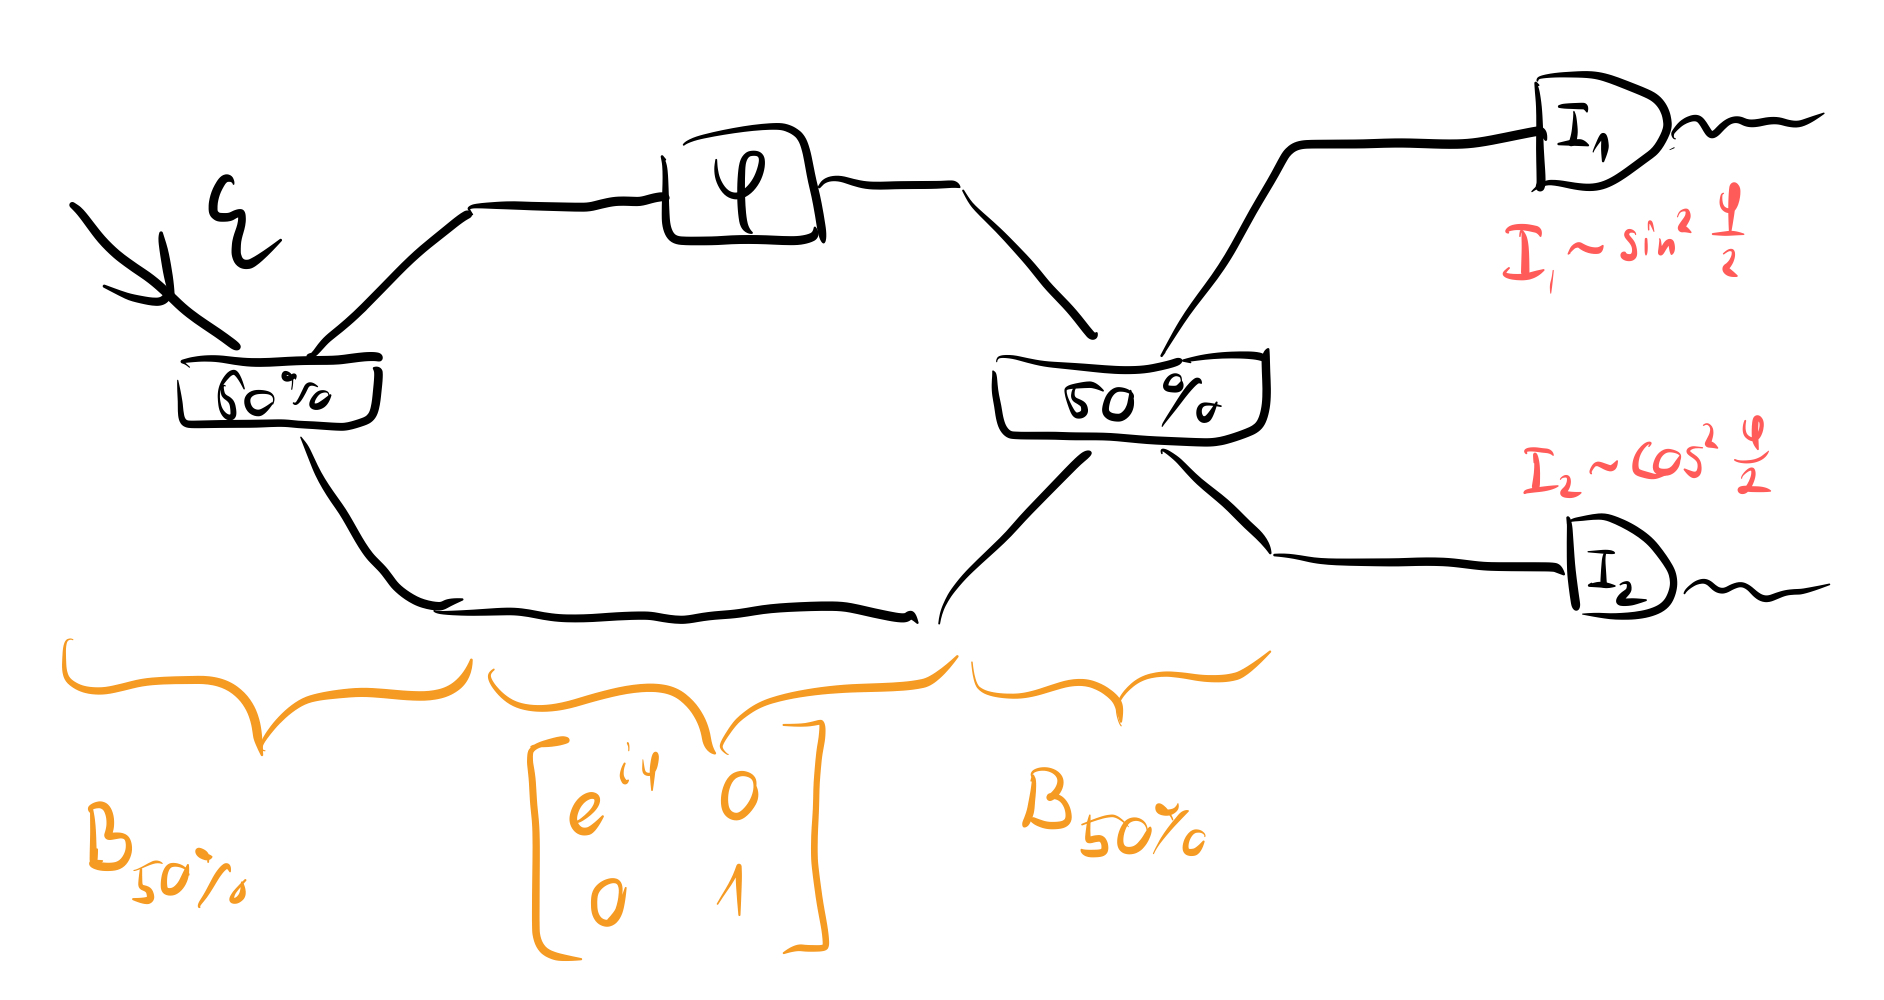
\includegraphics[width=0.8\linewidth]{Wyk_1_Rys_3.jpeg}
        \caption{Schemat konstrukcji Interferometru Macha-Zehndera wraz z podpisem macierzami Jonesa}
        \label{fig:lec_1:interferometer}
    \end{figure}
    
    \begin{figure}[!ht]
        \centering
        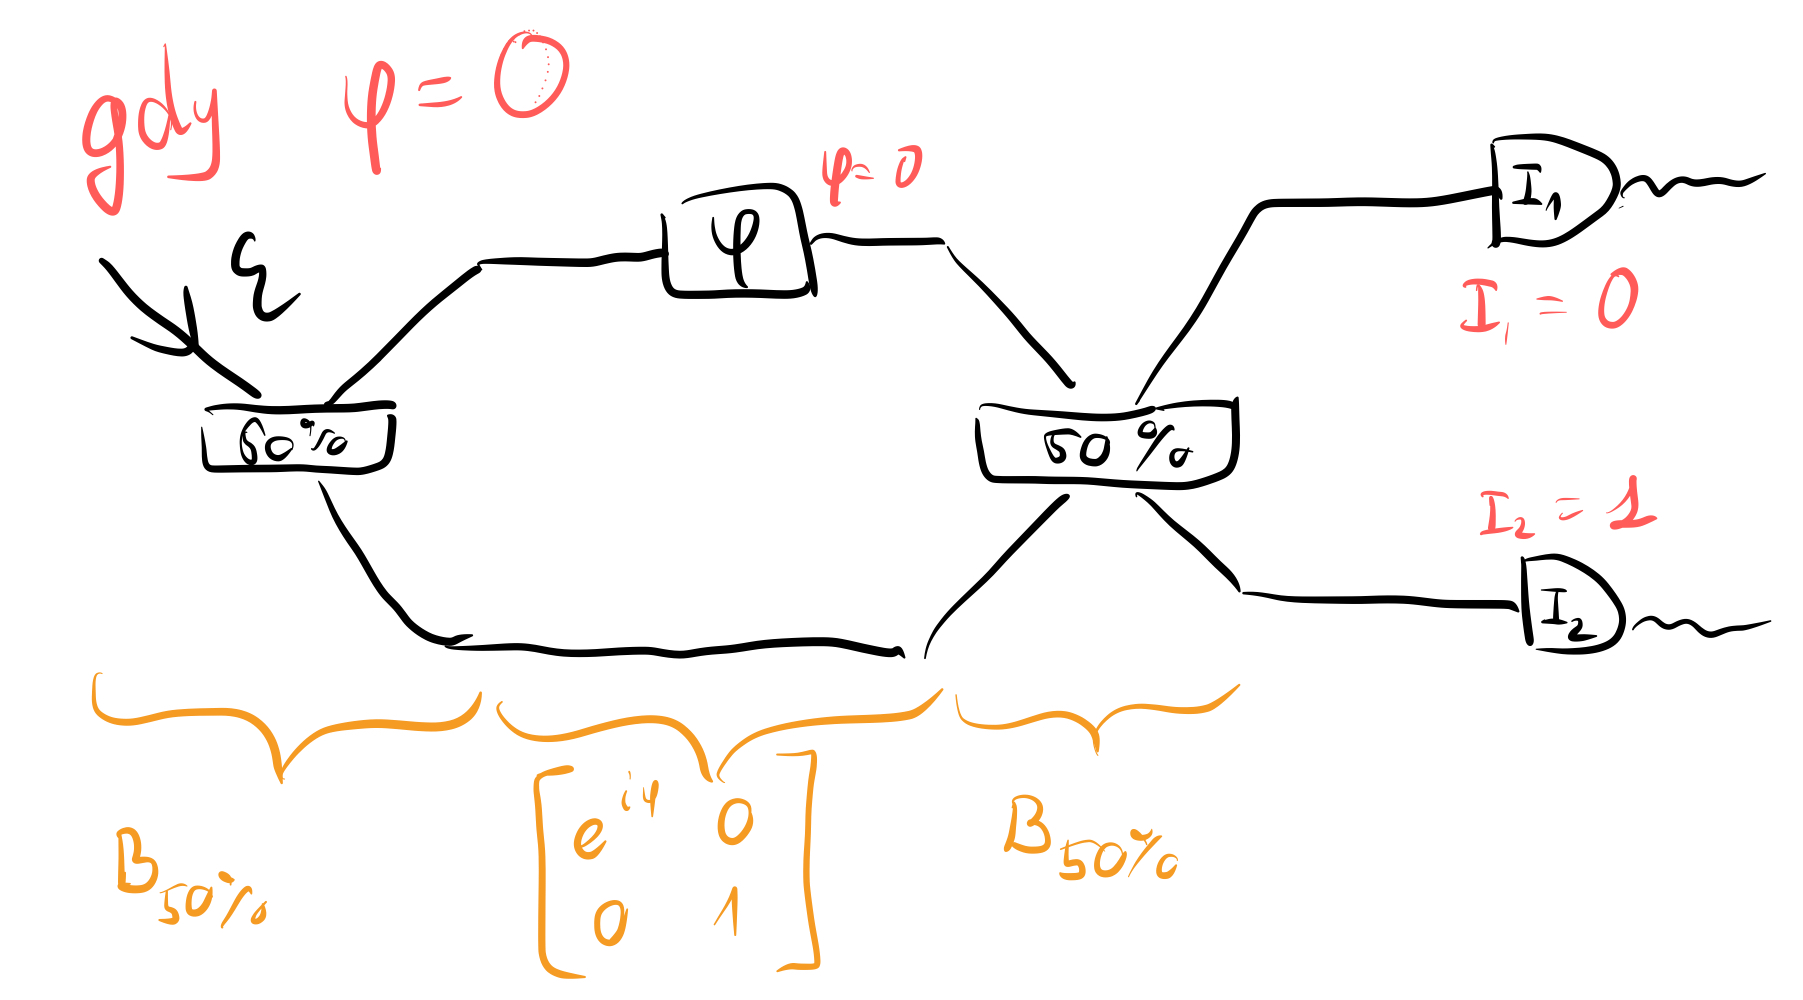
\includegraphics[width=0.8\linewidth]{Wyk_1_Rys_4.jpeg}
        \caption{Schemat konstrukcji Interferometru Macha-Zehndera wraz z podpisem macierzami Jonesa w przypadku zerowej zmiany fazy, tj. w szczególności dla jednego fotonu}
        \label{fig:lec_1:interferometer_phi_0}
    \end{figure}
    
    Teraz aby zrozumieć jak w takim układzie zachowuje się foton musimy odejść od klasycznego myślenia, że leci on jakąś drogą, a musimy przejść do myślenia o jego drodze jako \emph{nieokreślonej}, tj. do momentu wykonania pomiaru (wejścia w interakcję z nim) podąża on jednocześnie wszyskimi możliwymi dla siebie trajektoriami, tym samym przyjmując właściwości falowe. Da to efekt jak ten widoczny na Rysunku \ref{fig:lec_1:interferometer_phi_0}.
    
    Od teraz ten stan 'obierania wszystkich możliwości na raz' przez foton będziemy określać jako \subind{stan fotonu}{Stan!fotonu} oznaczany $\ket{\Psi}$. Tłumaczy się to na funkcję gęstości prawdopodobieństwa znalezienia fotonu w jego możliwych trajektoriach.
    
    W szczególności w opisywanym wyżej przypadku stan $\ket{\Psi}$ będzie opisywany przez \emph{superpozycję} stanów 1 i 2 odpowiadających pójściem drogą odpowiednio górną i dolną, tj. $\ket{\Psi} = \mqty[\Psi_1 \\ \Psi_2]$ gdzie $\Psi_i$ - aplituda prawdopodobieństwa obrania ścieżki $i$, a $p_i = \qty|\Psi_i|^2$ - prawdopodobieństwo, że foton leci i-tą trajektorią.
    
    \begin{equation}
        \ket{\Psi} = \Psi_1\ket{1} \oplus \Psi_2 \ket{2}
        \label{eq:lec_1:superpozycja}
    \end{equation}
    
    Gdzie znakiem $\oplus$ oznaczamy dodawanie fal. Ta operacja to \ind{Superpozycja}. Warto też zanotować, że skoro $\qty|\Psi_i| = p_i$ to ich suma musi się dodawać do 1 
    \[
        \sum_i \qty|\Psi_i|^2 = 1
    \]
    ({\it innymi słowy prawdopodonbieństwo znalezienia fotonu w całej przestrzeni zdarzeń jest 1})
    
    Dla zbudowania intuicji na ten moment możemy sobie utożsamiać tę funkcję pradopodobieństwa z obserwowanym natężeniem światła:
    \[
        \qty|\Psi_i|^2 \sim \qty|\E_i|^2 \sim I_i
    \]
    
\section{Hipoteza De Broigle'a}
{\it Side note 1}: W naszych rozważaniach nie będzie mieć znaczenia faza całkowita, znaczenie będzie mieć tylko faza względna między ramionami, tj. $\E_i \to e^{i \xi} \E_i$. Innymi słowy, 'globalna faza' {\color{brown} nie istnieje!.}

Wyszliśmy w naszych dywagacjach od myślenia o fotonach jako o obiektach falowych, ale nie można zapomnieć o tym, że fotony mają również właściwości korpuskularne, więc sugeruje to, że dla materii też to powinno działać. W związku z tym \ind{Hipoteza De Broigle'a} odpowiadać nam będzie za opisanie 'fal materii', gdzie ich długość fali to będzie:
\[
    \lambda = \frac{h}{p}
\]
Co dla światła ma interpretację:
\[
    p = \frac{E}{c} = \frac{h \cdot \mu}{c} = \frac{h}{\lambda}
\]
Gdzie $E$ - Energia.
    
    Further reading: 
    \begin{itemize}
        \item \link{http://studenci.fuw.edu.pl/~kc427902/Prezentacje_Kwanty/wyklad1-foton.pdf}{Notatki Demko do tego wykładu}
        \item \link{http://studenci.fuw.edu.pl/~kc427902/Prezentacje_Kwanty/cwiczenia1.pdf}{Zadanka na ćwiczenia 1}
        \item \link{http://studenci.fuw.edu.pl/~kc427902/Prezentacje_Kwanty/cwiczenia1.pdf}{Zadanka na ćwiczenia 2}
    \end{itemize}
\end{lecture}

% ------------------------------------------------------------------------
% Wykład 04.03.2022

\begin{lecture}{Stany i pomiary kwantowe}

\section{Stany i pomiary kwantowe}
W tym wykładzie zajmiemy się powoli formalizowaniem intuicji nabywanej na poprzednim wykładzie. Zdefiniujmy $\ket{i}$ - pewne stany rozróżnialne (istnieje pomiar dający róne wyniki dla różnych stanów).

\begin{emph_box}{\subind{Zasada superpozycji}{Zasada!superpozycji}}
Jeśli $\ket{1}$ i $\ket{2}$ są dopusczalnymi stanami układu, to "$\ket{1}\oplus\ket{2}$"\footnote{rozumiemy to jako "jednocześnie $\ket{1}$ i $\ket{2}$"} też musi być dopuszczalnym stanem układu
\end{emph_box}

Matematyczna struktura odpowiednia dla superpozycji to:
\begin{itemize}
    \item Przestrzeń Hilberta $\HS$ nad $\CS$
    \item $\HS$ - przestrzeń wektorowa nad $\CS$ z iloczynem skalarnym $\braket{\Psi}{\phi}$, $\ket{\Psi} \in \HS$\footnote{wektor reprezentuje stan}, zupełna\footnote{każdy ciąg Cauchy zbiega do elementu $\HS$}
    \item \uwaga{każda skończenie wymiarowa przestrzeń Hilberta (dim $\HS = d$) jest izomorficzna z $\CS^d$}.
\end{itemize}

\subind{Stan Kwantowy}{Stan!kwantowy}:
Niech $\ket{\Psi} \in \HS$, $\braket{\Psi} = 1$. \uwaga{$\ket{\Psi} \phys e^{i \xi} \ket{\Psi} \implies \ket{\Psi} \phys z \cdot \ket{\Psi}$\footnote{Symbol $\phys$ oznacza 'w interpretacji fizycznej ...'}}\\
Stanem kwantowym nazwiemy też promień w przestrzeni Hilberta $\HS$

\ind{Pomiary kwantowe}:
W przestrzeni Hilberta $\HS$ bierzemy sobie wektory $\ket{a_i} \in \HS$, tworzące bazę ortonormalną w $\HS$. Bedzie to zespół rozróżnialnych stanów różniących się pewną obserwowalną wielkością ficzyną $A$. Czyli przyjmujemy:\\
$\ket{a_i}$ - mają dobrze określoną wartośc wielkości fizycznej $A$. Zawsze jak je mierzymy to dostajemy $a_i$.\\
Innymi słowy, jak mamy kilka wielkości fizycznych $A, B, C, \dots$, to w ogólności {\color{red} nie będziemy mogli znaleźć jednej bazy ortonormalnej} $\ket{a_i, b_i, c_i, \dots}$. Jest to esencja mechaniki kwantowej, że różne wialkości fizyczne związane są z różnymi, niekompatybilnymi wobec siebie bazami, które opisują każdą z osobna.\footnote{Czyli pomiar$\neq$zaglądanie do garnka /sprawdzanie stanu który jest zdeterminowany/}

    \begin{figure}[!ht]
        \centering
        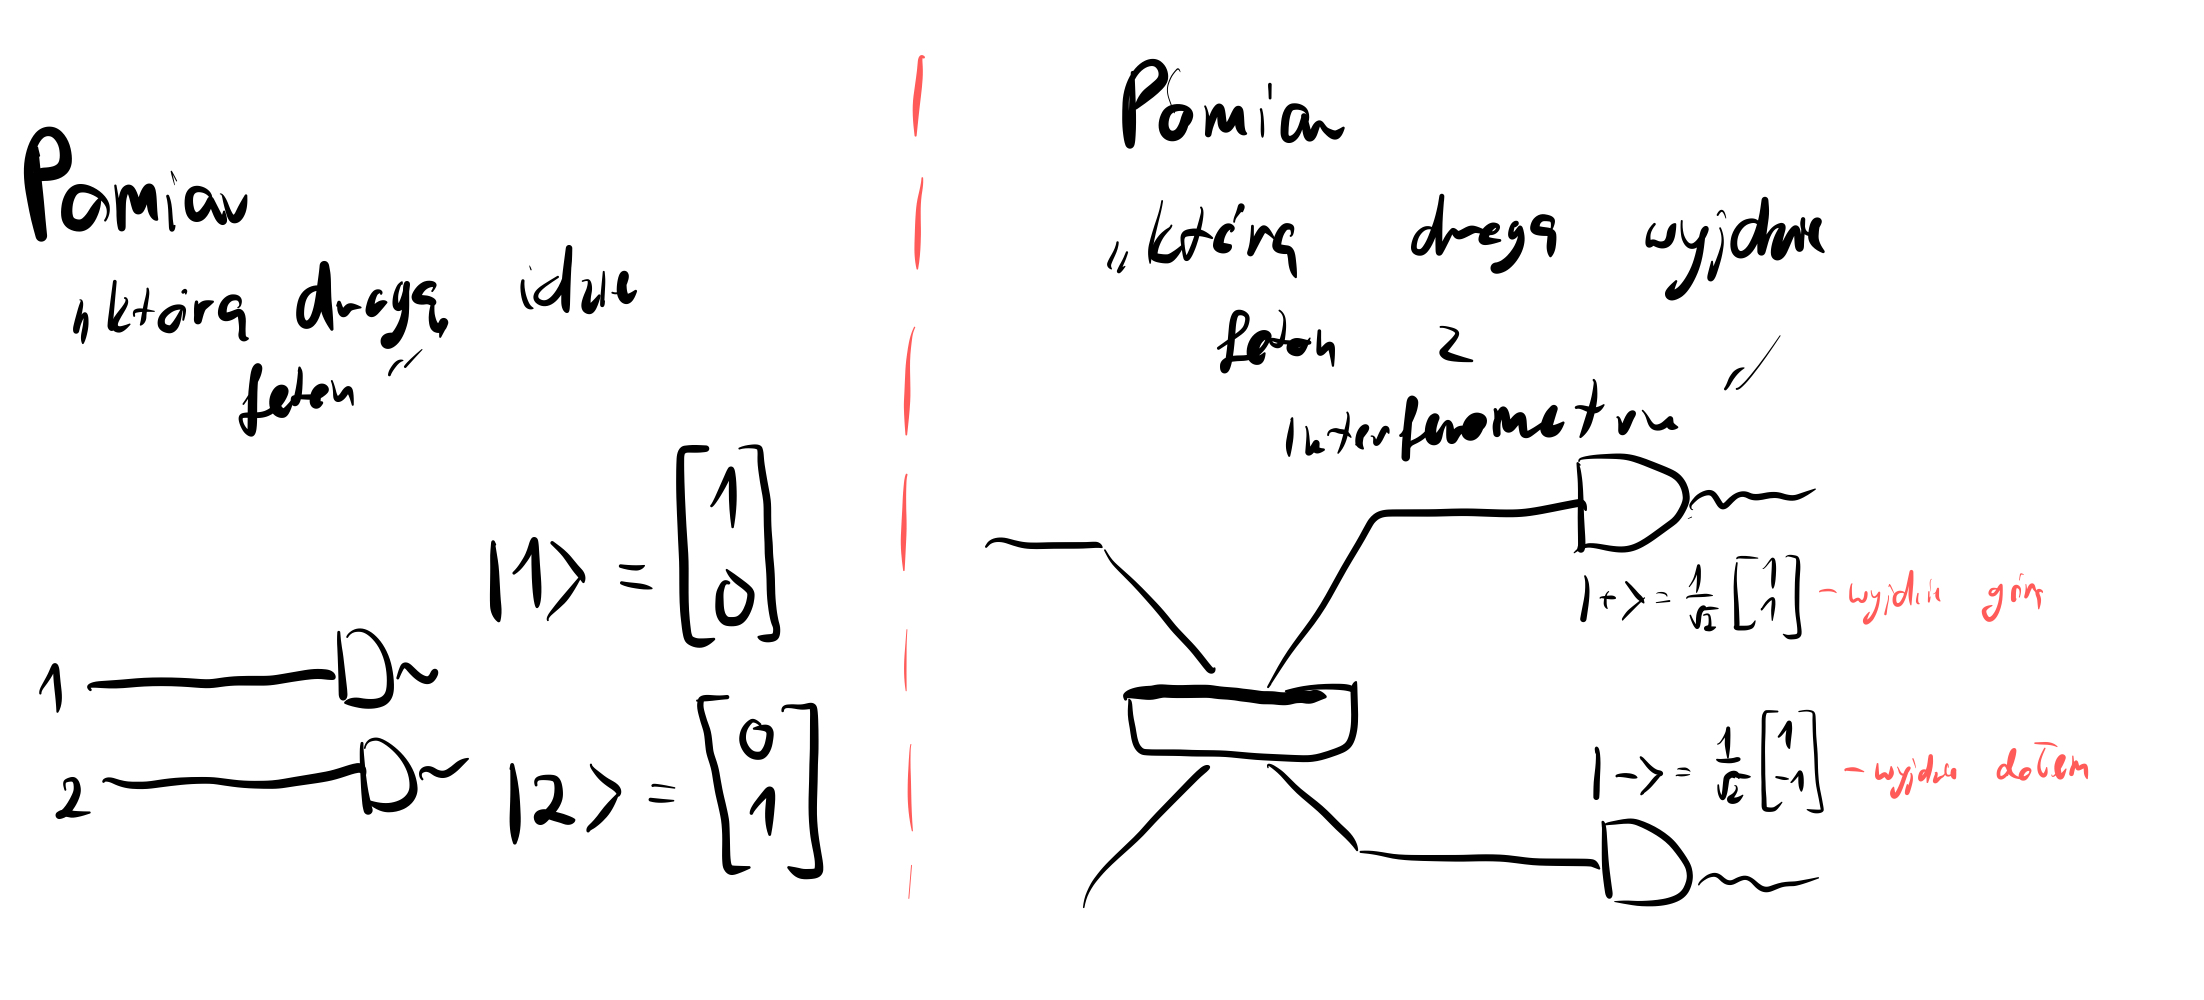
\includegraphics[width=0.8\linewidth]{Wyk_2_Rys_1.jpeg}
        \caption{Porównanie podejść myślenia o kwantu - deterministyczny i niedeterministyczny}
        \label{fig:lec_2:porownianie}
    \end{figure}
    

\begin{emph_box}{\ind{Postulat pomiarowy}}
    Jeśli $\ket{\Psi}$ jest dowolnym stanem, na którym chcemy zmierzyć wielkość fizyczną $A$, z którą stowarzyszona jest baza $\qty{\ket{a_i}}$. Możemy napisać:
    \[\ket{\Psi} = \sum_i \alpha_i\ket{a_i}\]
    Wtedy uzyskany wynik $a_i$ z prawdopodobieństwem $p_i = \qty|\alpha_i|^2 = \qty|\braket{a_i}{\Psi}|^2$. Tym samym stan po pomiarze ma dobrze określone wielkości $a_i$, tj. jest $\ket{\Psi} = \ket{a_i}$.
\end{emph_box}
 Czyli też jak już raz dokonamy pomiaru na stanie kwantowym to on już nie wróci do możliwości interferencji, i za każdym kolejnym pomiarem już będziemy obserwować ten sam stan, tj. zacznie się zachowywać jakby był klasyczny.
    
\ind{Obserwabla}:
Z pomiarem wielkości A $\qty(\qty{\ket{a_i}})$ stowarzyszamy operator 
\[
    \hat{A} = \sum_i a_i \ketbra{a_i}
\]
gdzie $\hat{A}$ jest operatorem Hermitowskim\footnote{Operator hermitowski - $A^\dagger = A$} czyli w szczególności mając $\hat{A}$ możemy też znaleźć $\qty{\ket{a_i}}$ robiąc rozkład własny.

\begin{align*}
\hline \hline
\end{align*}

{\it Crash course z notacji Diraca:}\\
\textbf{ket}:
\[
    \ket{a} = \mqty[a_1 \\ a_2 \\ \vdots \\ a_n] = \vb{v}
\]
\textbf{bra}:
\[
    \bra{a} = \ket{a}^\dagger = \mqty[a_1, a_2, \cdots, a_n]^\ast = \vb{v}^\dagger
\]
Czyli jak je połączymy dostajemy \textbf{braket}:
\[
    \braket{a}{b} = \mqty[a_1, a_2, \cdots, a_n]^\ast \cdot \mqty[b_1 \\ b_2 \\ \vdots \\ b_n] = \vb{v} \cdot \vb{v}^\ast = liczba\footnote{Iloczyn skalarny}
\]
Zaś z kolei jak pomnożymy w odwrotnej koleności mamy \textbf{ketbra}:
\[
    \ketbra{a}{b} =  \mqty[a_1 \\ a_2 \\ \vdots \\ a_n] \cdot \mqty[a_1, a_2, \cdots, a_n]^\ast = M \in M(\CS)_n^n
\] co rozumiemy też jako operator rzutowy.

\begin{align*}
\hline \hline
\end{align*}

Obserwable jest wygodniej liczyć jako wartości oczekiwane z jakichś rozkłądów prawdopodobieństw:\\
\[
    \expval{A} = \sum_i p_i a_i = \sum_i \qty|\braket{a_i}{\Psi}|^2 \cdot a_i
\]
Gdzie wiemy, że człon $\qty|\braket{a_i}{\Psi}|^2$ możemy rozpisać jako:
\[
    \qty|\braket{a_i}{\Psi}|^2 = \qty|\braket{\Psi}{a_i}|^2 = \braket{\Psi}{a_i}\braket{a_i}{\Psi} = \bra{\Psi} \quad \ketbra{a_i} \quad \ket{\Psi}
\]
W związku z tym możemy dalej rozpisać $\expval{A}$ jako:
\[
    \expval{A} = \bra{\Psi} \quad \sum_i a_i \ketbra{a_i} \quad \ket{\Psi} =\footnote{${\color{blue} \sum_i a_i \ketbra{a_i} = \hat{A}}$} \ev{\hat{A}}{\Psi}
\]

Further reading:
\begin{itemize}
    \item \link{http://studenci.fuw.edu.pl/~kc427902/Prezentacje_Kwanty/wyklad2-stanypomiary.pdf}{Notatki Demko do wykładu}
    \item \link{http://studenci.fuw.edu.pl/~kc427902/Prezentacje_Kwanty/cwiczenia2.pdf}{Zadania na ćwiczenia 2}
    \item \link{http://studenci.fuw.edu.pl/~kc427902/Prezentacje_Kwanty/cwiczenia2-sol.pdf}{Rozwiązania z ćwiczeń 2}
\end{itemize}
\end{lecture}

% --------------------------------------------------------
% Wykład 09.03.2022

\begin{lecture}{Ewolucja stanów kwantowych i Hamiltonian}
\section{Ewolucja stanów kwantowych}
Będziemy brać teraz pod uwagę tylko \emph{układy izolowane}! Tutaj rozumiemy, że \ind{Układ izolowany} - układ który nie oddziaływuje z otoczeniem i brak pomiarów.\\
Formalnie napiszemy, że (póki co bez żadnych założeń) $\ket{\Psi(0)}$ - stan w chwili początkowej, $\ket{\Psi(t)}$ - stan po czasie. Teraz chcemy wiedzieć, jaki będzie $\ket{\Psi(t)}$?
Otóż:
\[
    \ket{\Psi(0)} = \mathcal(U)(t)\qty[\ket{\Psi(0)}]
\]
Tj. tak jak w mechanice klasycznej - założymy, że nasza ewolucja w czasie jest odwracalna. Wynika z tego, że 
\begin{itemize}
    \item \emph{stany rozróżnialne\footnote{Ortogonalne} muszą pozostać rozróżnialne.} Możemy na to patrzeć jako na \emph{zachowanie informacji}.
    \[
        \braket{\Psi(0)} = 0 \qc \braket{\Psi(t)} = 0
    \]
    \item Stopień rozróżnialności tych stanów zależeć będzie od ich iloczynu skalarnego. Chcemy, żeby pozostał on stały $$\implies \braket{\Psi(0)} = \braket{\Psi(t)}$$
\end{itemize}

{\color{teal} Fakt}: $U(t)$ jest liniowe.\\
Sprawdźmy go. Także rozważmy $$\ket{\xi} = U(t)\qty[a \ket{\Psi(0)} + b \ket{\Psi(0)}] - a U(t)\qty[\ket{\Psi(0)}] - b U(t)\qty[\ket{\Psi(0)}]$$
Teraz obliczmy:
\begin{align*}
    \braket{\xi} &= \qty(U(t) \qty[a \psket{0} + b \psket{0}])^\dagger \qty( U(t) \qty[a \ket{\Psi(0)} + b \ket{\Psi(0)}] - a U(t) \qty[\ket{\Psi(0)}] - b U(t) \qty[\ket{\Psi(0)}])\\
    &- \qty(a U(t) \qty[\psket{0}])^\dagger \qty(-||-)\\
    &- \qty(a U(t) \qty[\psket{0}])^\dagger \qty(-||-)
\end{align*}
Czyli $\qty(U(t)\ket{\Psi})^\dagger (U(t) \ket{\Psi}) = \braket{\Psi} = 0$, bo można 'usunąć' wszystkie $U(t)$. Wynika z tego, że $U(t)$ \emph{jest liniowe.}

{\color{teal} Wnioski}: $U(t)$ jest liniowa (w skończenie wymiarowych przestrzeniach reprezentowanych przez macierz\footnote{Bo $(AB)^\dagger = A^\dagger B^\dagger$}) i zachowuje iloczyn skalarny.
\[
    \implies \psket{0} = U(t) \cdot \psket{0}
\]

Teraz ciągnąc to rozumowanie dalej:
\[
    \forall_{\ket{\Psi(0)}, \ket{\varphi(0)}} = \braket{\Psi(0)}{\varphi(0)} = \mel{\Psi(0)}{U^\dagger(t) U(t)}{\varphi(0)} = \braket{\Psi(0)}{\varphi(0)}
\]
Wynikać z tego będzie, że $U(t)^\dagger U(t) = 1$. Wiedząc, że pracujemy w skończenie wymiarowej przestrzeni wnioskujemy, że $U(t)$ jest \emph{Unitarne}. Oznacza to też, że $U^{-1}(t) = U(t)^\dagger$. Teraz fizycznym argumentem, że $U^{-1}(t)$ istnieje będzie to, że powinno być $U^{-1}(t) = U(-t)$.\\

Idziemy dalej. Wiemy, że $U(t=0) = \Id$. Rozważmy pierwsze (liniowe) rozwinięcie $U(t)$ w czasie:
\[
    U(dt) = \Id + \qty(- \frac{i}{\hbar} H \dd{t} + O(\dd{t}^2))
\]
\[
1 = U(\dd{t})^\dagger U(\dd{t}) = \qty(\Id + \frac{i}{\hbar} H^\dagger \dd{t} + O(\dd{t}^2)) \qty(\Id - \frac{i}{\hbar} H^\dagger \dd{t} + O(\dd{t}^2)) = \Id + \frac{i}{\hbar} (H^\dagger - H) \dd{t} + O(\dd{t}^2)
\]
Czyli widzimy, że $H^\dagger = H$ - jest Hermitowskie.

\[
    \psket{\dd{t}} = U(\dd{t}) \psket{0} = \psket{0} - \frac{i}{\hbar} H \dd{t} \psket{0} + O(\dd{t^2}) = \psket{0} + \dv{\psket{t}}{t}\eval_{t=0} + \order{\dd{t^2}}
\]
\[
    \dv{\psket{t}}{t}\eval_{t=0} = - \frac{i}{\hbar} H \psket{0} \implies i \hbar \dv{\psket{t}}{t}\eval_{t=0} = H \psket{0}
\]Ale zamiast pisać $\psket{\dd{t}} = U(\dd{t}) \psket{0}$ można ogólniej powiedzieć: $\psket{t + \dd{t}} = U(\dd{t}) \psket{t}$.\\
Dostajemy krypto \subind{Równanie Schrödingera}{Równanie!Schrödingera}:
\begin{equation}
    i \hbar \dv{\psket{t}}{t} = H \psket{t}
    \label{eq:lec_3:krypto_schrodinger}
\end{equation}
(Krypto, bo nie znamy natury $H$)

\section{Argument za naturą fizyczną H}
Rozważmy obserwablę $A$ i jej wartość oczekiwaną na stanie $\psket{t}$.
Wtedy:
\[
    \ev{A}_t = \ev{A}{\Psi(t)}
\]
\begin{align*}
    \dv{\ev{A}_t}{t} &= \dv{\bra{\Psi(t)}}{t} A \psket{t} + \ev{A}{\Psi(t)} = \frac{i}{\hbar} \ev{H\cdot A - A \cdot H}{\Psi(t)}\\
    &= \frac{i}{\hbar} \ev{\qty[H, A]}{\Psi(t)} = - \frac{i}{\hbar} \ev{\qty[A, H]}{\Psi(t)}
\end{align*}

Jeśli wybierzemy $A = H \implies \dv{\ev{H}}{t} = 0$ czyli H jest związany z wielkością fizyczną zachowaną w czasie ewolucji $\implies$ w
pierwsza myśl, że ma coś wspólnego z energią.

\begin{emph_box}{Analogia z Mechaniką Klasyczną}
$$A(q, p) \qc \dv{A}{t} = \qty{A, H} = \sum_i \dv{A}{q_i} \dv{H}{p_i} - \dv{A}{p_i}\dv{H}{q_i}$$
Formalna recepta wiążąca mechanikę klasyczną z kwantową: $$\qty{\cdot, \cdot} \to =-\frac{i}{\hbar} \qty[\cdot , \cdot]$$
Jest to dodatkowy argument na to, że H ma coś wspólnego z energią.
\end{emph_box}

To teraz dochodzimy do równań:
\[
    \dv{\psket{t}}{t} = - \frac{i}{\hbar} H \psket{t} \implies \psket{t} = U(t) \psket(0)
\]
Gdzie $U(t) = e^{- \frac{i}{\hbar}H \cdot  t}$
Gdzie wreszcie piszemy, że H - Hamiltonian.

\section{Wyznaczenie ewolucji stanu w praktyce}

Mamy $H$, robimy jego rozkład własny, tj. $H = \sum_k E_k\footnote{Wartości własne (energie)}\ketbra{E_k}$. $H\ket{E_k} = E_k\ket{E_k}$

Jeśli:\\
$\psket{0} = \ket{E_k}, \qq{stan o dobrze określonej energii}$\\
$\psket{t} = e^{- \frac{i}{\hbar}H \cdot  t} \ket{E_k} = e^{- \frac{i}{\hbar}E_k \cdot  t} \ket{E_k}$\\
Czyli energia stanu o dobrze określonej energii zmienia tylko globalną fazę, czyli fizycznie stan się nie zmienia.\\
Ogólnie jeśli mamy dowolny stan początkowy $\psket{0}$, to możemy go rozłożyć w bazie $\qty{\ket{E_k}}$. W takim razie widzimy, że zajdzie:\\
$\psket{0} = \sum_k c_k\footnote{$c_k = \braket{E_k}{\Psi(0)}$} \ket{E_k}$, z liniowości $\psket{t} = \sum_k c_k U(t)\ket{E_k} = \sum_k c_k e^{- \frac{i}{\hbar}E_k \cdot t} \ket{E_k}$\\
\emph{Uogólnienie} W modelach gdy $H$ zależy jawnie od czasu (czyli de facto bierzemy układ izolowany) możemy te układy wciąż opisywać jakby były izolowane, ale musimy dopuścić $H = H(t)$. Wtedy jedyna zmiana jaka się pojawia, to:
\[
    \dv{\psket{t}}{t} = - \frac{i}{\hbar} H(t) \psket(t) \implies U(t) \approx e^{- \frac{i}{\hbar} (t - \Delta t) \Delta t} \dots e^{- \frac{i}{\hbar} (\Delta t) \Delta t} e^{- \frac{i}{\hbar} (0) \Delta t}
\]
\[
    U(t) \approx
    \begin{cases}
        U(t) = e^{- \frac{i}{\hbar} \int_0^t H(t) \dd{t}}, \qq{jeśli H(t) komutują ze sobą w różnych chwilach czasu}\\
        U(t) = \tau\footnote{uporządkowanie czasowe} \qty[e^{- \frac{i}{\hbar} \int_0^t H(t) \dd{t}},]
    \end{cases}
\]
\end{lecture}

% --------------------------------------
% 11.03.22

\renewcommand{\psket}[1]{\ket{\Psi(#1)}}

\begin{lecture}{Równanie Schrodingera (na koszulkach)}
\section{Schizofreniczna Ewolucja}

\begin{figure}[!ht]
        \centering
        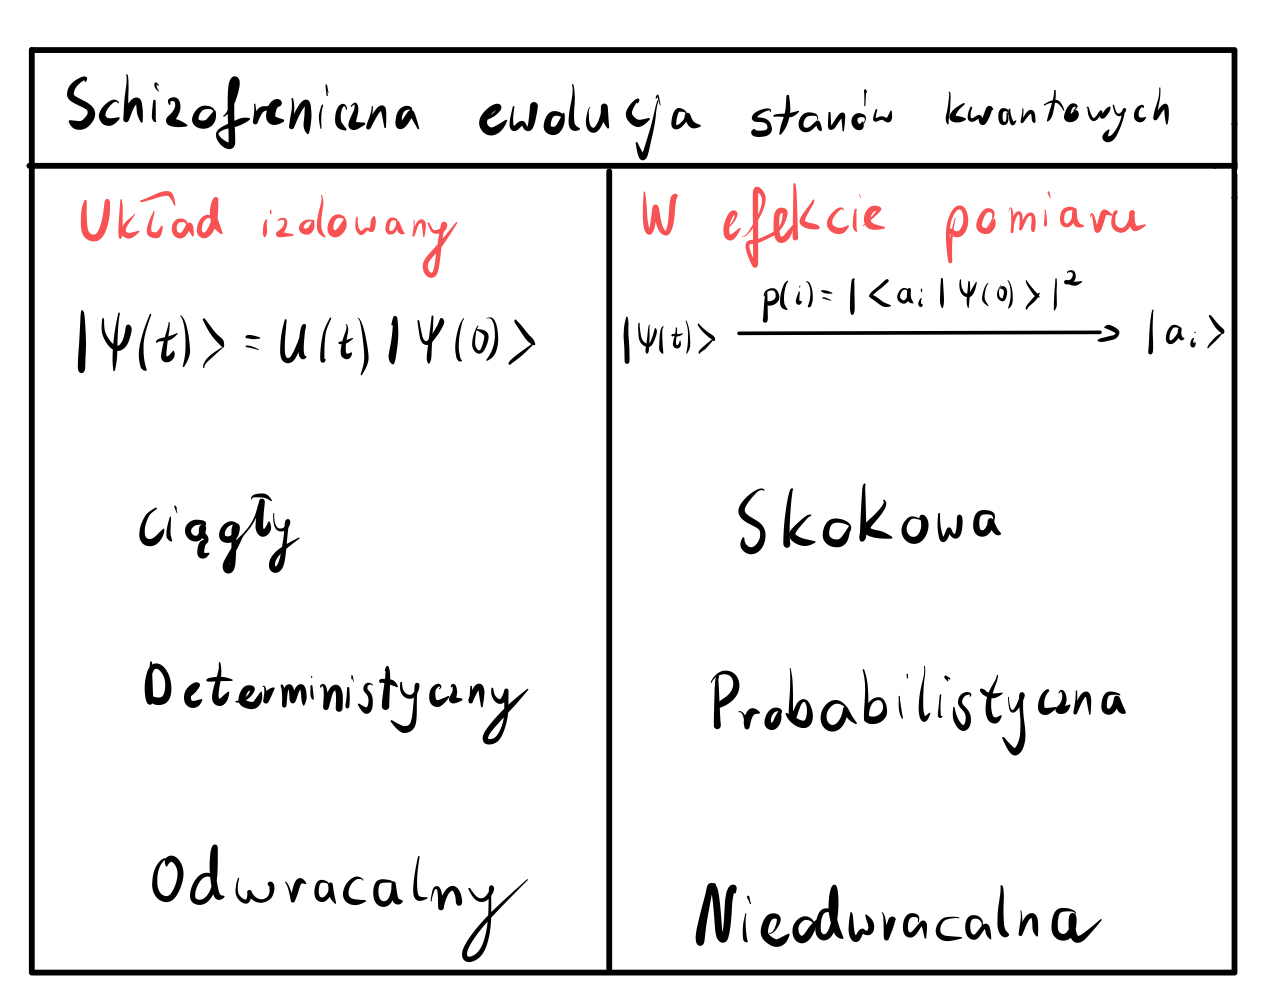
\includegraphics[width=\linewidth]{Wyk_4_Rys_1.jpeg}
        \caption{Schizofreniczna Ewolucja}
        \label{fig:lec_4:tabelka}
\end{figure}

\section{Kwantowy Efekt Zenona (z Elei)}
Formułował wiele paradoksów - miał dobrą intuicję. Jeden z bardziej znanych - \emph{paradoks strzały}\\
\textit{Paradoks strzały} - Skoro strzała w każdej chwili spoczywa, to ruch jest niemożliwy.

Rozważmy układ kwantowy, którego ewolucja jest opisana Hamiltonianem $\HS$.
\begin{itemize}
    \item Stan początkowy $\psket{0}$ nie będzie stanem własnym $\HS$ (żeby ewoluował nietrywialnie).
    \item Wtedy ewolucja po czasie $t$: $\psket{t} = e^{- \frac{i\HS t}{\hbar}}\psket{0}$ i sprawdzamy, czy układ wciąż jest w stanie $\psket{0}$ \footnote{Czyli wykonujemy pomiar w bazie ortonormalnej, której jednym z wektorów jest $\psket{0}$}
    \item Prawdopodobieństwo, że stan pozostał niezmieniony: \\$p(t) = \qty|\braket{\Psi(0)}{\Psi(t)}|^2 = \braket{\Psi(0)}{\Psi(t)}\braket{\Psi(t)}{\Psi(0)} = \ev{e^{- \frac{i\HS t}{\hbar}}}{\Psi(0)} = \ev{e^{\frac{i\HS t}{\hbar}}}{\Psi(0)}$\\
    Wtedy po rozwinięciu dla małych $t$ \footnote{$e^x \approx 1 + x + \frac{x^2}{2} + \order{x^3}$}:
    \begin{align*}
        p(t) &= 1 + t \cdot \qty[\ev{- \frac{i\HS}{\hbar}}{\Psi(0)} \braket{\Psi(0)} + \braket{\Psi(0)} \ev{\frac{i\HS}{\hbar}}{\Psi(0)} ] + \\
        &- t^2\cdot \qty[\ev{\frac{\HS^2}{\hbar^2}}{\Psi(0)} \braket{\Psi(0)} + \frac{1}{2} \braket{\Psi(0)} \ev{\frac{\HS^2}{\hbar^2}}{\Psi(0)} - \ev{\frac{\HS}{\hbar}}{\Psi(0)}\ev{\frac{\HS}{\hbar}}{\Psi(0)}] + \order{t^3} \\
        &= 1 + \frac{t^2}{\hbar^2} \underbrace{(\ev{\HS^2}{\Psi(0)} - \ev{\HS}{\Psi(0)}^2)}_{\Delta^2 \HS\footnotemark} + \order{t^3}
    \end{align*}
    \footnotetext{Stan ewoluuje 'tym szybciej' im ma większą ma wariancję $\HS$}
    Czyli wyobrażamy sobie, że mierzymy stan coraz częściej, czyli n razy co czas $\frac{t}{n}$, pytamy jakie jest prawdopodobieństwo , że we wszystkich $n$ pomiarach okaże się, że stan pozostaje $\psket{0}$
    \item Czyli finalnie to prawdopodobieństwo, to:
    $p_n = \qty(\qty|\braket{\Psi(0)}{\Psi(t)}|^2)^n = \qty[1 - \frac{\Delta^2\HS}{\hbar^2} (\frac{t}{n})^2 + \order{t^3}]^n$\\
    $p_n \stackrel{n\to\infty}{\approx} 1 - \frac{\Delta^2\HS t^2}{\hbar^2} \cdot \frac{1}{n} \order{\frac{1}{n^2}} \stackrel{n\to\infty}{\approx} 1$
    \item Rozumiemy to tak, że bardzo częsty pomiar 'zamraża' ewolucję stanu.
\end{itemize}
    
\section{Równanie Schrodingera (na koszulkach)}

Nierelatywistyczna, punktowa cząstka kwantowa mogąca się poruszać w przestzeni. Dla uproszczenia myślimy na razie o 1D.\\
Jeśli przestrzeń byłaby fundamentalnie zdyskretyzowana, tj. $x_i\footnote{\text{Dopuszczalne położenia}} \in \qty{\dots, -2\Delta, -\Delta, 0,  \Delta, 2 \Delta, \dots}$, $\ket{x_i}$ - stany położeniowe (rozróżnialne) reprezentujące, że cząstka znajduje się w punkcie $x_i$.\\
Ogólny stan: $\ket{\Psi} = \sum_i \Psi_i \ket{x_i} \qc \sum_i \qty|\Psi_i|^2 = 1 \qc \braket{x_i}{x_j} = \delta_{ij}$\\
Wygodnie jest rozważyć granicę \emph{ciągłą}:
\[
    \ket{\Psi} = \int \dd{x} \Psi(x) \ket{x}
\]
Gdzie $\qty|\Psi(x)|^2$ - gęstość prawdopodobieństwa znalezienia cząstki w punkcie $x$. \\
Skoro chcemy, żeby $\braket{\Psi} = 1^{(i)} \implies \int \dd{x} \qty|\Psi(x)|^2 = 1^{(ii)}$. Czyli:\\
$\braket{\Psi} = \int \dd{x} \Psi^\ast(x) \bra{x} \int \dd{x} \Psi(x') \ket{x'} \implies \int \dd{x} \dd{x'} \Psi^\ast(x) \Psi(x) \braket{x}{x'} \stackrel{(i), (ii)}{\implies} \braket{x}{x'} = \delta(x-x')\footnote{Czyli o $\ket{x}$ można myśleć jako o pewnej bazie ortogonalnej, ale nie unormowanej, bo $\braket{x} = \infty$}$.
\subind{Funkcja falowa}{Funkcja!falowa} - funkcja gęstości prawdopodobieństwa $\Psi(x)$ o amplitudzie $\qty|\Psi(x)|^2$. Jest ona reprezentacją położeniową stanu $\ket{\Psi}$\\
Zauważmy: $\ket{Psi} = \int \dd{x} \Psi \ket{x}$, $\ket{\varphi} = \int \dd{x'} \varphi(x') \ket{x'}$
\[
    \braket{\Psi}{\varphi} = \int \dd{x} \dd{x'} \Psi^\ast(x) \varphi(x') \underbrace{\braket{x}{x'}}_{\delta(x-x')} = \int \dd{x} \Psi^\ast(x) \varphi(x)
\]
Możemy teraz zdefiniować operator (\subind{Obserwabla Położenia}{Obserwabla!Położenia}):
\[
    \hat{x} = \int \dd{x} x \ketbra{x} \qc \hat{x} \ket{x} - \int \dd{x'} x' \ketbra{x'} \ket{x} = x \ket{x}
\]
Teraz zauważmy, że warunkiem zupełności bazy będą:
{\color{orange} (Fakt)} $\underbrace{\int \dd{x} \ketbra{x}}_C = \Id$\\

{\color{orange} (Dowód)} Weźmy dwa dowolne $\ket{x'}, \ket{x''}$
\[
    \mel{x'}{C}{x''} = \int \dd{x} \braket{x'}{x} \underbrace{\braket{x}{x''}}_{\delta(x-x'')} = \braket{x'}{x''} = \mel{x'}{\Id}{x''} \implies C= 1 \quad \Box
\]
Czyli:
\[
    \ket{\Psi} = \int \dd{x'} \Psi{x'} \ket{x'} \implies \Psi(x) = \braket{x}{\Psi}
\]
Pamiętamy, że $ i \hbar \dv{\psket{t}}{t} = \HS \psket{t}$. Teraz żeby napisać $\HS$ kwantowo potrzebujemy $\hat{p}$
\[
    \HS = \frac{p^2}{2m} + V(x) \qq{kwantowo} \to \hat{\HS} = \frac{\hat{p}^2}{2m} + V(\hat{x})
\]

\emph{Operator Pędu}:\\
Intuicja falowa (świetlna), fale płaskie (stany o dobrze określonej energii i pędzie)
\[
    \Psi(x, t) \sim e^{i (kx - \omega t)}
\]
Hipoteza Plancka/ De Broigle'a $E = \hbar \omega$,  $p = \frac{h}{\lambda} = \hbar \cdot k$\\
żeby $\hat{p} \Psi(x, t) = p \Psi(x, t) = \hbar k \Psi(x, t)$ trzeba wziąć $\hat{p} = \frac{\hbar}{i}$\\

Further reading:
\begin{itemize}
    \item \link{http://studenci.fuw.edu.pl/~kc427902/Prezentacje_Kwanty/wyklad3-ewolucja.pdf}{Notatki Demko do wykładu}
    \item \link{http://studenci.fuw.edu.pl/~kc427902/Prezentacje_Kwanty/cwiczenia3.pdf}{Zadania na ćwiczenia 3}
    \item \link{http://studenci.fuw.edu.pl/~kc427902/Prezentacje_Kwanty/cwiczenia3-sol.pdf}{Rozwiązania z ćwiczeń 3}
\end{itemize}

\end{lecture}

% ------------------------------------------------------------------
% Wykład 16.03.2022


\begin{lecture}{Równanie Schrödingera, propagator i całki po trajektoriach et al.}

\section{Powtórka z poprzedniego wykładu}

\subsection{Reprezentacja położeniowa a pędowa}

W reprezentacji położeniowej:\\
\[
    \hat{x} \ket{x} = x \ket{x} \qc \hat{x} \ket{\Psi} = \hat{x} \int \dd{x} \Psi(x) \ket{x} = \int \dd{x} \Psi(x) \hat{x} \ket{x} = \int \dd{x} \underbrace{\Psi(x) x}_{\footnotemark} \ket{x}
\]
\footnotetext{Efektywne działanie $\hat{x}$ w reprezentacji położeniowej}
Czyli widzimy, że zachodzi $\ket{\Psi} \stackrel{\hat{x}}{\to} \hat{x} \ket{\Psi} \equiv \Psi(x) \to x \cdot \ket{\Psi}$\\
Zachodzi również:
\begin{itemize}
    \item $\qty{ \cdot, \cdot} \to - \frac{i}{\hbar} \qty[\cdot , \cdot]$
    \item $\qty[\hat{x}, \hat{p}] = i \hbar \cdot \Id$
    \item $\qty[\hat{x}, \hat{p}] \ket{\Psi} = i \hbar \ket{\Psi}$ w reprezentacji położeniowej.
    \item $(x \cdot \hat{p} - \hat{p} \cdot x) \Psi(x) = i \hbar \Psi(x)$\\
    $x \underbrace{\hat{p}[\Psi(x)]}_{\footnotemark} - \hat{p} \qty[x \cdot \Psi(x)] = i \hbar \Psi(x)$
\end{itemize}
\footnotetext{Działanie $\hat{p}$ w reprezentacji położeniowej}

\section{Równanie Schrödingera}

\begin{emph_box}{\subind{Równanie Schrödingera}{Równanie!Schrödingera}}
\begin{equation}
    i \hbar \pdv{\Psi(x, t)}{t} = - \frac{\hbar^2}{2m} \pdv[2]{x} \Psi(x) + V(x) \Psi(x, t)
    \label{eq:lec_5:schrodinger}
\end{equation}
\end{emph_box}

Wiemy, że ogólnie ewolucję liczymy:
\begin{align*}
    \psket{t} = \sum_k \braket{E_k}{\Psi(0)} e^{- \frac{i E_k t}{\hbar}} \ket{E_k}\\
    \braket{x}{\Psi(x)} = \sum_k e^{- \frac{i E_k t}{\hbar}} \braket{E_k}{\Psi(0)}  \braket{x}{E_k}\\
    \Psi(x) = \sum_k \braket{E_k}{\Psi(0)} e^{- \frac{i E_k t}{\hbar}}  \underbrace{\phi_{E_k}(x)}_{\footnotemark}
\end{align*}
\footnotetext{Funkcja falowa stanu własnego $\hat{\HS}$ (stan stacjonarny)}
Czyli wystarczy zmienić $\phi_{E_k}(x)$ i $E_k$, żeby znaleźć ewolucję $\hat{\HS} \qty[\phi_{E_k}(x)] = E_k \phi_{E_k}(x)$ co daje nam:
\begin{emph_box}{\subind{Równanie Schrödingera bez czasu}{Równanie!Schrödingera!bez czasu}}
\begin{equation}
    \qty[- \frac{\hbar^2}{2m} \dv[2]{x} + V(x)] \phi_{E_k}(x) = E_k \phi_{E_k} (x)
    \label{eq:lec_5:schrodinger_nzal_czas}
\end{equation}
    Znane skrótowo jako:
    \begin{equation}
        \hat{H} \ket{\Psi} = E \ket{\Psi}
        \label{eq:lec_5:schrodinger_bez_czasu}
    \end{equation}
    Ta niezależna od czasu reprezentacja równania schrödingera de facto jest problemem szukania stanów własnych Hamiltonianu. Czyli rozwiązując ewolucję Hamiltonianu w czasie najpierw rozwiązujemy problem znajdywania stanów, a dopiero potem szukamy jego ewolucji czasowej, tj zgodnie z równaniem \eqref{eq:lec_5:schrodinger}.
\end{emph_box}
\subsection{Cząstka swobodna}
Gdzie dla cząstki swobodnej wygląda to tak, że $V(x) = 0$:
\begin{align*}
    - \frac{\hbar^2}{2m} \dv[2]{x} \Psi(x) &= E \Psi(x)\\
    \dv[2]{x} \Psi(x) &= - \frac{2m E}{\hbar^2} \Psi(x)\\
    \text{Gdzie rozwiązania to kombinacje liniowe  } &e^{\pm i \frac{2 m E}{\hbar^2}} \text{tj. Fale płaskie będące jednocześnie stanami własnymi }\hat{p}\\
    \implies \hat{p} e^{i px/\hbar} &= \frac{\hbar}{i} \dv{x} e^{i p x/ \hbar} = p \cdot e^{i p x / \hbar}\\
    \text{Czyli będziemy rozkładać na } &\text{stany własne w reprezentacji pędowej:}\\
    \Psi_p(x) = \frac{1}{\sqrt{2 \pi \hbar}} e^{i p x /\hbar} &\qc p = \pm \sqrt{2 m E}\\
    \text{Wtedy widzimy, że }&\text{ewolucja prosta:}\\
    \Psi_p(x, t) &= \Psi_p(x) e^{- \frac{i E t}{\hbar}} = \Psi_p(x) e^{- \frac{i p^2 t}{2 m \hbar}} \\
    \text{Czyli ewolucja }&\text{ogólnego stanu:}\\
    \Psi(x,t) &= \frac{1}{\sqrt{2 \pi \hbar}} \int \dd{p} \underbrace{\braket{p}{\Psi(0)}}_{\footnotemark} \cdot e^{- \frac{i p x}{\hbar} - \frac{i p^2 t}{2 m \hbar}}
\end{align*}
\footnotetext{Rozkład na stany własne pędu$ = \tilde{\Psi}(p, 0)$ - reprezentacja pędowa}

\section{Historia rozwoju Mechaniki Kwantowej}
Były dwie szkoły \sout{Falenicka i Otwocka} Heisenberga i Schrödingera:
\begin{itemize}
    \item Schrödinger - Mechanika falowa opis poprzez funkcje falowe.
    \item Heisenberg - Mechanika Macierzowa, opis poprzez obserwable
\end{itemize}
\section{Obraz Schrödingera i obraz Heisenberga}
\label{sec:lec_5:schrodinger_heisenberg}
\emph{Obraz Schrödingera}:\\
$\ket{\Psi} = U(t) \psket{0}\qc U(t) = e^{- \frac{i \HS t}{\hbar}}$. Jeśli liczymy wartość oczekiwaną obserwabli w czasie $t$: $\ev{A}_t = \ev{\hat{A}}{\Psi(t)} = \ev{U^\dagger(t) \hat{A} U(t)}{\Psi(0)}$\\
Możemy jednak spojrzeć na to jak na sytuację, gdzie stan układu nam się nie zmienia, a zmieniają się obserwable. Daje nam to:\\
\emph{Obraz Heisenberga}:\\
$\ket{\Psi^{(H)}(t)} = \psket{0} \qc \hat{A}^{(H)} := U^\dagger (t) \hat{A} U(t)\qc \ev{A}_t = \ev{A^{(H)}(t)}{\Psi(0)}$\\
Ewolucja obserwabli jest opisana przez równanie Heisenberga:\\
\[
    \dv{t} \hat{A}^{(H)}(t) = \qty(\dv{t} U^\dagger (t)) \hat{A} U(t) + U^\dagger(t) \hat(A) \dv{t} U(t) = \frac{i}{\hbar} \qty[U^\dagger(t) \hat{\HS} \hat{A} U(t) - U^\dagger \hat{A} \hat{\HS} U(t)] = \frac{i}{\hbar} \qty[\hat{\HS}\hat{A}^{(H)} - \hat{A}^{(H)}\hat{\HS}]
\]
Czyli finalnie dostajemy:

\begin{emph_box}{\subind{Równanie Heisenberga}{Równanie!Heisenberga}}
    \begin{equation}
        \dv{\hat{A}^{(H)}(t)}{t} = \frac{i}{\hbar} \qty[\hat{\HS}, \hat{A}^{(H)}(t)]
        \label{eq:lec_5:heisenberg}
    \end{equation}
\end{emph_box}

Further reading:
\begin{itemize}
    \item \link{http://studenci.fuw.edu.pl/~kc427902/Prezentacje_Kwanty/wyklad4-schroedinger.pdf}{Notatki Demko do wykładu}
    \item \link{http://studenci.fuw.edu.pl/~kc427902/Prezentacje_Kwanty/cwiczenia4.pdf}{Zadania na ćwiczenia 4}
    \item Tu będą Rozwiązania z ćwiczeń 4
\end{itemize}

\section{Propagator i całki po trajektoriach}
Ewolucja w reprezentacji położeniowej:
\[
    \overbrace{\braket{x}{\Psi(t)}}^{\Psi(x,t)} = \sum_k e^{- \frac{i E_k (t- t_0)}{\hbar}} \bra{E_k} \underbrace{\Id}_{\int \dd{x_0} \ketbra{x_0}} \ket{\Psi(t_0)} \braket{x}{E_k} = \int \dd{x_0} \sum_k e^{- \frac{i E_k (t- t_0)}{\hbar}} \underbrace{\braket{E_k}{x_o}}_{\phi^\ast_k(x_0)} \overbrace{\braket{x_0}{\Psi(t_0)}}^{\Psi(x_0, t_0)} \underbrace{\braket{x}{E_k}}_{\phi_k(x)}
\]
\[
    \Psi(x, t) = \int \dd{x_0} \qty(\sum_k \phi_k(x) \phi_k^\ast(x_0) e^{- \frac{i E_k (t-t_0)}{\hbar}}) \Psi(x_0, t_0)
\]
\begin{emph_box}{\subind{Propagator}{Funkcja!Greena} \index{Propagator}}
Możemy powiedzieć, że $K(x, t, x_0, t_0)$ to \emph{Propagator}
\begin{equation}
    K(x, t, x_0, t_0) = \SumInt_k \phi_k(x) \phi_k^\ast(x_0) e^{- \frac{i E_k (t-t_0)}{\hbar}}
    \label{eq:lec_5:propagator}
\end{equation}
Jak można łatwo zauważyć, propagator kwacze jak kaczka, chodzi jak kaczka, wygląda jak kaczka, więc jest to szukana \emph{Funkcja Greena}\footnotemark.\\

Ważna własność propagatora:
\[
    K(x, t_0, x_0, t_0) = \SumInt_k \phi_k(x) \phi_k^\ast(x_0)\footnotemark = \delta(x-x_0)
\]
\end{emph_box}
\addtocounter{footnote}{-1}
\footnotetext{Oh no... PTSD activated}
\refstepcounter{footnote}
\footnotetext{Pamiętamy, że $\sum_k \phi_k(x) \phi^\ast_k(x) = \sum_k \braket{x}{E_k}\braket{E_k}{x} = \mel{x}{\delta(x-x_0)}{x_0}$}
\emph{Przykład}: Propagator cząstki swobodnej\\
\[
    K(x, t, x_0, t_0) = \frac{1}{2 \pi \hbar} \int \dd{p} e^{\frac{i p x}{\hbar} - \frac{i (t - t_0)}{2 m \hbar}p^2}
\]
Co mając w głowie \emph{bardzo przyjemną własność matematyczną}:
\[
    \int_{-\infty}^{\infty} \dd{x} e^{-ax^2 + bx} = \sqrt{\frac{\pi}{a}} e^{\frac{b^2}{4 a}} \qq{co działa nawet dla liczb zespolonych, gdy }\Re(a)\geq0
\]
Dostajemy:
\[
    K(x, t, x_0, t_0) \stackrel{\Re(a) = 0\footnotemark}{=} \sqrt{\frac{m}{2 \pi \hbar \qty|y - y_0|}} e^{\frac{i}{\hbar} \frac{m (x - x_0)^2}{2 \qty|t-t_0|}}
\]
\footnotetext{W sensie dystrybucyjnym}

\end{lecture}

% ----------------------------------------------------------------------
% Wykład 18.03.2022

\begin{lecture}{Propagator et al.}

\section{Ad Propagator}
Kolejna ciekawa obserwacja:
\[
    U\footnotemark(t - t_0) = U(t- t_1) U(t_1-t_0)
\]
\footnotetext{$U(t)$ jak w Sekcji \ref{sec:lec_5:schrodinger_heisenberg}}
Teraz zapisując to na propagatorach dostajemy:
\[
    \Psi(x, t) = \int \dd{x_0} \dd{x_1} K(x, t, x_0, t_0) K(x_1, t_1, x_0, t_0) \Psi(x,t)
\]
To teraz możemy zagęścić atmosferę ($t_k$):
\[
    \Psi(x, t) = \int \dd{x_0} \dd{x_1} \dd{x_2} \dots K(x, t, x_n, t_n) K(x_n, t_n, x_{n-1}, t_{n-1}) \dots K(x_1, t_1, x_0, t_0)
\]

Teraz przechodzimy do granicy z $n\to\infty$ mamy de facto "sumowanie" po wszystkich drogach jakimi porusza się cząstka, trochę jak Zasada Huygensa dla optyki. Twochę jak przechodzenie z reprezentacji położeniowej na pędową.

\begin{figure}[!ht]
        \centering
        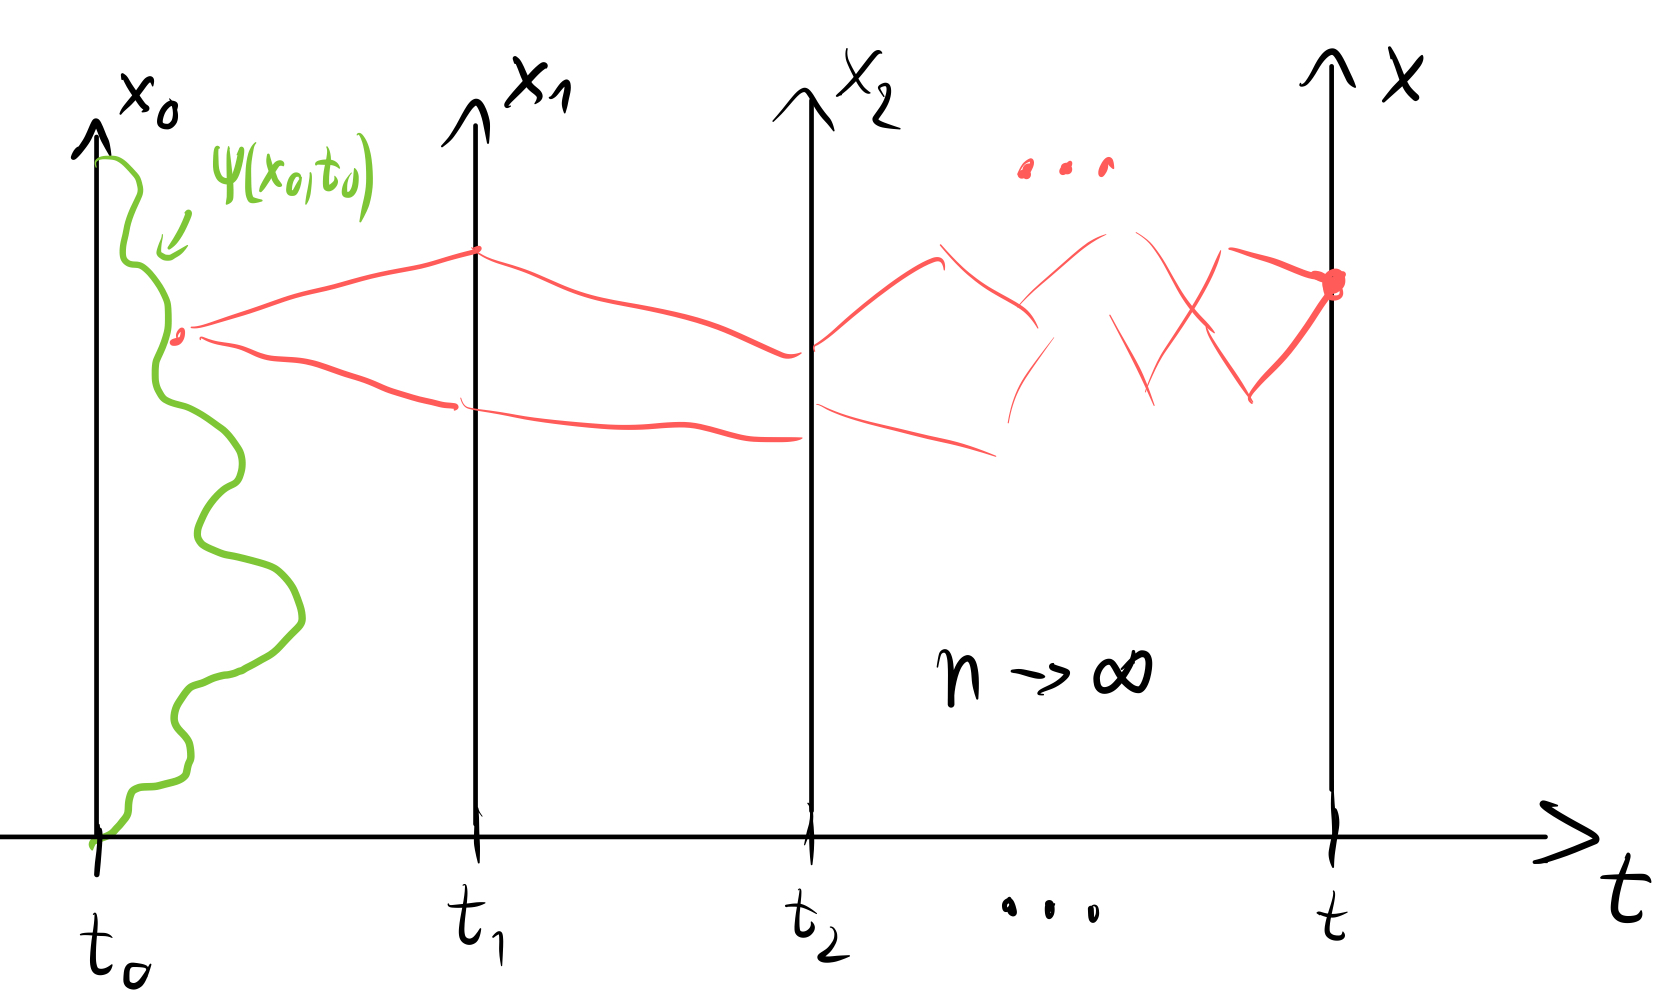
\includegraphics[width=0.8\linewidth]{Wyk_6_Rys_1.jpeg}
        \caption{Sumowanie po drogach dla cząstki kwantowej, liczona na propagatorach. Wyraża to też Feynmannowska \ind{Całka po trajektoriach}}
        \label{fig:lec_6:sumowanie}
\end{figure}

\section{\ind{Całka po trajektoriach}}
Wprowadzone do Mechaniki Kwantowej przez Feynmanna, jest to inny sposób na wyprowadzenie propagatora.\\
Zauważamy:
\[
    K(x, t, x_0, t_0) = \SumInt_{x(\tau)\footnotemark, x(t_0) = x_0, x(t) = t} f\qty[x(\tau)]
\]
\footnotetext{Trajektoria}
Intuicja: wiemy, że klasyczna trajektoria $\bar{x}(\tau)$ ekstremalizuje działanie:
\[
    S [x(\tau)] = \int_{t_0}^t \dd{\tau} L(\dot{x}(\tau), x(\tau))\qc L(\dot{x}, x) = \frac{m \dot{x}^2}{2} - V(x)
\]
Gdzie $L$ - Lagrangian. Weźmy więc $$f\qty[x(\tau)] = e^{\frac{i S [x(\tau)]}{\hbar}}$$
Dzięki temu w pobliżu trajektorii klasycznej będzie konstruktywna interferencja tych amplitud które sumujemy. Chcemy uzyskać taki efekt, żeby to się zgadzało z obserwowanym światem - zachowującym się klasycznie na skali makro.

\emph{Wniosek}: Wynika z tego fakt, że możemy wyprowadzić Mechanikę Kwantową wyprowadzić z Mechaniki Klasycznej!

Chcemy pokazać, że tak skonstruowany propagator daje nam $\Psi(x, t)$ spełniającą równanie Schrödingera. Rozważamy teraz infintezymalny czas $4 = t_0 + \epsilon$, $K(x, t_0+\epsilon, x_0, t_0) \stackrel{\epsilon \to 0}{\approx} $const., $$e^{1/\hbar \epsilon L(\frac{x - x_0}{\epsilon}, \frac{x+x_0}{2})}$$
Wtedy przeewoluowana funkcja falowa:
\[
    \Psi(x, t_0+\epsilon) = const. \int \dd{x_0} \Psi(x_0, t)e^{\frac{1}{\hbar} \qty(\frac{m(x - x_0)^2}{2\epsilon} - \epsilon V\qty(\frac{x+x_0}{2}))}
\]
Niech $\eta = x- x_0$, które jest małe i będziemy chcieli je rozwijać w $\epsilon$ i $\eta$, przy czym wkład do wyrażenia dadzą tylko $\eta \sim \sqrt{\epsilon}$. Wtedy:
\[
    \Psi(x, t_0) + \epsilon \pdv{t} \Psi(x, t)\eval_{t = t_0} \approx -const \int \dd{\eta} e^{\frac{i m \eta^2}{2 \hbar \epsilon}} \qty[\Psi(x, t_0) - \eta \pdv{x} \Psi(x, t_0) \frac{\eta^2}{2} \pdv[2]{x}\Psi] \qty[1 - \frac{i \epsilon}{\hbar} V(x - \frac{\eta}{2})]
\]
Pamiętajac o takiej przyjemnej własności:
\color{BrickRed}
\[ \int \dd{x} x^n e^{-ax^2} = \begin{cases}
    0\qq{dla nieparzystych}\\
    \frac{\sqrt{\pi}}{2^{n/2}} \cdot \frac{(n-1)!!}{a^{(n+1)/2}}\qq{dla parzystych}
\end{cases}
\]
\color{black}
\[
    \Psi(x, t_0) + \epsilon \pdv{t} \Psi(x, t)\eval_{t = t_0} \approx -const \qty[\Psi(x, t_0)\cdot \sqrt{\frac{\pi}{\frac{-im}{2 \hbar \epsilon}}} + \frac12 \pdv[2]{x} \Psi(x, t_0) \cdot \frac{\sqrt{\pi}}{2}\qty(\frac{-2\hbar\epsilon}{i m})^{\frac32}]\qty[1 - \frac{i \epsilon}{\hbar} V(x)]
\]
W najniższym rzędzie w $\epsilon$:
\[
    \Psi(x, t_0) = - const \Psi(x, t_0) \sqrt{\frac{2 \pi \hbar \epsilon}{- i m}}
\]
Co pozwala nam wyznaczyć stałą $const$. Będzie ona miała interpretację miary przy całkach po trajektoriach. 
\[
    \implies 
\]
Zmierzamy do równania Schrödingera. \com{Dopisz potem z ostatnich paru minut wykładu}
\end{lecture}

% ----------------------------------------------------------------------
% Wykład 23.03.2022


\begin{lecture}{Zasady nieoznaczoności}
\section{Off to propagator once more}
    Jak pamiętamy propagator zdefiniowaliśmy jak w równaniu \eqref{eq:lec_5:propagator}, tj.
    \[
        K(x, t, x_0, t_0) = const \sum_{x(\tau)} e^{iS[x(\tau)]} = \int D\qty[x(\tau)] e^{i S[x(\tau)]}\qq{, gdzie } S\qty[x(\tau)] = \int_{t_0}^t \dd{\tau} L(\dot{x}(\tau), x(\tau))\footnote{Gdzie $x(t_0) = x_0$ i $x(t) = x$}
    \]
    Weźmy sobie przykład, \ind{kwantowy oscylator harmoniczny}:
    \[
        V(x) = \frac12 m \omega^2 x^2\qc L = \frac{m \dot{v}^2}{2} - \frac12 m \omega^2 x^2
    \]
    Z tym, że zdefiniujmy sobie:
    \[
        x(\tau) = \bar{x}(\tau) + y(\tau)\qc 
        \mqty{\bar{x}(t_0) = x_0 & y(t_0) = 0\\
        \bar{x}(t) = x & y(t) = t}
    \]
    Wtedy nasz Lagrangian przyjmuje postać:
    \[
        L = \frac{m (\bar{x} + y)^2}{2} - \frac12 m \omega^2 (\bar{x} + y)^2 = \frac{m \dot{\bar{x}}^2}{2} - \frac12 m \omega^2 \bar{x}^2 + \frac{m \dot{y}^2}{2} - \frac12 m \omega^2 y^2 + m \dot{\bar{x}} \dot{y} - m \omega^2 \bar{x} y
    \]
    Dlatego działanie by wyglądało:
    \[
        S[x(\tau)] = S[x(\tau)] + S[y(\tau)] + \underbrace{\int_{t_0}^t \dd{\tau} m \dot{\bar{x}} \dot{y} - m \omega^2 \bar{x} y}_{\int_{t_0}^t \dd{t} \qty\underbrace{[- \dv{t}(m \ddot{\bar{x}} - m \omega^2 \bar{x})]}_{=0\footnotemark}y}
    \]
    \footnotetext{Klasyczne równanie ruchu}
    Odwołujemy się tu do wyprowadzenia równań Eulera-Lagrange'a:
    \[
        \dv{t} \dv{L}{\dot{x}} - \pdv{L}{x} = 0\qc\int_{t_0}^t \dd{\tau} \pdv{L}{\dot{x}} \delta \dot{x} + \pdv{L}{x} \delta\dot{x} = \footnote{Przez części} \int \dd{\tau} \underbrace{\qty[\qty(- \dv{t} \pdv{L}{\dot{x}}) + \pdv{L}{x}]}_{=0} \delta{x}
    \]
    Czyli efektywnie sobie rozdzielamy trajektorię klasyczną (do której w granicy skali makro będzie zbiegać nasza trajektoria) od trajektorii kwantowej, do której stosujemy całkę po trajektoriach
    \[
        K(x, t, x_0, t_0) = \exp(i \int_{t_0}^t \dd{\tau} L(\dot{\bar{x}}, \bar{x})) \cdot \int D\qty[y(\tau)] \exp(i \int_{t_0}^t \dd{\tau} L(\dot{y}, y))
    \]
    Czyli:
    \[
        K(x, t, x_0, t_0) = f(t, t_0) \exp(i \int_{t_0}^t \dd{\tau} L(\dot{\bar{x}}, \bar{x}))\footnote{Działanie na klasycznej trajektorii, zależność tylko od $x$, $x_0$}
    \]
    Gdzie klasyczna trajektoria oscylatora harmonicznego wygląda:
    \[
        \bar{x}(\tau) = \bar{x}(t_0) \cos(\omega\tau - t_0) + \frac{\dot{\bar{x}}(t_0)}{\omega} \sin(\omega \tau - t_0)\qc\dot{\bar{x}}(\tau) = - \omega \bar{x}(t_0) \sin(\omega \tau - t_0) + \dot{\bar{x}}(t_0) \cos(\omega \tau - t_0)
    \]
    A działanie:
    \[
        S\qty[\bar{x}(\tau)] = \int_{t_0}^t \dd{\tau}\qty( \frac{m \dot{\bar{x}}^2(\tau)}{2} - \frac12 m \omega^2 \bar{x}^2(\tau)) = \dots = h(\bar{x}(t_0), \dot{\bar{x}}(t_0), t, t_0)
    \]
    Co po wyrażeniu $\dot{x}(t_0)$ poprzez $\bar{x}(t_0) = x_0$ i $\bar{x}(t) = x$:
    \[
    \implies \dot{\bar{x}}(t_0) = \frac{\bar{x}(t) - \bar{x}(t_0) \cos \omega (t - t_0)}{\sin \omega (t - t_0)} \cdot \omega = \omega \cdot \frac{x - x_0\cos\omega(t - t_0)}{\sin \omega (t - t_0)}
    \]
    Co po wstawieniu do $h$ daje:
    \[
        S[\bar{x}(\tau)] = \frac{m \omega}{2 \sin\qty[\omega (t-t_0)]} \qty[(x^2 + x_0^2) \cos\omega(t-t_0) - 2 x x_0]
    \]
    I wstawieniu wyżej:
    \[
        K(x, t, x_0, t_0) = f(t, t_0) \exp\qty(\frac{m \omega}{2 \sin\qty[\omega (t-t_0)]} \qty[(x^2 + x_0^2) \cos\omega(t-t_0) - 2 x x_0])
    \]
    Zaś aby wyznaczyć $f(t, t_0)$ wystarczy przepropagować dowolny stan (np. gaussowski) i należy nałożyć watunek zachowania normalizacji. Tym sposobem uciekamy od problemu całki po trajektoriach i dostajemy wynik:
    \[
        f(t, t_0) = \sqrt{
        \frac{m \omega
        }{2 \pi i \hbar \sin\omega(t-t_0)
        }}
    \]
    Co po wzięciu $\omega\to0$ powinno nam odtworzyć propagator dla cząstki swobodnej:
    \[
        K_{\omega = 0}(x, t, x_0, t_0) = \sqrt{\frac{m}{2 \pi i \hbar(t-t_0)}}
    \]
    
    \section{Zasada niezoaczoności Heisenberga-Robertsona}
    Przypomnijmy sobie paczkę Gaussowską:
    \[
        \Psi(x) = \frac{1}{(2 \pi \sigma^2)^{\frac14}} e^{- \frac{(x - x_0)^2}{4 \sigma^2} + \frac{i p_0 x}{\hbar}}
    \]
    A na ćwiczeniach wyszło nam dla paczki Gaussowskiej:
    \[
        \mqty{\Delta^2 x = \sigma^2 \\
        \Delta^2 p = \frac{\hbar^2}{4 \sigma^2}}
    \]
    Czyli im lepiej określone położenie, tym gorzej określony pęd. Daje to znaną postać \subind{Zasady nieoznaczoności Heisenberga}{Zasada Nieoznaczoności!Heisenberga}:
    \begin{equation}
        \Delta^2 x \Delta^2 p \geq \frac{\hbar^2}{4}
        \label{eq:lec_7:heisenberg}
    \end{equation}
    Co jest szczególnym przypadkiem zasady sformułowanej dla dowolnych dwóch niekomutujących obserwabli $\hat{A}, \hat{B}$ i stanu $\ket{\Psi}$.
    \subsection{Twierdzenie}
    \[
        \underbrace{\Delta^2 A}_{\ev{\hat{A}^2}{\Psi} - \ev{\hat{A}}{\Psi}^2} \cdot \Delta^2 B \geq \frac14 |\underbrace{\ev{[A, B]}}_{\ev{[A, B]}{\Psi}}|
    \]
    W szczególności"
    \[
        \hat{A} = \hat{x} \qc \hat{B} = \hat{p} \qc [\hat{x}, \hat{p}] = i \hbar \implies \Delta^2 x \Delta^2 p \geq \frac{\hbar^2}{4}
    \]
    Czyli stan Gaussowski wysyca zasadę nieoznaczoności
    \subsection{Dowód}
    Niech:
    \[
        \mqty{
        \hat{A}' = \hat{A} - \ev{\hat{A}}\cdot\Id \\
        \hat{B}' = \hat{B} - \ev{B}\cdot \Id}
        \implies
        \mqty{
        \ev{\hat{A}'} = 0 & \Delta^2 A' = \Delta^2 A\\
        \ev{\hat{B}'} = 0 & \Delta^2 B' = \Delta^2 B
        }
    \]
    Teraz zdefiniujmy sobie operator $\hat{F} = \hat{A}' + i \lambda \hat{B}', \lambda \in \mathbb{R}$.\\
    {\color{BrickRed} Rozważmy $F^\dagger F$ - ten operator (jest on \emph{Dowolny}) jest hermitowski i dodatni, bo $\forall_{\ket{\Psi}} \ev{F^\dagger F}{\Psi} \geq 0$}
    W związku z tym możemy sobie zapisać:
    \[
        \forall_{\ket{\Psi}} \mqty{
        \ev{(\hat{A}' - i \lambda \hat{B}')(\hat{A}' + i \lambda \hat{B}')}{\Psi} \geq 0\\
        \ev{\hat{A}'^2 + \lambda^2\hat{B}'^2 + i \lambda (\hat{A}'\hat{B}' - \hat{B}'\hat{A}')} \geq 0
        }
    \]
    Co daje nam:
    \[
        \mqty{
        \Delta^2A' + \lambda^2 \Delta^2 B' + i \lambda \ev{[A', B']} \geq 0\\
        \Delta^2 A + \lambda^2 \Delta^2 B + i \lambda \ev{[A, B]} \geq 0\\
        }
    \]
    Co jest prawdziwe dla dowolnej $\lambda$, czyli $\Delta = b^2 - 4 a c \leq 0$, co daje:
    \[
        \underbrace{\qty(\underbrace{i \overbrace{\ev{[A, B]}}^{\text{czysto urojone}}}_{\text{czysto rzeczywiste}})^2}_{dodatnie} - 4 \Delta^2A\Delta^2B \leq 0
    \]
    Czyli pamiętając, że $\ev{[A, B]}^\ast = - \ev{[A, B]}$ finalnie dostajemy dowód na nierówność:
    \begin{equation}
        \Delta^2 A \Delta^2 B \geq \frac14 \qty|\ev{\comm{A}{B}}|
        \label{eq:lec_7:heisenberg_robertson}
    \end{equation}
    
    {\color{SeaGreen}Z tym, że mamy nie myśleć o tym jak Heisenberg, że pomiar jednego zaburza drugie, a że nie ma stanów kwantowych w których wariancje obu obserwabli są jednocześnie małe.}
\end{lecture}

% --------------------------------------------------------
% Wykład 25.03.2022

\begin{lecture}{Zasady nieoznaczoności C.D.}
    Na ostatnim wykładzie wyprowadzilliśmy sobie ogólną zasadę nieoznaczoności Heisenberga - Robertsona. Ma postać jak w równaniu \eqref{eq:lec_7:heisenberg_robertson}:
    \[
        \Delta^2 A \Delta^2 B \geq \frac14 \qty|\ev{\comm{A}{B}}|
    \]
    \section{Jednoczesny pomiar komutujących obserwabli}
    {\color{Orange} Fakt:} Jeśli $\comm{A}{B} = 0$, to możliwy jest jednoczesny pomiar $\hat{A}$ i $\hat{B}$.\\
    {\color{Emerald} Dowód:} Chcemy pokazać, że istnieje baza ortonormalna $\qty{\ket{a_i, b_j}}$ taka, że $\hat{A}\ket{a_i, b_j} = a_i \ket{a_i, b_j}, \hat{B} \ket{a_i, b_j} = b_j \ket{a_i, b_j}$ (Wspólna baza wektorów własnych $\hat{A}$ i $\hat{B}$.)\\
    Niech $\ket{a_i} \ket{a_2}$ będą wektorami własnymi $\hat{A}$, wtedy: $\mqty{\hat{A} \ket{a_1} = a_1 \ket{a_1} \\
    \hat{A} \ket{a_2} = a_2 \ket{a_2}}$. Ale wtedy wiemy też, że $\comm{\hat{A}}{\hat{B}} = 0$, czyli:
    \begin{align*}
        \mel{a_1}{\comm{\hat{A}}{\hat{B}}}{a_2} =& 0\\
        \mel{a_1}{\hat{A}\hat{B} - \hat{B}\hat{A}}{a_2} =& 0\\
        \underbrace{\mel{a_1}{\hat{A}\hat{B}}{a_2}}_{\bra{a_1}a_1} - \underbrace{\mel{a_1}{\hat{B}\hat{A}}{a_2}}_{a_2\ket{a_2}} &= 0
    \end{align*}
    Czyli:
    \[
        (a_1 - a_2)\mel{a_1}{\hat{B}}{a_2} = 0
    \]
    I dzieje się tak dla dowolnych $\ket{a_i}$. Jeśli wszystkie $a_i$ są od siebie różne (Czyli $\hat{A}$ nie jest zdegenerowane) to mamy:
    \[
        (a_i - a_j) \mel{a_i}{\hat{B}}{a_j} = 0 \implies \mel{a_i}{\hat{B}}{a_j} = \delta_{ij}\mel{a_i}{\hat{B}}{a_i}
    \]
    Czyli dostajemy, że $\hat{B}$ jest diagonalny w bazie własnej $\hat{A}$.\\
    Jeśli mamy degenerację, czyli $\forall i \in S_a, a_i = a \implies$ {\color{WildStrawberry} B ma postać \emph{blokowo diagonalną}, z każdym blokiem nad podprzestrzenią $\HS_a = \ev{\ket{a_i}, \ket{a_j}}$, a operator $\hat{A}$ nad przestrzenią $\HS_a$ działa jak $a \cdot \Id_{\HS_a}$.}\\
    Czyli wynika z tego, że {\color{Plum} Możemy ramach bloku zdiagonalizować $\hat{B}$ nie zmieniając postaci $\hat{A}$ (Bo $U_a \Id_{\HS_a} U^\dagger = \Id_{\HS_a}$)}.\\
    Czyli istnieje baza własna $\ket{a_i, b_j}$ taka, że $\mqty{
    \hat{A}\ket{a_i, b_j} = a_i \ket{a_i, b_j}\\
    \hat{B}\ket{a_i, b_j} = b_j \ket{a_i, b_j}}$ 
    
    {\color{Magenta} Wniosek:} Jeśli mamy więcej komutujących obserwabli $\hat{A}, \hat{B}, \hat{C}, \dots$, to możemy skonstruować bazę \\ $\ket{a_i, b_j, c_k, \dots}$ taką, że $\mqty{\hat{A}\ket{a_i, b_j, c_k, \dots} = a_i \ket{a_i, b_j, c_k, \dots}\\
    \hat{B} \ket{a_i, b_j, c_k, \dots} = b_j \ket{a_i, b_j, c_k, \dots}\\
    \hat{C} \ket{a_i, b_j, c_k, \dots} = c_k \ket{a_i, b_j, c_k, \dots}\\ \dots}$
    {\color{Orange} Definicja:} Jak wartości własne jednocznacznie identyfikują jako wektor $\ket{a_i, b_j, c_k, \dots}$ \com{Zdj od Krzyśka}
    
    \section{Jednoczesny pomiar niekomutujących obserwabli (?)}
    Niech $\comm{A}{B} \neq 0$, to {\color{red}nie istnieje baza własna}.
    Dowód a.a.\\
    Gdyby istniała baza ortogonalna $\mqty{
    \hat{A}\ket{a_i, b_j} = a_i \ket{a_i, b_j}\\
    \hat{B}\ket{a_i, b_j} = b_j \ket{a_i, b_j}} \implies \mel{a_i, b_j}{\comm{\hat{A}}{\hat{B}}}{a_i', b_j'}$ = $\qty(a_i b_j - a_{i'} b_{j'}) \delta_{jj'}\delta_{ii'}$ $= 0 \implies \comm{\hat{A}}{\hat{B}} = 0$ {\color{red}sprzeczność}.\\
    Niemniej, mimo to można pytać się  o jednoczesny (ale rozmyty) pomiar niekomutujących obserwabli, np.$\hat{x}, \hat{p}$. Intuicja:
    \begin{align*}
        \Psi_{x_0, p_0} = \frac{1}{(2 \pi \sigma^2)^{\frac14}} \exp &\qty(- \frac{(x-x_0)^2}{4 \sigma^2} + \frac{i p_0 x}{\hbar})\\
        \ev{\hat{x}} = x_0 &\qc \Delta^2 x = \sigma^2\\
        \ev{\hat{p}} = p_0 &\qc \Delta^2 p = \frac{\hbar}{4\sigma^2}
    \end{align*}
    Ten stan ma jednoznacznie określone położenie i pęd najlepiej jak się da, bo: 
    \[
        \Delta^2 x \Delta^2 p = \frac{\hbar^2}{4}
    \]
    (Czyli wysyca \subind{zasadę nieoznaczoności Heisenberga-Robertsona}{Zasada Nieoznaczoności!Heisenberga-Robertsona}), gdzie $\ket{x_0, p_0}$ - stan odpowiadajacy $\Psi_{x_0, p_0}$. Czyli moglibyśmy stworzyć "siatkę" stanów o w miarę dobrze określonych $\hat{x}$ i $\hat{p}$, który byłyby prawie ortogonalne i moglibysmy to traktować jako bazę pomiarową.\\
    Jeśli tak myślimy, to dostajemy wynik mówiący o położeniu cząstki z precyzją $\delta^2 x = \sigma^2$, $\delta^2p = \frac{\hbar^2}{4 \sigma^2}$.\\
    Jeśli mamy jakiś stan $\ket{\phi}$, którego w ten sposób mierzymy położenia z rozrzutem
    \[
    \Delta^2 x' = \underbrace{\Delta^2}_{\footnotemark} x + \underbrace{\delta^2}_{\footnotemark} x, \Delta^2p' = \Delta^2 p + \delta^2 p
    \]
    \addtocounter{footnote}{-1}
    \footnotetext{Wariancja dla idealnego pomiaru położenia}
    \refstepcounter{footnote}
    \footnotetext{Wariancja rozmycia 'linijki' którą mierzymy}
    Możemy teraz napisać \subind{zasadę nieoznaczoności dla łącznego pomiaru}{Zasada Nieoznaczoności!łącznego pomiaru}$\hat{x}, \hat{p}$ (tak jak chciał Heisenberg).
    \[
        \Delta^2 x' \Delta^2 p' = \underbrace{\Delta^2x\Delta^2p}_{\geq \frac{\hbar^2}{4}} + \underbrace{\delta^2x\delta^2p}_{\geq \frac{\hbar^2}{4}} + \Delta^2x\delta^2p + \delta^2x\Delta^2p \geq \frac{\hbar^2}{4} + \frac{\hbar^2}{4}\underbrace{\qty(\frac{\Delta^2 x}{\delta^2 x} + \frac{\delta^2 x}{\Delta^2 x})}_{x+\frac{1}{x} \geq 2}
    \]
    Co daje nam finalnie:
    \begin{equation}
        \Delta^2 x' \Delta^2 p' \geq \hbar^2
        \label{eq:lec_8:heisenberg_full}
    \end{equation}
    
    \section{Zasada niezoznaczoności czas-energia \com{Dodaj indeks}}
    $\hat{\HS}$ - operator energii, ale nie mamy operatora czasu $\hat{t}$, czyli nie możemy używać zasady nieoznaczoności Heisenberga-Robertsona, ale spodziewamy się, że coś podobnego powinno być, bo szybkość ewolucji stanów jest związana z rozrzutem Energii ($\Delta^2 \HS$)
\end{lecture}


% ------------------------------------------------------------------------
% 30.03.22

\begin{lecture}{\subind{Potencjał Kwadratowy}{Potencjał!Kwadratowy}}
    \section{Off to zasady nieoznaczoności once more}
    Na ostatnim wykładzie sobie powiedzieliśmy, że jest zasada nieoznaczoności czas-energia. Mówimy sobie tutaj, że propagacja błędu jest \emph{liniowa}, co pozwala nam na wyliczenie niepewności estymacji czasu na podstawie pomiaru $\hat{A}$. Wtedy niepewność pomiaru czasu naszego estymatora to:
    \[
        \Delta^2 t = \frac{\Delta^2 \hat{A}}{\abs{\dv{\ev{A}_t}{t}}^2}
    \]
    Chcąc wyznaczyć niepewność czasu z zasady heisenberga-robertsona musimy użyć tricku, bo explicite nie da się stamtąd czasu wyznaczyć. Ale już dla dowolnej obserwabli której wartość oczekiwana zależy od czasu już to zadziała, więc to dokładnie robimy. Pamiętająco tym, że $\psket{t} = e^{-i\hat{\HS}t /\hbar} \psket{0}$ możemy sobie zapisać:
    \begin{equation}
        \dv{\ev{\hat{A}}_t}{t} = - \frac{i}{\hbar} \ev{\comm{\hat{A}}{\hat{\HS}}}
        \label{eq:lec_9:A_od_t}
    \end{equation}
    Możemy teraz to wstawić do standardowej zasady nieoznaczoności \eqref{eq:lec_7:heisenberg_robertson}, gdzie obserwabla $\hat{\mathrm{B}} = \hat{H}$:
    \[
        \Delta^2t \geq \frac{1}{\abs{\dv{\ev{A}_t}{t}}^2} \cdot \frac{\frac14\ev{\comm{\hat{A}}{\hat{H}}}^2}{\Delta^2 H} \stackrel{\eqref{eq:lec_9:A_od_t}}{=} \frac{\hbar^2}{4 \Delta^2\hat{H}} \implies
    \]
    \begin{emph_box}{\subind{Zasada nieoznaczoności czas-energia}{Zasada Nieoznaczoności!czas-energia}}
    \begin{equation}
        \Delta^2 t \Delta^2\hat{H} \geq \frac{\hbar^2}{4}
        \label{eq:lec_9:nieoznaczonosc_czas_energia}
    \end{equation}
    \end{emph_box}
    
    \section{Kwantowy Oscylator Harmoniczny}
    Dla kwantowego oscylatora harmonicznego mamy Hamiltonian:
    \[
        \hat{H} = \frac{\hat{p}^2}{2m} + \frac12 m \omega^2 \hat{x}^2
    \]
    {\color{TealBlue}
    Co położeniowo by miało reprezentację:
    \[
        \hat{H} = - \frac{\hbar^2}{2m} \dv[2]{x} + \frac12 m \omega^2 \hat{x}^2
    \]
    Co aby rozwiązać musielibyśmy rozwiązać problem własny, tj. \eqref{eq:lec_5:schrodinger_bez_czasu} co dało by nam energie własne $E$ i odpowiadające im stany własne $\Psi_E(x)$
    }
    Rozwiązując ten problem podejdziemy do tego algebraicznie. Zdefiniujemy sobie dwa operatory:
    \begin{emph_box}{\subind{Operatory kreacji i anihillacji}{Operator!Kreacji}\index{Operator!Anihillacji}}
    \emph{Operator kreacji}
        \begin{equation}
            \hat{a} = \sqrt{\frac{m \omega}{2 \hbar}}\qty(\hat{x} + \frac{i \hat{p}}{m \omega})
            \label{eq:lec_9:operator_anihillacji}
        \end{equation}
        \emph{Operator anihillacji}
        \begin{equation}
            \hat{a}^\dagger = \sqrt{\frac{m \omega}{2 \hbar}}\qty(\hat{x} - \frac{i \hat{p}}{m \omega})
            \label{eq:lec_9:operator_kreacji}
        \end{equation}
        Mają one przyjemną własnośc taką, że $\comm{a}{a^\dagger} = 1\footnotemark$\\
        \textbf{Cytat z Demko: operator $a$ jak knihillacji, a $a^\dagger$ krzyż jak kreacji}
    \end{emph_box}
    \footnotetext{Patrz Wyprowadzenie \ref{fig:app_9:comm_kreacji_anihillacji}}
    Zauważamy teraz, że:
    \[
        a a^\dagger = \frac{m \omega}{2 \hbar} \qty(\hat{x} - \frac{i \hat{p}}{m \omega})\qty(\hat{x} + \frac{i \hat{p}}{m \omega}) = \frac{m\omega}{2\hbar} \hat{x}^2 + \frac{\phat^2}{2 \hbar m \omega} - \frac12
    \]
    Czyli widzimy, że:
    \[
        \hat{H} = \hbar \omega\qty(\hat{a}\hat{a}^\dagger + \frac12)
    \]
    Co oznacza, że szukamy stanów własnych $\hat{H}$, co jest równoważne szukaniu stanów własnych $\hat{a}\hat{a}^dagger$. W związku z tym możemy sobie oznaczyć $\hat{n} = \hat{a}\hat{a}^dagger$.
    \subsection{Szukanie stanów własnych i wartości własnych $\hat{n}$}
    Niech $\ket{n}$ będzie stanem własnym $\hat{n}$ o wartości własnej $n$:
    \[
        \hat{n} \ket{n} = n \ket{n}
    \]
    Teraz rozważmy sobie stan nieunormowany $\ket{\xi} = \hat{a} \ket{n}$ i rozważmy działanie $\hat{n}$ na $\ket{\xi}$. Dostaniemy, że:
    \[
        \hat{n} \ket{\xi} = (n-1)\ket{\xi}
    \]
    Czyli $\hat{a}\ket{n}$ jest też stanem własnym $\hat{n}$ o wartości własnej $(n-1)$.\\
    W ten sposób stwierdzamy, że $a^k \ket{n}$ będzie wektorem własnym nieunormowanym o wartości własnej $n-k$\footnote{Patrz wyprowadzenie \ref{fig:app_9:stany_wlasne_n}} ($k\in\mathbb{N}$).\\
    Spróbujmmy je teraz unormować. Zauważmy, że $\braket{\xi} = \ev{\hat{a}^\dagger\hat{a}}{n} = n \braket{n} = n$.\\
    Oznacza to, że unormowany stan własny $\ket{n - 1} = \frac{1}{\sqrt{n}} \hat{a} \ket{n}$ itd. czyli $\ket{n-k} = \frac{1}{\sqrt{n \cdot(n-1) \dots  (n-k+1)}} a^k \ket{n}$
    
    Ta konstrukcja urwała by się tylko jak $n \in \mathbb{N}$, bo dla $\hat{a}\ket{a} = 0$. W przeciwnym razie byśmy wygenerowali stany własne $\ket{n}$ o dowolnie ujemnym $n$.\\
    Ale zauważmy, że operator $\hat{n} = \hat{a}\hat{a}^\dagger$ jest operatorem dodatnim, czyli nie moze mieć wartości własnych ujemnych. Czyli jedyna możliwość to, że $n\in\mathbb{N}$. To oznacza, że mamy stan $\ket{0}$ taki, żę $\hat{a}\ket{0} = 0$ i zauważamy, że $\ket{n-1} = \frac{1}{\sqrt{n}} \hat{a} \ket{n} \implies a^\dagger\ket{n-1} = \frac{1}{\sqrt{n}} \hat{a}^\dagger \hat{a} \ket{n}$ co oznacza, że
    \[
        \hat{a}^\dagger \ket{n-1} = \sqrt{n}\ket{n}
    \]
    Co pokazuje działanie operatora kreacji, bo podnosi on wartość stałej normalizującej. Mamy również: $\ket{n} = \frac{1}{\sqrt{n}} a^\dagger \ket{n-1}\qc\ket{n+1} = \frac{1}{\sqrt{n+1}} \hat{a}^\dagger \ket{n}$\\
    Widzimy teraz, że znając stan $\ket{0}$ mamy wszystkie inne stany ze wzoru 
    \[
    \ket{n} = \frac{1}{\sqrt{n!}} \qty(\hat{a}^\dagger)^n\ket{0}
    \]
    To są stany własne $\hat{H} = \hbar \omega (\hat{a}\hat{a}^\dagger + \frac12) = \hbar \omega (\hat{n} + \frac12)$ z energią $E_n = \hbar \omega (n + \frac12)\qc n = 0, 1, 2, \dots$\\
    \begin{figure}[!ht]
        \centering
        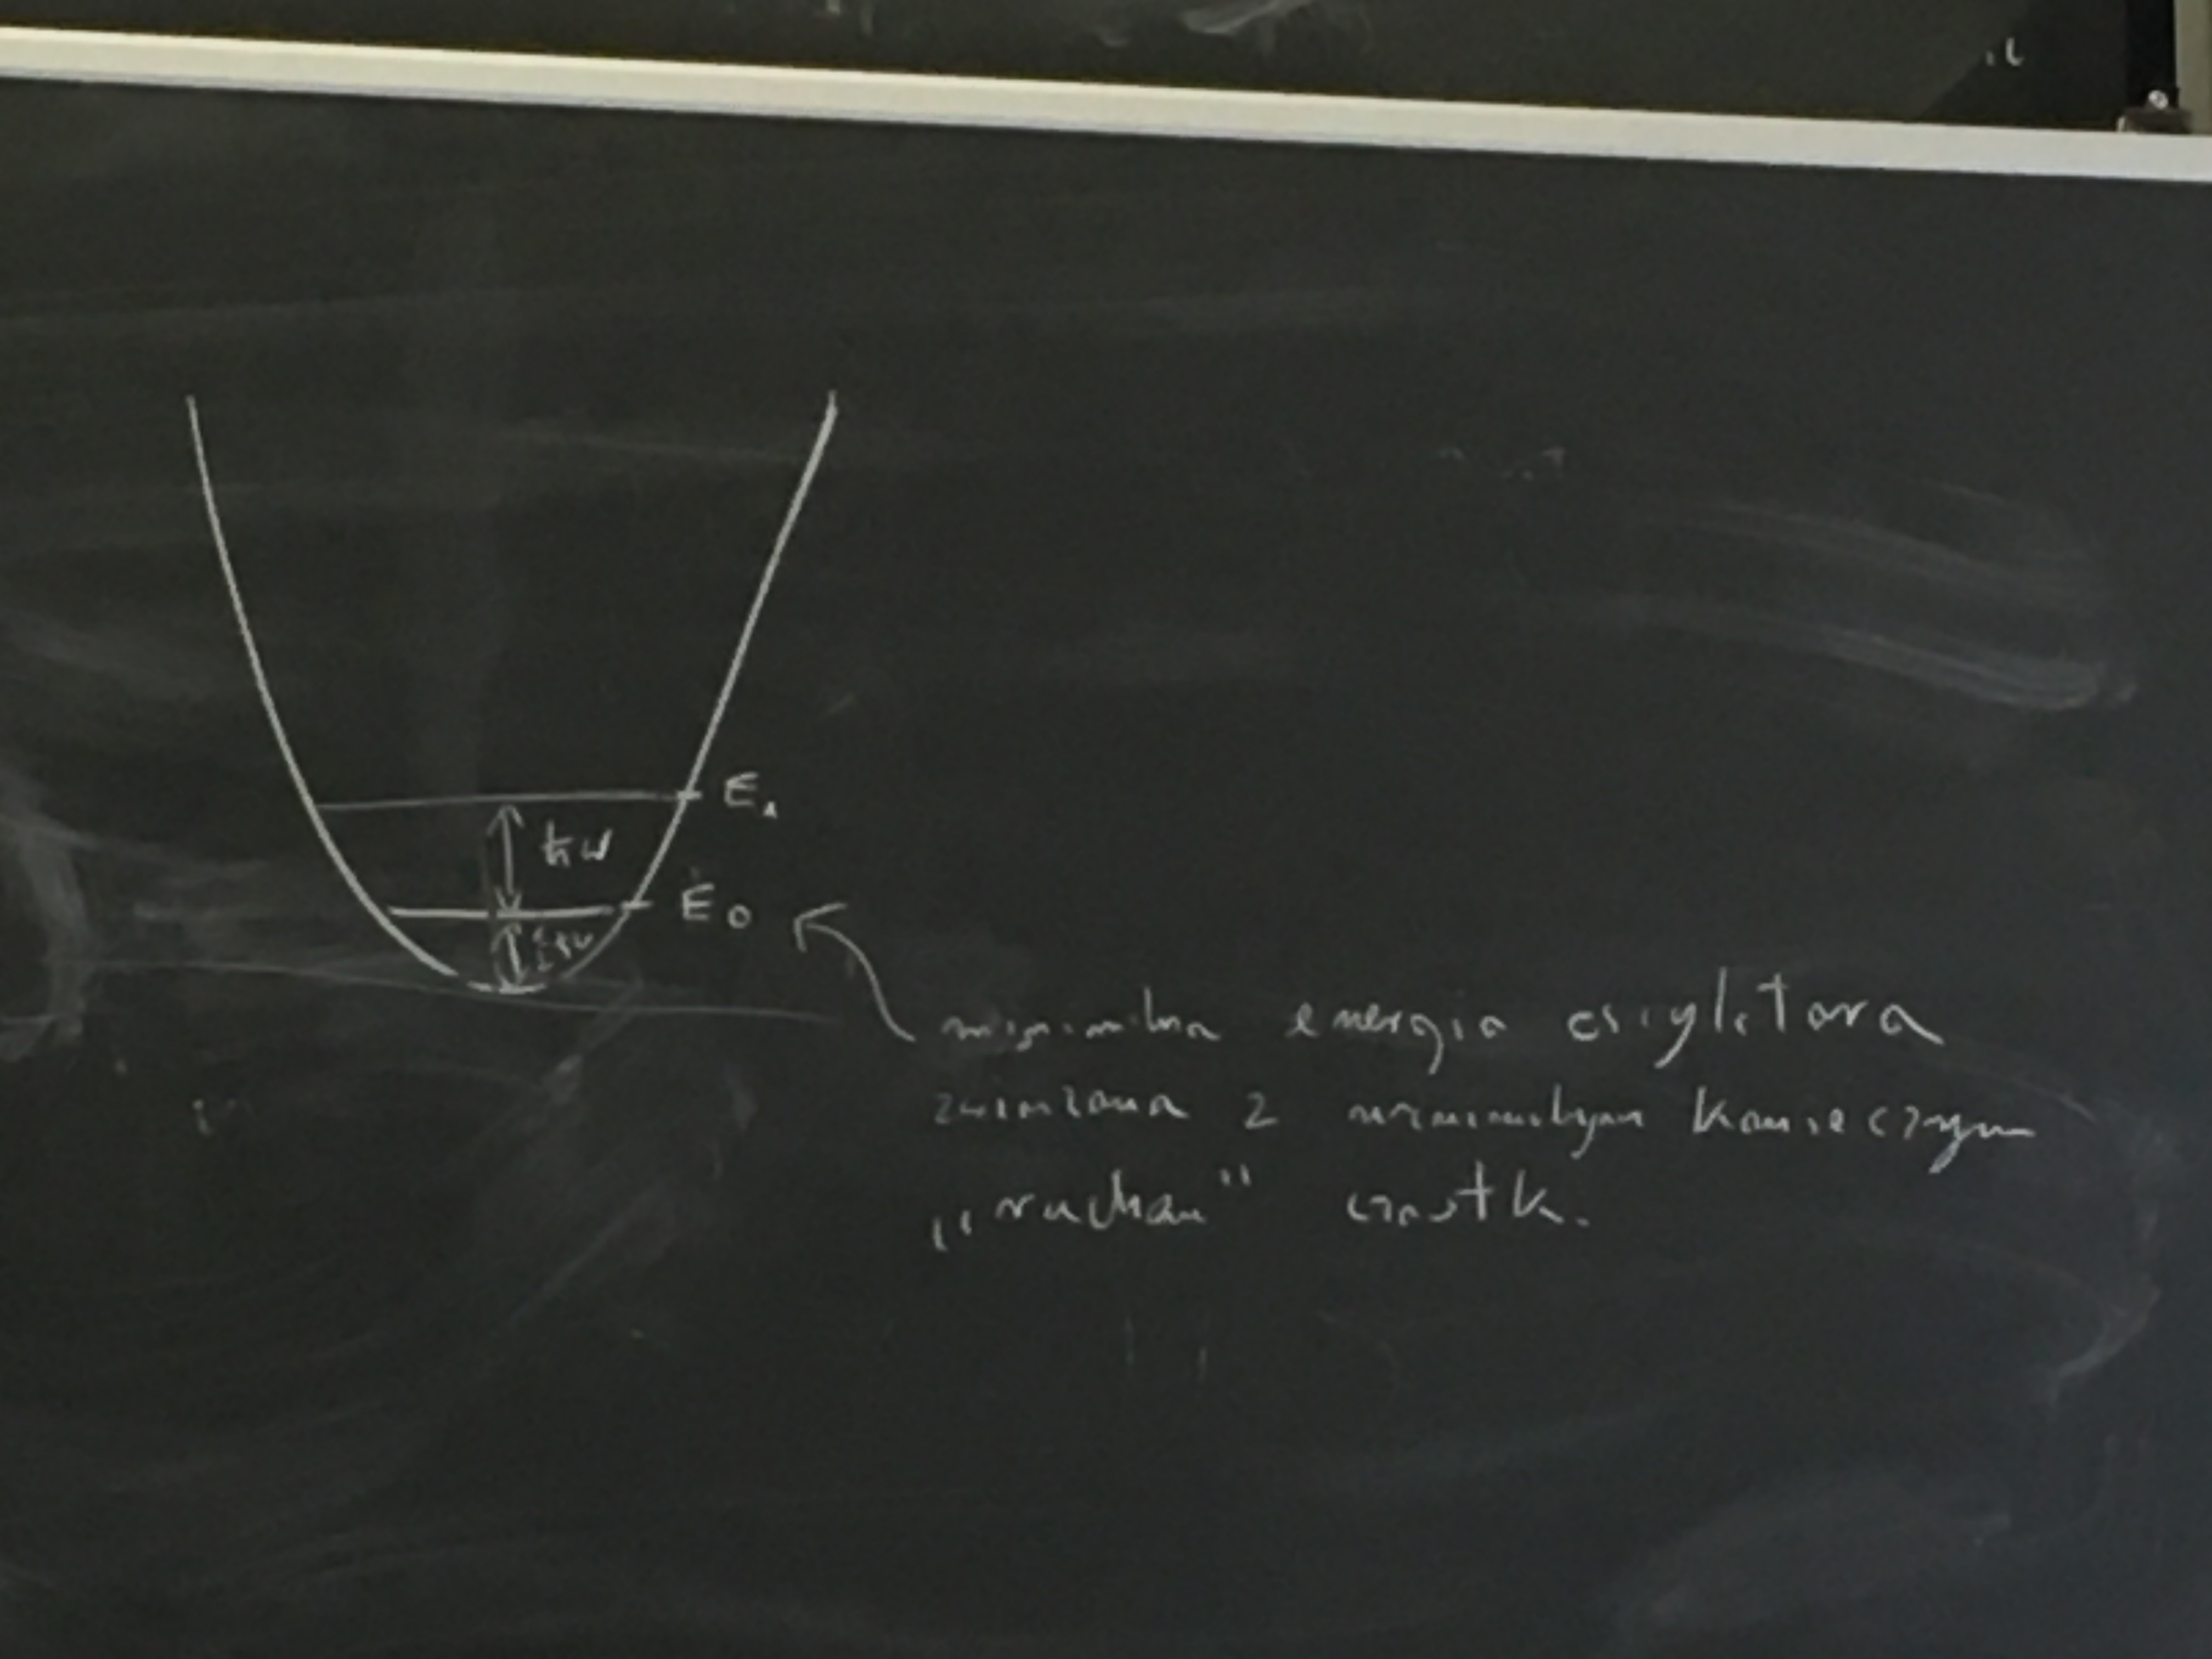
\includegraphics[width=\linewidth]{Wyk_9_Rys_1.JPG}
        \caption{Rysunek studni potencjału dla kwantowego oscylatora harmonicznego \com{Przerysuj i wstaw}}
        \label{fig:lec_9:studnia_osc}
    \end{figure}
    Teraz zobaczmy czym jest $\ket{0}$\\
    Zapiszmy warunek $\hat{a}\ket{0}$ w reprezentacji położeniowej:
    \[
        \sqrt{\frac{m \omega}{2 \hbar}} \qty(x + \frac{\hbar}{m\omega}\dd{x}) \Psi_0(x) = 0\qc\frac{\hbar}{m\omega} \dv{\Psi}{x} = - x \Psi \qc \frac{1}{\Psi} \dv{\Psi}{x} = - \frac{m\omega}{\hbar} x = \dd{x}(\ln \Psi)\qc \ln\Psi = - \frac{m\omega}{2\hbar} x^2 + C
    \]
    Czyli stan podstawowy:
    \[
        \Psi_0(x) = e^{- \frac{m\omega}{2 \hbar} x^2 + C} \approx A e^{- \frac{m\omega}{2 \hbar} x^2} \stackrel{\footnotemark}{=} \qty(\frac{m\omega}{\pi \hbar})^{\frac14} e^{- \frac{m\omega}{2 \hbar} x^2}
    \]
    \footnotetext{Normalizacja}
    Co daje nam Gaussa, o szerokości $\sigma = \sqrt{\frac{\hbar}{2 m \omega}}$ i fluktuacje $\xhat, \phat$ w stanie podstawowym:\\
    \[
        \Delta^2 x = \frac{\hbar}{2 m \omega}\qc\Delta^2p = \frac{\hbar m \omega}{2}
    \]
    I z tych fluktuacji daleko dalej będą wynikać bardzo fundamentalne wnioski, np to, że w próżni nie może być absolutne 'nic', ponieważ i tak będą się kreować i anihillować pola $E$ i $B$, żeby zasada nieoznaczoności Heisenberga była spełniona.
\end{lecture}

% --------------------------------------------------------
% Wykład 01.04.2022

\begin{lecture}{Prima Aprilis}
\section{W poprzednim odcinku...}
Zdefiniowaliśmy stany energetyczne $E_n = \hbar \omega (n+\frac12), n \in {0, 1, 2, \dots}$\\
Oraz operatory kreacji i anihillacji: 
$\ket{n} = \frac{1}{\sqrt{n}} (\hat{a}^\dagger)^n \ket{0}$, tj.:
\[
    \hat{a} \ket{n} = \sqrt{n} \ket{n-1}\qc\hat{a}^\dagger \ket{n} = \sqrt{n+1} \ket{n+1}
\]
Definiując po drodze jeszcze, że $\hat{a}\ket{0} = 0, \hat{a} = \sqrt{\frac{m \omega}{2 \hbar}} \qty(\hat{x} + \frac{i \phat}{m \omega})$\\
Zdefiniowalismy też stan podstawowy, który okazał się być funkcją Gaussa:
\[
    \Psi_0(x) = \qty(\frac{m \omega}{\pi \hbar})^{\frac14} e^{-\frac{m \omega}{2 \hbar} x^2}
\]
\section{Wyznaczanie kolejnych stanów $\Psi_n$}
Znając stan podstawowy $\Psi_0$ możemy sobie teraz zadań pytanie jak będa wyglądać kolejne stany wzbudzeń? Otóż stan $n$-ty zdefiniujemy jako:
\[
    \Psi_n(x) = \frac{1}{\sqrt{n!}}\qty[\sqrt{\frac{m \omega}{2 \hbar}} \qty(x - \frac{\hbar}{m \omega} \dv{x})]^n \qty(\frac{m \omega}{\pi k})^{\frac14} e^{-\frac{m \omega}{2 \hbar} x^2}
\]

Teraz zmieńmy zmienne na $q = \sqrt{\frac{m \omega}{\hbar}}x$ i po znormalizowaniu na nowo funkcji \com{Zdjęcie tego i rysunek stanów własnych} dostajemy:
\begin{equation}
    \Psi_n'(q) = \frac{1}{\sqrt{\sqrt{\pi} n! 2^n}} \underbrace{H_n}_{\footnotemark} \qty(q - \dv{q})^n e^{-\frac{q^2}{2}}
    \label{eq:lec_10:stany_n}
\end{equation}
\footnotetext{Pewien wielomian od $q$}
Gdzie ten wielomian okazuje się być wzorem z nazwiskiej, czyli jest to 
Wielomian Hermite'a:
\begin{emph_box}{\subind{Wielomiany Hermite'a}{Wielomiany!Hermite'a}}
    \begin{equation}
        H_n = e^{\frac{q}{2}} \qty(q - \dv{q})^n e^{-\frac{q^2}{2}}
        \label{eq:lec_10:wielomiany_hermita}
    \end{equation}
    W ogólności:
    \begin{itemize}
        \item dla n nieparzystych $H_n$ - wielomian nieparzysty $\implies \Psi_n(x) = -\Psi_n(-x)$ antysymetryczne
        \item dla n parzystych $H_n$ - parzysty $\implies \Psi_n(x) = \Psi_n(-x)$
    \end{itemize}
\end{emph_box}
\subsection{Własności wielomianów Hermite'a}
    Pierwsze kilka tych wielomianów to:
    \begin{align*}
        H_0(q) &= 1\\
        H_1(q) &= 2q\\
        H_2(q) &= 4q^2 - 2\\
        \dots
    \end{align*}
    Dalej, z ortogonalności $\Psi_n(x)$:
    \[
        \int_{-\infty}^{\infty}\dd{x} \Psi_n(x)^\ast \Psi_m(x) = \delta_{n,m} \implies \int_{-\infty}^{\infty} \dd{q} H_n(q) H_m(q) e^{-q^2} = \delta_{n,m} 
    \]
    Czyli Wielomiany Hermite'a też \subind{są ortogonalne!}{Ortogonalność}
    \section{Stany Koherentne}
    Chcielibyśmy znaleźć stany, które by w pewnucm przybliżeniu reprezentowały klasyczny ruch w oscylatorze harmonicznym. Takie stany to właśnie \subind{stany koherentne}{Stany!Koherentne}. \\
    {\color{Orange} Definicja:} Stanem koherentnym nazywamy unormowane stany własne operatora anihillacji:
    \[
        \hat{a}\ket{\alpha} = \alpha \ket{\alpha}
    \]
    Widzimy z tego równania, że $\alpha$ to wartość własna, która może być zespolona, a $\ket{alpha}$ to unormowany stan własny.\\
    {\color{teal} Fakt}:
    \[
        \ket{\alpha} = e^{- \frac{\abs{\alpha}^2}{2}} \sum_{n=0}^{\infty} \frac{\alpha^n}{\sqrt{n!}} \ket{n}
    \]
    {\color{Emerald} Dowód:}
    \[
        \braket{\alpha} = e^{- \abs{\alpha}^2} \sum_{n,m} \frac{(\alpha^\ast)^n}{\sqrt{n!}}\frac{\alpha^n}{\sqrt{m!}} \braket{n}{m} = e^{- \abs{\alpha}^2} \sum_{n} \frac{(\alpha^2)^n}{n!} = 1
    \]
    Dowód definicji w Załączniku \com{Wstaw tam zdjęcie i tu referencję}.\\
    Dzięki temu, że $\ket{\alpha}$ są stanami własnymi $\hat{a}$, bardzo łatwo liczyć $\ev{\hat{x}}, \ev{\hat{x}}, \Delta^2 x, \Delta^2 p$:
    \[
        \begin{cases}
        \hat{a} = \sqrt{\frac{m \omega}{2 \hbar}}\qty(\xhat + \frac{i \phat}{m\omega})\\
        \hat{a}^\dagger = \sqrt{\frac{m \omega}{2 \hbar}}\qty(\xhat - \frac{i \phat}{m\omega})
        \end{cases}
        \implies
        \mqty{
        \xhat = \sqrt{\frac{\hbar}{2 m \omega}}(\hat{a} + \hat{a}^\dagger)\\
        \phat = \sqrt{\frac{\hbar m \omega}{2}}\qty(\frac{\hat{a} - \hat{a}^\dagger}{i})
        }
    \]
    Łatwo z tego teraz policzyć 
    \[
    \ev{\xhat} = \sqrt{\frac{\hbar}{2 m \omega}}\ev{\hat{a} + \hat{a}^\dagger}{\alpha} = \sqrt{\frac{\hbar}{2 m \omega}} \qty(\ev{\hat{a}}{\alpha} + \ev{\hat{a}^\dagger}{\alpha}) = \sqrt{\frac{\hbar}{2 m \omega}} (\alpha + \alpha^\ast) = \sqrt{\frac{\hbar}{2 m \omega}} \Re(\alpha)
    \]
    \[
        \ev{\phat} = \sqrt{\frac{\hbar m \omega}{2}} \frac{1}{i} \qty(\ev{\hat{a}}{alpha} - \ev{\hat{a}^\dagger}{\alpha}) = \sqrt{2 \hbar m \omega} \Id m \alpha 
    \]
    Gdzie dla stanu koherentnego $\alpha = \frac{1}{\sqrt{2}}\qty(\sqrt{\frac{m \omega}{\hbar}} \ev{x} + i \frac{1}{\sqrt{m\omega\hbar}}\ev{p})$. Pamiętając o przyjemnej własności, że $\comm{\hat{a}, \hat{a}^\dagger} = 1 \implies \hat{a}\hat{a}^\dagger = \Id - \hat{a}^\dagger\hat{a}$ liczymy sobie $\Delta^2 x$:
    \[
        \Delta^2 x = \ev{\xhat^2}{\alpha} - \ev{\xhat}{\alpha}^2
    \]
    Gdzie:
    \begin{align*}
        \frac{\hbar}{2m\omega} \ev{(\hat{a}+\hat{a}^\dagger)^2}{\alpha} &= \frac{\hbar}{2 m \omega} \ev{\ahat^2 + \ahat\ahat^\dagger + \ahat^\dagger\ahat + (\ahat^\dagger)^2}{\alpha} = \\
        &= \frac{\hbar}{2m\omega}\qty(\ev{\ahat^2}{\alpha} + \ev{(\ahat^\dagger)^2}{\alpha} + 1 + 2 \abs{\alpha}^2) = \frac{\hbar}{2 m \omega}\qty((\alpha + \alpha^\ast)^2 + 1)
    \end{align*}
    Co daje nam:
    \[
        \Delta^2 x = \frac{\hbar}{2m\omega} \qty[4 (\Re\alpha)^2 + 1] - \frac{2 \hbar}{m \omega}(\Re\alpha)^2 = \frac{\hbar}{2 m \omega}
    \]
    Analogicznie dla pędów mamy:
    \[
        \Delta^2 p = \frac{\hbar m \omega}{2}
    \]
    Czyli widzimy, że $\ket{\alpha}$ jest stanem wysycającym zasadę nieoznaczoności:
    \[
        \Delta^2x\Delta^2p = \frac{\hbar^2}{4}
    \]
    Czyli jest to stan Gaussowski, bo:
    \[
        \hat{\alpha}\ket{\alpha} = \alpha\ket{\alpha} \qq{w reprezentacji położeniowej } \frac{1}{\sqrt{2}}\qty(\sqrt{\frac{m \omega}{\hbar}} x + \dv{x} \sqrt{\frac{\hbar}{m \omega}}) \Psi_\alpha(x) = \alpha\Psi(x)
    \]
    Daje nam to:
    \[
        \sqrt{\frac{\hbar}{m\omega}} \dv{\Psi}{x} = (\alpha\sqrt{2} - \sqrt{\frac{m \omega}{\hbar}} x) \Psi(x) 
    \]
    Przeliczając żeby potwierdzić, że to Gauss:
    \[
        \frac{1}{\Psi} \dv{\Psi}{x} = \alpha \dots
    \]
    \com{Dopisz od kogoś}
    
\end{lecture}

% ----------------------------------------------------------------------
% Wykład 06.04.2022

\begin{lecture}{Potencjał liniowy i przybliżenie WKB}
Rozwiązaliśmy już oscylator harmoniczny (potencjał kwadratowy), to teraz możemy sobie zdefiniować \emph{\subind{potencjał liniowy}{Potencjał!Liniowy}}, tj.:
\[
    V(X) = - \vb{F}\cdot \vb{x}
\]
Szukamy teraz stanów własnych, więc rozwiązujemy równanie Schrödingera bez czasu:
\[
    - \frac{\hbar^2}{2m} \dv[2]{\Psi(x)}{x} - F\cdot x \cdot \Psi(X) = E \cdot \Psi(x)
\]
Chcemu teraz przejść sobie z tym do reprezentacji pędowej, tj. stronami to tranfourierujemy:
\[
    -\frac{\hbar^2}{2m} \fft{\dv[2]{\Psi}{x}} - F \fft{x \Psi(x)} = E \underbrace{\fft{\Psi(x)}}_{\tilde{\Psi}(p)}
\]
Czyli całkując przez części i znikając wyrazy brzegowe dostajemy:
\[
    - \frac{\hbar^2}{2m} \qty(-\frac{p^2}{\hbar^2}) \underbrace{\fft{\Psi(x)}}_{\tilde{\Psi}(p)} - F \qty(- \frac{\hbar}{i}) \dv{p} \qty[\underbrace{\fft{\Psi(x)}}_{\tilde{\Psi}(p)}] = E \tilde{\Psi}(p)
\]
Czyli teraz dostajemy:
\[
    \frac{p^2}{2m} \tpsi(p) + \frac{F\hbar}{i} \dv{p} \tpsi(p) = E \tpsi(p)
\]
{\color{BrickRed}Czyli dostaliśmy równanie pierwszego rzędu!} Przekształcając dalej:
\[
    \frac{1}{\tpsi} \dv{\tpsi}{p} = \frac{i\qty(E - \frac{p^2}{2m})}{F\hbar} \implies \ln \tpsi = \frac{i}{F\hbar} \qty(Ep - \frac{p^3}{6m}) + C\qc \tpsi(p) = A e^{\frac{i}{F\hbar} \qty(Ep-\frac{p^3}{6m})}
\]
Wynika z tego, że {\color{OrangeRed} mamy rozwiązanie \textbf{każdego} E!} Czyli widmo Energii jest {\color{JungleGreen}\textbf{ciągłe}}!\\
Spróbujmy to teraz znormalizować. Dostaniemy Deltę Diraca:
\[
    \int \dd{p} \tpsi_E^\ast(p) \tpsi_{E'}(p) = A^2 \int \dd{p} e^{\frac{i}{F\hbar} p ]\qty(E' - E)} = A^2 2 \pi F \hbar \delta(E'-E)\implies A = \frac{1}{\sqrt{2 \pi F \hbar}}
\]
Mamy tu również warunek zupełności:
\[
    \int \dd{E} \tpsi_E^\ast(p) \tpsi_E(p') = \delta(p'-p)
\]
Co można sprawdzić: $\int \dd{E} \frac{1}{2\pi F\hbar} e^{-\frac{i}{F\hbar} \qty(Ep - \frac{p^3}{6m}) + \frac{i}{F\hbar} \qty(Ep' - \frac{p'^3}{6m})} = \frac{1}{2\pi\hbar F} \int \dd{E} e^{\frac{iE}{F\hbar}(p'-p) + \frac{i}{6 F \hbar m} \qty(p^3-p'^3)} = \delta(p-p')$\\
Po wróceniu do reprezentacji położeniowej:
\begin{align*}
    \Psi_E(x) &= \frac{1}{\sqrt{2\pi\hbar}} \cdot \int \dd{p} \tpsi(p) e^{\frac{ipx}{\hbar}} = \frac{1}{2 \pi \hbar \sqrt{F}} \int_{-\infty}^{\infty} \dd{p} e^{\frac{ip}{\hbar} \qty(x + \frac{E}{F}) - \frac{i p^3}{6mF\hbar}}=\\
    &=\frac{1}{\pi \hbar \sqrt{F}} \int_0^\infty \dd{p} \cos\qty[\frac{p}{\hbar}\qty(x + \frac{E}{F}) - \frac{p^3}{6 m F \hbar}]
\end{align*}
Czyli to, co zrobiliśmy, to rozwiązaliśmy \subind{równanie Airy'ego}{Równanie!Airy} które ma postać:
\[
    \dv[2]{\Psi}{y} - y \Psi = 0\qq{,rozwiązaniem jest funkcja Airy'ego} A_i(y) = \frac{1}{\pi} \int_0^\infty \dd{s} \cos(sy + \frac{s^3}{3})
\]

Znane jest asymptotyczne zachowanie funkcji $A_i(y)$:
\[
    A_i(y) = \begin{cases}
        \frac{1}{2 \sqrt{\pi} y^{\frac14}} e^{-\frac23 y^{\frac23}}\qc y\to\infty\\
        \frac{1}{\sqrt{\pi} (-y)^{\frac14}} \cos\qty[\frac23 (-y)^{\frac23} - \frac{\pi}{4}]\qc y\to-\infty
    \end{cases}
\]
Czyli wracając do $x$:
\[
    \Psi_E(x) \approx \begin{cases}
        \frac{A}{2(-(x+\frac{E}{F}))^\frac14} e^{-\frac23 \qty[-(x+\frac{E}{F})]^{\frac23} \sqrt{\frac{2 m F}{\hbar^2}}}\qc x\to\infty\\
        \frac{1}{\sqrt{\pi} (x+\frac{E}{F})^{\frac14}} \cos\qty[\frac23(x+\frac{E}{F})^{\frac23} \sqrt{\frac{2 m F}{\hbar^2}} - \frac{\pi}{4}]\qc x\to-\infty
    \end{cases}
\]
Gdzie bierzemy $A = \qty(\frac{\hbar^2}{2mF\pi^6})^{\frac{1}{12}}$. Rozumiemy to rozwiązanie tak, że \emph{zmiany E są równoważne przesunięciu funkcji w x o $\frac{E}{F}$}.\\
\com{Wstaw rysunek z Goodnotes}


{\color{SkyBlue} Uwaga:} Robiąc transformatę Fouriera zgubiliśmy jedno liniowo niezależne rozwiązanie (bo przeszliśmy z równania II rzędu na równanie I rzędu). Ogólniej należałoby rozważyć ogólną transformatę całkową na płaszczyźnie zespolonej $\Psi(x) = \int_C \dd{z} \tpsi(z) e^{z\cdot x}$, gdzie trans. Fouiera odpowiadałaby $C_1 = \qty[-i\infty, +i\infty]$ czyli biorąc inny kontur $C$ dostalibyśmy liniowo niezależne rozwiązanie i rozwiązalibyśmy drugą funkcję Airy'ego:
\[
    B_i(y) = \frac{1}{\pi} \int_0^\infty \dd{s} e^{-\frac{s^3}{3} + sy} + \sin\qty(\frac{s^3}{3} - sy)
\]
Zaś asymptotyczne własności tej funkcji to:
\[
    B_i(y) = \begin{cases}
        \frac{1}{\sqrt{\pi} y^{\frac14}} e^{\frac23 y^{\frac23}}\qc y\to\infty\\
        \frac{1}{\sqrt{\pi} (-y)^{\frac14}} \cos\qty[\frac23 (-y)^{\frac23} + \frac{\pi}{4}]\qc y\to-\infty
    \end{cases}
\]
Rozwiązanie to odrzucamy tylko i wyłącznie kiedy mamy nieskończony potencjał bo idąc do nieskończoności ona wybucha. Kiedy potencjał jest skończony, to jest ona legirtą funkcją bazową.
\end{lecture}

% ----------------------------------------------------------------------
% Wykład 08.04.2022

\begin{lecture}{Przybliżenie WKB}
\com{Notatki by Zuzia}

    \begin{figure}[!ht]
        \centering
        \includegraphics[width=\linewidth]{Wykład-8-Apr-2022 str-1.pdf}
        \caption{Notatki strona 1}
        \label{fig:lec_12:not_str_1}
    \end{figure}
    
    \begin{figure}[!ht]
        \centering
        \includegraphics[width=\linewidth]{Wykład-8-Apr-2022 str-2.pdf}
        \caption{Notatki strona 2}
        \label{fig:lec_12:not_str_2}
    \end{figure}

\end{lecture}

% ----------------------------------------------------------------------
% Wykład 13.04.2022

\begin{lecture}{Off to przybliżenie WKB once more}
\section{Zszywanie rozwiązań WKB}
Biorąc $p(x) = \sqrt{2 m (E - V(x))}$:
\[
    \Psi_{I}(x) = \frac{A}{\sqrt{\abs{p(x)}}} e^{-\frac{1}{\hbar} \int_x^{x_1} \dd{x'} \abs{p(x')}}
\]
\[
    \Psi_{II}(x) = \frac{B}{\sqrt{\abs{p(x)}}} \cos\qty(\frac{1}{\hbar} \int^x_{x_1} \dd{x'} p(x') + \delta)
\]
\[
    \Psi_{III}(x) = \frac{C}{\sqrt{\abs{p(x)}}} e^{-\frac{1}{\hbar} \int_{x_2}^{x} \dd{x'} \abs{p(x')}}
\]
Co jest rozwiązaniami dla potencjału postaci na rysowanej na tablicy \com{foto}. Wiążąc to z tym co było na poprzednim wykładzie:\\
Zauważamy, że w punkcie powrotu możemy zszyć używając asymptotycznych postaci rozwiązań ($A_i(y)$) w potencjale liniowym, które są (dla $V(x) = - Fx$):
\[
    \Psi_E(x) = \begin{cases}
        \frac{A'}{2 \sqrt{\abs{p(x)}}} e^{-\frac{1}{\hbar} \int_x^{-E/F} \dd{x'} \abs{p(x')}}\\
        \frac{A'}{\sqrt{\abs{p(x)}}} \cos\qty[\frac{1}{\hbar} \int_x^{-E/F} \dd{x'} p(x') - \frac{\pi}{4}]
    \end{cases}
\]
Czyli zszywając $\Psi_{I}$ i $\Psi_{II}$ dostajemy $A = \frac{B}{2}\qc\delta=-\frac{\pi}{4}$\\
Aby zszyć $\Psi_{II}$ i $\Psi_{III}$ zapiszemy sobie $\Psi_{II}$ inaczej:
\[
    \Psi_{II}'(x) = \frac{B'}{\sqrt{\abs{p(x)}}} \cos\qty(\frac{1}{\hbar} \int_x^{x_2} \dd{x'} p(x') + \delta')
\]
Wynika z tego, że $C = \frac{B'}{2}\qc\delta' = -\frac{\pi}{4}$. Pamiętamy jednak, że $\Psi_{II}(x) = \Psi_{II}'(x)$ czyli daje nam to warunek, że:
\[
    \frac{B'}{\sqrt{\abs{p(x)}}} \cos\qty(\frac{1}{\hbar} \int_x^{x_2} \dd{x'} p(x') -\frac{\pi}{4}) = \frac{B}{\sqrt{\abs{p(x)}}} \cos\qty(\frac{1}{\hbar} \int^x_{x_1} \dd{x'} p(x') -\frac{\pi}{4})
\]
Teraz oznaczmy sobie $z = \frac{1}{\hbar} \int_{x_1}^x p(x') \dd{x'} - \frac{\pi}{4}$ a $\eta = \frac{1}{\hbar} \int_x^{x_1} \dd{x'} p(x') -\frac{\pi}{4}$ co daje nam:
\[
    B \cos z = B' \qty(\cos(\eta-\frac{\pi}{2}) \cos z - \sin (\eta - \frac{\pi}{2}) \sin (-z))
\]
\[
    B \cos z = B' \cos z \cos(\eta - \frac{\pi}{2}) + B' \sin z \sin(\eta- \frac{\pi}{2}) \implies \sin(\eta - \frac{\pi}{2}) = 0 \implies \color{red} \eta = n \pi + \frac{\pi}{2}
\]
Oraz
\[
    \frac{B}{B'} = \pm 1 \implies \frac{1}{\hbar} \int_{x_1}^{x_2} \dd{x'} p(x') = n \pi + \frac{\pi}{2}
\]
Podsumowując
\begin{emph_box}{Warunek na energie $E_n$}
\[
    \int_{x_1}^{x_2} \dd{x'} p(x') = \hbar \cdot \pi(n+ \frac{1}{2}) = \frac{h}{2}(n + \frac12)
\]
gdzie $n = 0,1, 2 \dots$ daje nam warunek na dostępne energie $E_n$ układu kwantowego.\\
Alternatywnie można to zapisać jako:
\[
    \oint p(x) \dd{x} = h(n + \frac12)
\]
Co ma interpretację całki po zamkniętym konturze w przestrzeni fazowej pomiędzy punktami przestrzeni.
\end{emph_box}

\section{Wchodzimy w trzeci wymiar}
Analogicznie jak w 1D, niech stan $\ket{\va{r}}$ oznacza stan cząstki zlokalizowanej w punkcie $\va{r} = (x,y,z)$. Ogólny stan cząstki w 3D:
\[
    \Psi(x) = \int \dd[3]{\va{r}} \Psi(\va{r}) \ket{\va{r}}\qc \int \dd[3]{\va{r}} \abs{\Psi(\va{r}}^2 = 1
\]
Gdzie $\abs{\Psi(\va{r}}^2$ to znowu gęstość prawdopodobieństwa w 3D znalezienia cząstki w punkcie $\va{r}$. Teraz z tego, że 
\[
\braket{\Psi} = 1 \implies \braket{\va{r}'}{\va{r}} = \delta^{(3)}(\va{r}'-\va{r}) = \delta(x - x') \delta(y - y')\delta(z-z')
\]
Jest to analogicznie jak w 1D:
\[
    \Psi(x) = \braket{\va{r}}{\Psi}
\]
Zaś operatory współrzędnych i pędów:
\begin{align*}
    \hat{x} \rket &= x \rket & \hat{p}_x &= \frac{\hbar}{i} \pdv{x}\\
    \hat{y} \rket &= y \rket & \hat{p}_y &= \frac{\hbar}{i} \pdv{y}\\
    \hat{z} \rket &= z \rket & \hat{p}_z &= \frac{\hbar}{i} \pdv{z}\\
\end{align*}
Zaś warunki komutacyjne:
\[
    \hat{x} = {\hat{x}, \hat{y} ,\hat{z}}\qc \color{BrickRed} \qty[\hat{x}_j, \hat{p}_k] = \i \hbar \delta_{jk}
\]
\emph{Równanie Schrödingera w 3D}
\[
    \hat{H} = \frac{\sum_i \hat{p_i}^2}{2m} + V(\hat{\va{r}})
\]
Co w reprezentacji położeniowej da nam:
\[
    \hat{H} = -\frac{\hbar^2}{2m} \laplacian + V(\va{r})
\]
\begin{emph_box}{\subind{Równanie Schrödingera w 3D}{Równanie!Schrödingera!W 3D}}
Wersja z czasem:
\begin{equation}
    i \hbar \pdv{t} \Psi(\va{r}, t) = - \frac{\hbar^2}{2m} \laplacian \Psi(\va{r}, t) + V(\va{r}) \Psi(\va{r}, t)
\label{eq:lec:13:schrodinger_3D}
\end{equation}
Wersja bez czasu:
\begin{equation}
    E \Psi = - \frac{\hbar^2}{2m} \laplacian \Psi + V \Psi
\label{eq:lec:13:schrodinger_3D_b_czasu}
\end{equation}
\end{emph_box}
Równanie w 3D łatwo się rozwiązuje jesli potencjał się separuje tj. jest postaci $V(\va{r}) = V_x(x) + V_y(y) + V_z(z)$ mamy:
\[
    \qty[-\frac{\hbar^2}{2m} \pdv[2]{x} + V_x(x) -\frac{\hbar^2}{2m} \pdv[2]{y} + V_y(y) -\frac{\hbar^2}{2m} \pdv[2]{z} + V_z(z)]\Psi(\va{r}) = E \Psi(\va{r})
\]
Wtedy szukamy rozwiązań postaci $\Psi(\va{r}) = X(x) Y(y)Z(z)$. Po podzieleniu przez $\Psi$ dostajemy \textit{Równania Schrödingerka} gdzie każdy z kawałków będzie się równać jakiejś stałej:
\[
    -\frac{\hbar^2}{2m} \frac{1}{X} \pdv[2]{x} + V_x(x) -\frac{\hbar^2}{2m} \frac{1}{Y} \pdv[2]{y} + V_y(y) -\frac{\hbar^2}{2m} \frac{1}{Z} \pdv[2]{z} + V_z(z) = E
\]
Daje nam to 1D równania schródingera postaci:
\begin{align*}
    -\frac{\hbar^2}{2m} \frac{1}{X} \pdv[2]{x} + V_x(x) &= E_x \implies X_{n_x}(x), E_{n_x}\\
    -\frac{\hbar^2}{2m} \frac{1}{Y} \pdv[2]{y} + V_y(y) &= E_y \implies Y_{n_y}(y), E_{n_y}\\
    -\frac{\hbar^2}{2m} \frac{1}{Z} \pdv[2]{z} + V_z(z) &= E_z \implies Z_{n_z}(z), E_{n_z}\\
\end{align*}
Daje nam to pełen zestaw rozwiązań w 3D:
\[
    \Psi_{n_x, n_y, n_z}(\va{r}) = X_{n_x}(x) \cdot Y_{n_y}(y) \cdot Z_{n_z}(z)\qc E_{n_x, n_y, n_z} = E_{n_x} + E_{n_y} + E_{n_z}
\]
Dygresja: Wyprowadziliśmy iloczyn tensorowy, dający nam superpozycję rozłącznych przestrzeni nie mieszając ich ze sobą. 
\com{Zdjęcie}

\end{lecture}

% ----------------------------------------------------------------------
% Wykład 20.04.2022

\begin{lecture}{Cząstka w 3D, moment pędu}
Przypominamy sobie równanie Schrödingera w 3D:
\[
    -\frac{\hbar}{2m} \delta \Psi + V \Psi = E \Psi
\]
Teraz dla cząstki swobodnej w 3D, tj gdzie $V = 0$:\\
Rozwiązania to \emph{fale płaskie}, tj. postaci:
\[
    \ket{\vb{p}} \equiv \phi_{\vb{p}}(\vb{r}) = \frac{1}{\qty(2 \pi \hbar)^{\frac32}} e^{\frac{i \vb{p}\cdot\vb{r}}{\hbar}}\qc E_{\vb{p}} = \frac{\vb{p}^2}{2 m}
\]
Bo pamiętamy, że $\ket{\Psi}$ w reprezentacji położeniowej i pędowej wygląda \com{Jak na zdjęciu, wstaw.}

\section{Moment pędu}

Chcielibyśmy sobie zdefiniować kwantowy moment pędu. Spróbujmy czy zdaszkowanie wzoru klasycznego:
\[
    \vb{\hat{L}} = \vb{\hat{r}} \cross \vb{\hat{p}}
\]
Aka sprawdzamy, czy komutują:
\begin{align*}
    \vb{\hat{L}_x} &= \hat{y} \cdot \phat_z - \hat{z}\cdot\phat_y\\
    \vb{\hat{L}_y} &= \hat{z} \cdot \phat_x - \hat{z}\cdot\phat_z\\
    \vb{\hat{L}_z} &= \hat{x} \cdot \phat_y - \hat{z}\cdot\phat_x\\
\end{align*}
Otóż komutują i możemy sobie z tego wyciągnąć \subind{związki komutacyjne}{Związek!Komutacyjny}:
\[
    \comm{\vb{\hat{L}_i}}{\vb{\hat{L}_j}} = i \epsilon_{i, j,k}\vb{\hat{L}_k}
\]
\emph{Fakt (który będzie) z ćwiczeń}:
\[
    \vb{\hat{L}}^2 = \vb{\hat{L}}_x^2 + \vb{\hat{L}}_y^2 + \vb{\hat{L}}_z^2
\]
Co jest kwadratem całkowitego momentu pędu, którego komutator:
\[
    \comm{\vb{\hat{L}^2}}{\vb{\hat{L}_i}} = 0
\]
\textit{Opuszczam pisanie wektorków boldem i z daszkiem bo tak za dużo pisania.} \com{Do edycji w wersji finalnej}
W reprezentacji położeniowej:
\begin{align*}
    L_x &= \frac{\hbar}{i}\qty(y \pdv{z} - z \pdv{y})\\
    L_y &= \frac{\hbar}{i}\qty(z \pdv{x} - x \pdv{z})\\
    L_z &= \frac{\hbar}{i}\qty(x \pdv{y} - y \pdv{x})\\
\end{align*}
Chcielibyśmy sobie tu przejść do współrzędnych sferycznych:
\begin{align*}
    x = r \sin\theta\cos\phi &\qc \pdv{x} = \pdv{r}{x}\pdv{r} + \pdv{\theta}{x}\pdv{\theta} + \pdv{\phi}{x}\pdv{\phi}\\
    y = r \sin\theta\sin\phi &\qc \pdv{y} = \pdv{r}{y}\pdv{r} + \pdv{\theta}{y}\pdv{\theta} + \pdv{\phi}{y}\pdv{\phi}\\
    z = r \cos\theta &\qc \pdv{z} = \pdv{r}{z}\pdv{r} + \pdv{\theta}{z}\pdv{\theta} + \pdv{\phi}{z}\pdv{\phi}\\
\end{align*}
Czyli inaczej myśląc:
\[
    \mqty[\pdv{x}\\\pdv{y}\\\pdv{z}] = A \mqty[\pdv{r}\\\pdv{\theta}\\\pdv{\phi}]
    \qc A = \mqty[
    \sin\theta\cos\phi & \frac{\cos\theta\cos\phi}{r} & - \frac{\sin\theta}{r\sin\theta}\\
    \sin\theta\sin\phi & \frac{\cos\theta\sin\phi}{r} & - \frac{\cos\theta}{r\sin\theta}\\
    \cos\theta & \frac{\sin\theta}{r} & 0\\
    ]
\]
Ale łatwiej o tym myśleć jako o:
\[
    \mqty[\pdv{r}\\\pdv{\theta}\\\pdv{\phi}] = B \mqty[\pdv{x}\\\pdv{y}\\\pdv{z}]
    \qc B = A^{-1}
\]
Dostajemy wtedy:
\begin{align*}
    L_x &= -\frac{\hbar}{i}\qty(\sin\phi\pdv{\theta} + \cot\theta\cos\phi\pdv{\phi})\\
    L_y &= \frac{\hbar}{i}\qty(\cos\phi\pdv{\theta} i \cot\theta\sin\phi\pdv{\phi})\\
    L_z &= \frac{\hbar}{i}\qty(\pdv{\phi})\\
\end{align*}
I teraz jeśli obliczymy sobie $\vb{\hat{L}^2}$, to dostajemy:
\[
    \vb{\hat{L}}^2 = \vb{\hat{L}}_x^2 + \vb{\hat{L}}_y^2 + \vb{\hat{L}}_z^2 = -\hbar^2\qty[\frac{1}{\sin\theta} \pdv{\theta} \qty(\sin\theta\pdv{\theta}) + \frac{1}{\sin^2\theta} \pdv[2]{\theta}]
\]
{\color{JungleGreen} Czyli widzimy, że ma to strukturę kątowej części laplasjanu we współrzędnych sferycznych}
\section{Potencjały sferyczne}
Czyli bierzemy potencjały postaci:
\[
    V(\vb{r}) = V(r)
\]
Oraz zapisujemy równanie schrödingera we współrzędnych sferycznych, gdzie laplasjan we współrzędnych sferycznych ma postać:
\[
    \laplacian = \frac{1}{r^2}\pd{r}\qty(r^2\pd{r}) + \frac{1}{r^2}\underbrace{\qty(\frac{1}{\sin\theta}\pd{\theta}\qty(\sin\theta\pd{\theta}) + \frac{1}{\sin^2\theta}\pd{\phi}^2)}_{=-\frac{\hat{L}^2}{\hbar^2}}
\]
Czyli równanie Schrödingera ma postać:
\[
    \overbrace{\qty[-\frac{\hbar^2}{2m} \frac{1}{r^2} \pd{r}\qty(r^2 \pd{r}) + V(r) + \frac{\hat{L}^2}{2mr^2} ]}^{\hat{H}}\Psi = E \Psi
\]

Teraz obserwacja:
\[
    \comm{\hat{H}}{\hat{L}^2} = 0
\]
Czyli możemy szukać stanów własnych $\hat{H}$ w ramach stanów własnych $\hat{L}^2$, czyli możemy szukać rozwiązań postaci $\Psi_E(r,\theta,\phi) = R(r)\cdot Y(\theta, \phi)$, gdzie $Y$ jest stanem własnym $\hat{L}^2$, tj. $\hat{L}^2 Y = \lambda Y$, gdzie $\lambda$ to wartość własna odopwiadająca stanowi $Y(\theta, \phi)$.\\
Wstawmy i dzielimy przez $\Psi$, mnożymy przez $2 m r^2$. Dostajemy:
\[
    -\frac{\hbar^2}{R(r)} \pd{r} \qty(r^2\pd{r}R(r)) + 2 m r^2\qty[V(r) - E] + \underbrace{\frac{1}{Y} \hat{L}^2 Y}_{\lambda} = 0
\]
Chcemy zrozumieć problem własny $\hat{L}^2 Y = \lambda Y$, korzystając z własności algebraicznych $\comm{\hat{L}_i}{\hat{L}_j} = i \hbar \epsilon_{i,j,k}\hat{L}_k$. Ponieważ $\comm{\hat{L}^2}{\hat{L}_z} = 0$, możemy szykać jednocześnie stanów własnych $\hat{L}^2$ i $\hat{L}_z$.\\
Niech $\ket{a,b}$ będą takimi stanami własnymi:
\begin{align*}
    \hat{L}^2 \ket{a,b} &= a \ket{a,b}\\
    \hat{L}_z \ket{a,b} &= b \ket{a,b}\\
\end{align*}
Zdefiniujmy:
\[
    \hat{L}_{\pm} = \hat{L}_x \pm i \hat{L}_y
\]
Możemy je technicznie nazwać operatorami drabinkowymi, bo będą coś opusczać i podnosić. Zauważamy jakie są dla nich \subind{związki komutacyjne}{Związek!Komutacyjny}:
\[
    \comm{\hat{L}_{+}}{\hat{L}_{-}} = 2 \hbar \hat{L}_z \qc \comm{\hat{L}_{z}}{\hat{L}_{\pm}} = \pm \hbar\hat{L}_{\pm}
\]
Rozważmy:
\[
    \hat{L}_z \qty(\hat{L}_{\pm}\ket{a,b}) = \qty(\pm \hbar \hat{L}_{\pm} + \hat{L}_{\pm}\hat{L}_z)\ket{a,b} = \hat{L}_{\pm}\qty(\pm\hbar + b)\ket{a,b} = \qty(b \pm \hbar) \hat{L}_{\pm}\ket{a,b}
\]
Czyli widzimy, że $\hat{L}_\pm\ket{a,b}$ jest (nieunormowanym) wektorem własnym $\hat{L}_z$ z wartością własną $b \pm \hbar$. Wiemy, że $\hat{L}^2$ komutuje z $\hat{L}_{i} \implies \comm{\hat{L}^2}{\hat{L}_\pm} = 0$\\
Czyli $\hat{L}_\pm \ket{a,b} = const. \cdot \ket{a,b\pm \hbar}$\\
Chcemy teraz znaleźć jakieś ograniczenia na maksymalny i minimalny $b$, co nam pozwoli uzyskać skwantowanie $b$ i skończoną liczbę dopuszczalnych wartości.\\
Rozważmy taki operator:
\[
    \hat{W} = \hat{L}^2 - \hat{L}_z^2 = \hat{L}_x^2 + \hat{L}_y^2 \geq 0 \qq{tj. jest to operator dodatni}
\]
Przypomnienie, każdy operator Hermitowski jest dodatnio określony, tj.obłożone z obu stron dowolnym wektorem daje liczbę dodatnią. Pamiętamy, że $\hat{L}^2 \ket{a,b} = a \hat{L}_\pm\ket{a,b}$.\\Daje nam to tutaj:
\[
    \mel{a,b}{\hat{W}}{a,b} \geq 0\qc a - b^2 \geq 0 \implies \color{BrickRed} a > 0, \abs{b} \leq \sqrt{a}
\]
Żeby to była prawda musi istnieć jakieś $b_{max}$ i $b_{min}$, takie że:
\begin{equation}
        \hat{L}_{+} \ket{a, b_{max}} = 0 \qc \hat{L}_{-} \ket{a, b_{min}} = 0 
        \label{eq:lec_14:L_pm}
\end{equation}
\end{lecture}

% ----------------------------------------------------------------------
% Wykład 20.04.2022

\begin{lecture}{Cząstka w 3D, moment pędu C.D.}
Ciągnąc dalej zależności wypisane na ostatnim wykładzie , tj równanie \eqref{eq:lec_14:L_pm} mamy:
\[
    L_{-}L_{+} \ket{a,b_{max}} = 0
\]
Gdzie wiemy, że:
\[
    L_{-}L_{+} = (L_x-iL_y)(L_x+iL_y) = L_x^2+L_y^2 - iL_yL_x + iL_xL_y = L_2 - L_z^2 + i\comm{L_x}{L_y} = L_2-L_z^2 -\hbar L_z
\]
Co daje nam:
\[
    \qty(L_2 = L_z^2 - \hbar L_z) \ket{a, b_{max}} = 0 \implies \qty(a - b^2_{max} - \hbar b_{max})\ket{a, b_{max}} = 0 \implies a = b_{max}^2 +\hbar b_{max}
\]
Korzystając z drugiej zależności wypisanej jako równanie \eqref{eq:lec_14:L_pm} mamy:
\[
    L_{+}L_{-}\ket{a, b_{min}} = 0 \implies \qty(L_2 - L_z^2 + \hbar L_z)\ket{a, b_{min}} = 0 \implies a = b_{min}^2 - \hbar b_{min}
\]
Co po połączeniu tych dwóch wniosków daje nam zależność:
\[
    b_{max}^2 + \hbar b_{max} = b_{min}^2 - \hbar b_{min} \implies \color{Red} \qty(b_{max} + b_{min})\qty(b_{max} + \hbar - b_{min}) = 0
\]
Ale jako, że przyjęliśmy, że $b_{max} > b_{min}$, to widzimy, że ta równość może się zerować $\iff b_{max} = - b_{min}$\\
\com{Rysunek z Goodnotes}
Czyli jak widać na rysunku, żeby ta drabinka nam się zgodziła, tj. urywała na $b_{max}$ musi zachodzić:
\[
    b_{max} - b_{min} = n \cdot \hbar \qc n\in\qty{0, 1, 2, \dots} \implies 2 b_{max} = n \cdot \hbar \implies b_{max} = \hbar \cdot \frac{n}{2} = \hbar \cdot j\qc j\in\qty{0, \frac12, 1,\frac32,\dots}
\]
Co daje nam:
\[
    a = \hbar^2 j (j+1)
\]

\linediv

Podsumowując, stany własne to będą:
\[
    \ket{a,b} \stackrel{\stackrel{a = \hbar^2 j (j+1)}{b = \hbar m}}{\to} \ket{j,m}\qc j\in \qty{0, \frac12, 1, \frac32,\dots}\qc m\in\qty{-j, -j+1, \dots, j-1, j}
\]
Co jawnie zapisując daje:
\begin{align*}
    \hat{L}^2 \ket{j,m} &= \hbar^2 j (j+1) \ket{j,m}\\
    \hat{L}_z \ket{j,m} &= \hbar m \ket{j,m}\\
\end{align*}

\linediv

Pomyślmy o $\hat{L}^2$ i $\hat{L}_z$ jako operatorach/macierzach w przestrzeni rozpinanej przez $\ket{j,m}$
\begin{align*}
    \mel{j',m'}{\hat{L}^2}{j,m} &= \delta{jj'}\delta{mm'}\hbar^2 j (j+1)\\
     \mel{j',m'}{\hat{L}_z}{j,m} &= \delta{jj'}\delta{mm'}\hbar m
\end{align*}

Chcemy znaleźć postać operatora $L_x$ i $L_y$ w bazie $\ket{j,m}$
Pamiętając, że $L_{\pm} \ket{j,m} = \underbrace{c_{j,m}^{\pm}}_{\footnotemark} \ket{j , m\pm1}$
\footnotetext{Współczynnik wynikający z braku normalizacji}
Chcemy wyznaczyć $c_{j,m}^{\pm}$. Biorąc normę stronami:
\begin{align*}
    \ev{L_{\pm}^\dagger L_{\pm}}{j,m} &= \abs{c_{j,m}^{\pm}}^2\\
    \ev{L^2 - L_z^2 \mp \hbar L_z}{j,m} &= \abs{c_{j,m}^{\pm}}^2\\
    \implies \hbar^2\qty(j(j+1) - m^2 \mp m) &= \hbar^2 \qty(j \mp m) \qty(j \pm m + 1)
\end{align*}
Co daje nam:
\[
    L_{\pm}\ket{j,m} = \hbar \sqrt{\qty(j \pm m)\qty(j \pm m + 1)} \ket{j, m\pm1}
\]
Oraz:
\[
    \mel{j',m'}{L_{\pm}}{j,m} = \hbar \sqrt{\qty(j\mp m)\qty(j \pm m +1)} \delta_{jj'}\delta_{m\pm1,m'}
\]
\com{Wstaw tu zdjęcie z dygresją o postaci tych macierzy}\\
Wynika z tego, że:
\[
    L_x = \frac{L_{+} + L_{-}}{2}\qc L_y = \frac{L_{+} - L_{-}}{2i}
\]

\section{Wracamy do Schrödingera we współrzędnych sferycznych}
\[
    \Psi(\vb{r}) = R(r)Y(\theta, \phi)
\]
Pamiętajmy, że chieliśmy znaleźć $Y(\theta, \phi)$ - stany własne $\hat{L}^2$. Teraz już wiemy jakie wartości własne mogą być: $Y_{l,m}(\theta, \phi)$ - stany własne $\ket{l,m}$. Daje nam to:
\begin{align}
    \hat{L}^2 Y_{l,m}(\theta, \phi) &= \hbar^2 l (l+1) Y_{l,m}(\theta, \phi) \label{eq:lec_15:gwiazdka_1}\\
    \hat{L}_z Y_{l,m}(\theta, \phi) &= \hbar m Y_{l,m}(\theta, \phi) \label{eq:lec_15:gwiazdka_2}
\end{align}

Teraz z równania \eqref{eq:lec_15:gwiazdka_2} wynika nam:
\[
    \frac{\hbar}{i} \pd{\phi} Y_{l,m}(\theta, \phi) = \hbar m Y_{l,m}(\theta, \phi) \implies Y_{l,m}(\theta, \phi) = \Theta_{l,m}(\theta)e^{i m\phi}
\]
\uwaga $Y_{l,m}\qty(\theta, \phi) = Y_{l,m}\qty(\theta, \phi + 2\pi) \implies e^{2 \pi i m} = 1 \implies m$ jest całkowite $\implies l$ jest całkowite (wykluczamy połówkowe momenty pędu). Opisuje nam to \subind{Orbitalny Moment Pędu}{Moment Pędu!Orbitalny}.\\
Czyli szukamy rozwiązań $Y_{l,m}(\theta, \phi)\qc l=0,1,2,\dots\qc m\in\qty{-l, l+1, \dots, l-1,l}$. Znajdźmy najpierw $Y_{l,l}$:
\[
    \hat{L}_{+} Y_{l,l} = 0 \implies - i \hbar e^{i\phi} \qty(i \pd{\theta} - \cot\theta\pd{\theta}) \Theta_{l,l}(\theta) e^{i l \phi} = 0
\]
Co po rachunkach daje nam:
\begin{align*}
    \qty(i \pd{\theta} - i l \cot \theta) \Theta_{l,l} &= 0\\
    \frac{1}{\Theta_{l,l}} \dv{\Theta_{l,l}}{\theta} &= l \cot\theta\\
    \Theta_{l,l} = c_{l,l}\qty(\sin\theta)^l &\implies Y_{l,l} c_{l,l} \sin^l\theta e^{il\phi}
\end{align*}
Pamiętamy, że chcemy normalizować te funkcje tak, aby:
\[
    \int \dd{\phi} \sin\theta\abs{Y(\theta, \phi)}^2 = 1 \implies \abs{c_{l,l}}^2 = \frac{(2l+1)(2l)!}{4 \pi} \frac{1}{\qty(2^l l!)^2}
\]
Daje nam to:
\[
    Y_{l,l} = \frac{\overbrace{(-1)^l}^{\footnotemark}}{2^l l!} \sqrt{\frac{(2l+1)(2l)!}{4\pi}} \sin^l\theta e^{i l \phi}
\]
\footnotetext{Konwencja znaku}
Pozostałe $Y_{l,l}$ znajdziemy działając ileś razy $\hat{L}_{-} = \hbar e^{-i\phi} \qty(-\pd{\theta} + i \cot\theta\pd{\phi})$ i po normalizowaniu dostajemy ogólne wyrażenie:
\begin{equation}
    Y_{l,m} (\theta, \phi) = (-1)^{\qty(m+\abs{m})/2} \sqrt{\frac{2l+1}{4\pi}\cdot\frac{(l-\abs{m})}{l_\abs{m}}} P^m_l(\cos\theta) e^{i m\phi}
\end{equation}
Gdzie $P_l^m$ to \emph{stowarzyszony Wielomian Legendre'a}
\end{lecture}

% ----------------------------------------------------------------------
% Wykład 20.04.2022

\begin{lecture}{Wchodzą Harmoniki Sferyczne}

\com{Przepisz od kogoś pierwszą godzinę}
Zdefiniowaliśmy sobie funkcję falową 
\begin{equation}
    \Psi(\vb{r}) = R(\vb{r})Y_{l,m}(\theta, \phi)
    \label{eq:lec_16:Psi_harm}
\end{equation}
Ale teraz sobie nazywamy, że $Y_{l,m}$ to \subind{harmoniki sferyczne}{Harmonika Sferyczna}.
Przykładowe Harmoniki sferyczne:
\[
    Y_{0,0} = \frac{1}{\sqrt{4 \pi}} \qc 
    \mqty{
    Y_{1,0} = \sqrt{\frac{3}{4 \pi}} \cos\theta \\
    Y_{2,0} = \sqrt{\frac{5}{16 \pi}} (3\cos^2\theta - 1)
    }\qc
    \mqty{
    Y{1, \pm 1} = \mp \sqrt{\frac{3}{8 \pi}} \sin\theta e^{\pm i \phi}\\
    Y{2, \pm 1} = \mp \sqrt{\frac{15}{8 \pi}} \sin\theta\cos\theta e^{\pm i \phi}\\
    Y{2, \pm 2} = \mp \sqrt{\frac{15}{32 \pi}} \sin^2\theta e^{\pm 2i \phi}\\
    }
\]

Teraz jak wrócimy z tym do Równania Schrödingera z potencjałem sferycznie symetrycznym, to wiemy, że możemy szukać rozwiązań postaci jak w Równaniu \eqref{eq:lec_16:Psi_harm} i dostajemy:
\[
    - \frac{\hbar^2}{R} \pd{r}(r^2\pd{r}R) + 2 m r^2(V(r)-E) + \overbrace{\frac{1}{Y}(L^2 Y)}^{\hbar^2l(l+1)} = 0
\]
Co sprowadza się do:
\begin{equation}
    - \frac{\hbar^2}{2mr^2R}\dv{r}(r^2 \dv{r}R) + V(r) + \underbrace{\frac{\hbar^2l(l+1)}{2 m r^2}}_{\footnotemark} - E = 0
    \label{eq:lec_16:schrodinger_harm}
\end{equation}
\footnotetext{Element 'odśrodkowy' potencjału}

\linediv

\emph{Przykłady}
\begin{enumerate}
    \item Cząstka swobodna ($V(r) = 0$):\\
    Wprowadźmy $k$ takie, że $E = \frac{\hbar^2 k^2}{2 m}$. To daje nam:
    \[
        -\frac{1}{R} \dv{r}(r^2\dv{r}R) - k^2r^2 + l(l+1) = 0
    \]
    Co łatwo rozwiązać dla $l = 0$:
    \begin{align*}
        -\frac{1}{R} \dv{r}(r^2\dv{r}R) - k^2r^2 &= 0\\
        -\frac{1}{Rr} \dv[2]{r}(rR) - k^2 &= 0\\
        \dv[2]{r}(rR) = -k^2(rR)
    \end{align*}
    Co daje nam:
    \[
        R = A\frac{\sin kr}{r} + B\frac{\cos k r}{r} \qc rR = A\sin k r + B \cos k r
    \]
    Gdzie dla dowolnego $k>0$ to ma interpretację 'fal kulistych'\\
    Ogólne rozwiązanie dla dowolnego $l$ to będzie:
    \[
        \dv[2]{r}R + \frac{2}{r} \dv{r}R + \qty(k^2 - \frac{l(l+1)}{r^2})R = 0
    \]
    Co po wprowadzeniu zmiennej $\rho = k r$ daje nam \subind{kuliste równanie Bessela}{Równanie!Bessela!Kuliste}
    \begin{equation}
        \dv[2]{\rho} R + \frac{2}{\rho} \dv{\rho}R + \qty(1 - \frac{l(l+1)}{\rho^2})R = 0
        \label{eq:lec_16:bessel_kulisty}
    \end{equation}
    Którego rozwiązaniem ku wielkiemu zdziwieniu naszemu są \subind{kuliste funkcje Bessela}{Funkcja!Bessela!Kulista}:
    \[
        R_l(\rho) = A j_l(\rho) + B n_l(\rho)
    \]
    Gdzie $j_l$ i $n_l$ to rozwiązania sferycznych funkcji Bessela postaci:
    \[
        j_l(\rho) = (\rho)^l \qty(\frac{1}{\rho} \dv{\rho})^l \qty(\frac{\sin\rho}{\rho})\qc n_l(\rho) = - (-\rho)^l \qty(\frac{1}{\rho} \dv{\rho})^l \qty(\frac{\cos\rho}{\rho})
    \]
    Dla małych $\rho$ zachowuje się to tak:
    \[
        j_l(\rho) \approx \frac{2^l l!}{(2l+1)!} \varrho^l \qc n_l(\rho) = - \frac{(2l)!}{2^l l!}\rho^{-(l+1)}
    \]
    \emph{Podsumowując:}\\
    \begin{equation}
    \Psi_{k,l,m}(r,\theta,\phi) = \qty[A j_l(k r) + B n_l (k r)]Y_{l,m}(\theta, \phi)
    \label{eq:lec_16:Psi_sferycznie}
    \end{equation}
    Gdzie:
    \[
        k = \sqrt{\frac{2 m E}{\hbar^2}}\qc E = \frac{\hbar^2 k^2}{2 m}
    \]
    \item Potencjał Coulombowski (myślimy o jednej cząstce w potencjale)\\
    \[
        V(r) = - \frac{z e^2}{4 \pi \epsilon_0 r}
    \]
    Gdzie bierzemy:
    \begin{itemize}
        \item $q = z e$ - ładunek jądra
        \item Elektron $e$
    \end{itemize}
    Wprowadzamy zmienne:
    \[
        \rho = \alpha r \qc \alpha = \sqrt{\frac{2 m \abs{E}}{\hbar^2}}
    \]
    Teraz wstawiamy to do Równ. Schrödingera:
    \[
        -\frac{4 \abs{E}}{\rho^2} \dv{\rho} \qty(\rho^2 \dv{\rho}R) - \frac{ze^2}{\rho 4 \pi \epsilon_0} \sqrt{8 m \abs{E}}\hbar^2 + \frac{4\abs{E} l (l+1)}{\rho^2} - E = 0
    \]
    Co po wstawieniu parametru $\lambda = \frac{z e^2}{4 \pi \epsilon_0 \hbar} \sqrt{\frac{m}{2E}}$ da nam:
    \[
        \frac{1}{\rho} \dv[2]{\rho}(\rho R) + \qty[\frac{\lambda}{\rho} - \frac14 - \frac{l(l+10)}{\rho^2}]R = 0
    \]
\end{enumerate}

\end{lecture}

% ----------------------------------------------------------------------
% Wykład 29.04.2022

\begin{lecture}{Wykład n+1}
\section{W poprzednim odcinku...}
Wzięliśmy sobie potencjał Coulombowski:
\[
    V(r) = - \frac{Z e^2}{4 \pi \epsilon_0 r}
\]
Gdzie bierzemy też:
\[
    \rho = \alpha r \qc \alpha = \sqrt{\frac{8 m \abs{E}}{\hbar^2}}
\]

\[
    \lambda = \frac{Z e^2}{4 \pi \epsilon_0 \hbar} \sqrt{\frac{m}{2 \abs{E}}}
\]
Zaś równanie Schrödingera doprowadziliśmy do postaci:
\[
    \frac{1}{\rho} \dv[2]{\rho}(\rho R) + \qty[\frac{\lambda}{\rho} - \frac14 - \frac{l(l+10)}{\rho^2}]R = 0
\]

\section{Metoda Frobeniusa}
% \begin{itemize}

% \end{itemize}

\com{Zdjęcie}
Zauważmy, że jak weźmiemy $R(\rho) = F(\rho)e^{-\frac12\rho}$ to dostaniemy równanie na $F(\rho)$:
\begin{align*}
    \dv[2]{\rho}F + \qty(\frac{2}{\rho} - 1) \dv{\rho}F + \qty[\frac{\lambda - 1}{\rho} - \frac{l(l+1)}{\rho^2}] &= 0\\
    F(\rho) = \rho^2 \cdot L(\rho) \qc L(\rho) = \sum_{v=0}a_v\rho^v\qc a_0 &\neq 0\\
    \rho^2 \dv[2]{\rho}L + \rho\qty[2(s+1) - \rho] \dv{L}{\rho} + \qty[\rho(\lambda - s - 1) + s(s+1) - l(l+1)] L &= 0
\end{align*}
W granicy $\rho \to \infty$:
\[
    \frac{1}{\rho} \dv[2]{\rho}(\rho R) - \frac14 R = 0 \implies \dv[2]{\rho} (\rho R) = \frac14 \rho R \implies \rho R = A e^{\frac12 \rho} + B e^{-\frac12 \rho}
\]
Spójrzmy teraz w najniższym rzędzie $\rho$: (zerowym); $(\rho = 0)$:
\[
    s(s+1) - l(l+1) = 0 \implies s = l \lor s = -(l+1)
\]

\linediv\\
Dla małych $\rho \to 0$:
\[
    R(\rho) \sim \frac{1}{\rho^l + 1}
\]
Wtedy normalizacja części radialnej:
\[
    \int_0^{\infty} \dd{r} r^2 (R(\rho))^2 = 1
\]
Widzimy, że dla $l \geq 1$ nie normalizuje się. Teoretycznie dla $l = 0$ się normalizuje, ale wtedy $R(\rho) \approx \frac{1}{\rho}$ dla małych $\rho$.\\
Wtedy $\Psi(r, \theta, \phi) \stackrel{r \to 0}{\sim} \frac{1}{r}$, bo $Y_{0,0} = \frac{1}{\sqrt{4 \pi}}$ ale $\Delta(1/r) \sim \delta^{(3)}(\vb{r})$, więc nie może spełnić naszego równania Schrödingera, bo w $V(\rho)$ nie mamy żadnych $\delta^{(3)}(r)$.\\
\linediv\\
Czyli bierzemy $s = l$:
\[
    \rho^2 \dv[2]{L}{\rho} + \rho\qty[2(l+1) - \rho]\dv{L}{\rho} + \rho\qty(\lambda - l - 1)L = 0
\]
Wstawiając $L = \sum_{v = 0} a_v\rho^v$:
\begin{align*}
    \rho \sum_{v=0}^\infty a_v v(v-1)\rho^{v-2} + \qty[2(l + 1) - \rho] \sum_v a_v v \rho^{v-1} + \sum_v (\lambda - l - 1) a_v\rho^v = 0\\
    \sum_{v=0}^\infty a_v\rho^{v-1}\qty[v(v-1) + 2(l+1)v]+ \sum_v (\lambda - l - 1 - v) a_v\rho^v = 0\\
    \sum_{v=0}^\infty a_{v+1}\rho^{v}\qty[v(v+1) + 2(l+1)(v+1)]+ (\lambda - l - 1 - v) a_v\rho^v = 0\\
\end{align*}
Patrzymy na kolejne $\rho^v$:
\[
    \frac{a_{v+1}}{a_v} = \frac{l+1+v-\lambda}{(v+1)(2l + 2 +v)}
\]
Jeśli rekurencja nie urwie się, to dla $v \to \infty$:
\[
    \frac{a_{v+1}}{a_v} \stackrel{v \to \infty}{\to} \frac{1}{r} \implies a_v \sim \frac{1}{v!}
\]
czyli $F(\rho) \stackrel{\rho \to \infty}{\to} \rho^k e^{\rho} \implies R(\rho) \sim \rho^k e^{\rho} e^{-\frac12\rho} \sim \rho^k e^{\frac12\rho}$ czyli wybuchające rozwiązanie, które chcieliśmy odrzucić.\\
Wynika z tego, że aby znaleźć rozwiązanie znormalizowane, rekurencja musi się urwać:
\[
    l + 1 + v_{max} - \lambda = 0 \implies \lambda = v_{max} + l + 1 = n \in \qty{1, 2, 3, \dots}
\]
Przypominamy sobie, że $\lambda = \frac{Z e^2}{4 \pi \epsilon_0 \hbar} \sqrt{\frac{m}{2 \abs{E}}}$. Po wstawieniu $E = - \abs{E}$ daje nam to:
\[
    E_n = \frac{Z^2 e^4 m}{32 \pi^2 \epsilon_0^2 \hbar^2} \cdot \frac{1}{n^2} = -R_0 \frac{Z^2}{n^2}
\]
Gdzie 
\[
R_0 = \frac{m e^4}{32 \pi^2 \epsilon_0^2 \hbar^2} = 13,6\,eV
\]
to \subind{stała Rydberga}{Stała!Rydberga}, a $n \in \qty{1, 2, 3, \dots}$ to numeracja stanów.\\
Zaś czynnik normalizacyjny $\alpha$, który wcześniej ciągnęliśmy to:
\[
    \alpha = \sqrt{\frac{8 m \abs{E}}{\hbar^2}} = \frac{2 \cdot Z}{n \cdot a_0}, \qc a_0 = \frac{4 \pi \epsilon_0 \hbar^2}{me^2} = 0,52 \,\text{\AA}
\]
Gdzie wielkość $a_0$ nazywamy \subind{promieniem Bohra}{Promień Bohra}.\\
Dla ustalonego $n$ mogę mieć $l = 0, 1, 2, \dots, n-1$. Rozwiązując rekurencję dla danego $n$ i $l$, dostaniemy wielomian:
\[
    L^{2l+1}_{n+l}(\rho) = \sigma_{m=0}^{n-l-1} (-1)^{m + 2l + 1} \frac{\qty[(n+l)!]^2}{(n - l - 1 - m)!(2l+1+m)!m!}\rho^m
\]
Gdzie $L^q_l(x)$ - \subind{stowarzyszony wielomian Laguerre'a}{Wielomiany!Laguerre, Stowarzyszone}
\section{Podsumowując}
\emph{Stany własne}:
\[
\Psi_{n, l ,m}(r, \theta, \phi) = R_{n,l}(r)Y_{l,m}(\theta, \phi)\]\[R_{n,l}(r) = N_{m,l}\qty(\frac{2 Z r}{n a_0}) L_{n+l}^{2l+1} \qty(\frac{2 Z r}{n a_0}) e^{-\frac{Zr}{n a_0}}\]\[N_{m,l} = \qty(\frac{2Z}{na_0})^{\frac32} \sqrt{\frac{(n-l-1)!}{2n(n+l^3)}}\]\[E_n = -R_0 \frac{Z^2}{n^2}
\]
Gdzie $n = 1, 2, 3, \dots$, $l = 0, 1, \dots, n-1$, $m = -l, -l+1, l$\\
\emph{Atom wodoru to tak naprawdę problem dwóch ciał}
\(
    \Psi(\vb{r}_1, \vb{r}_2)
\) - Funkcja falowa protonu i elektronu
\end{lecture}


% ------------------------------------------------------------------------
% Appendix

\tableofcontents

\listoffigures

\printindex

\begin{center}
    \chapter*{Załączniki}
\end{center}

\appendix
\setcounter{table}{0}
\captionsetup[table]{name=Załącznik}
\captionsetup[figure]{name=Wyprowadzenie}
\captionsetup[section]{name=Lecture}

\chapter{Długaśne wyprowadzenia wzorów}

\section{Lecture 6}

\begin{figure}[!ht]
        \centering
        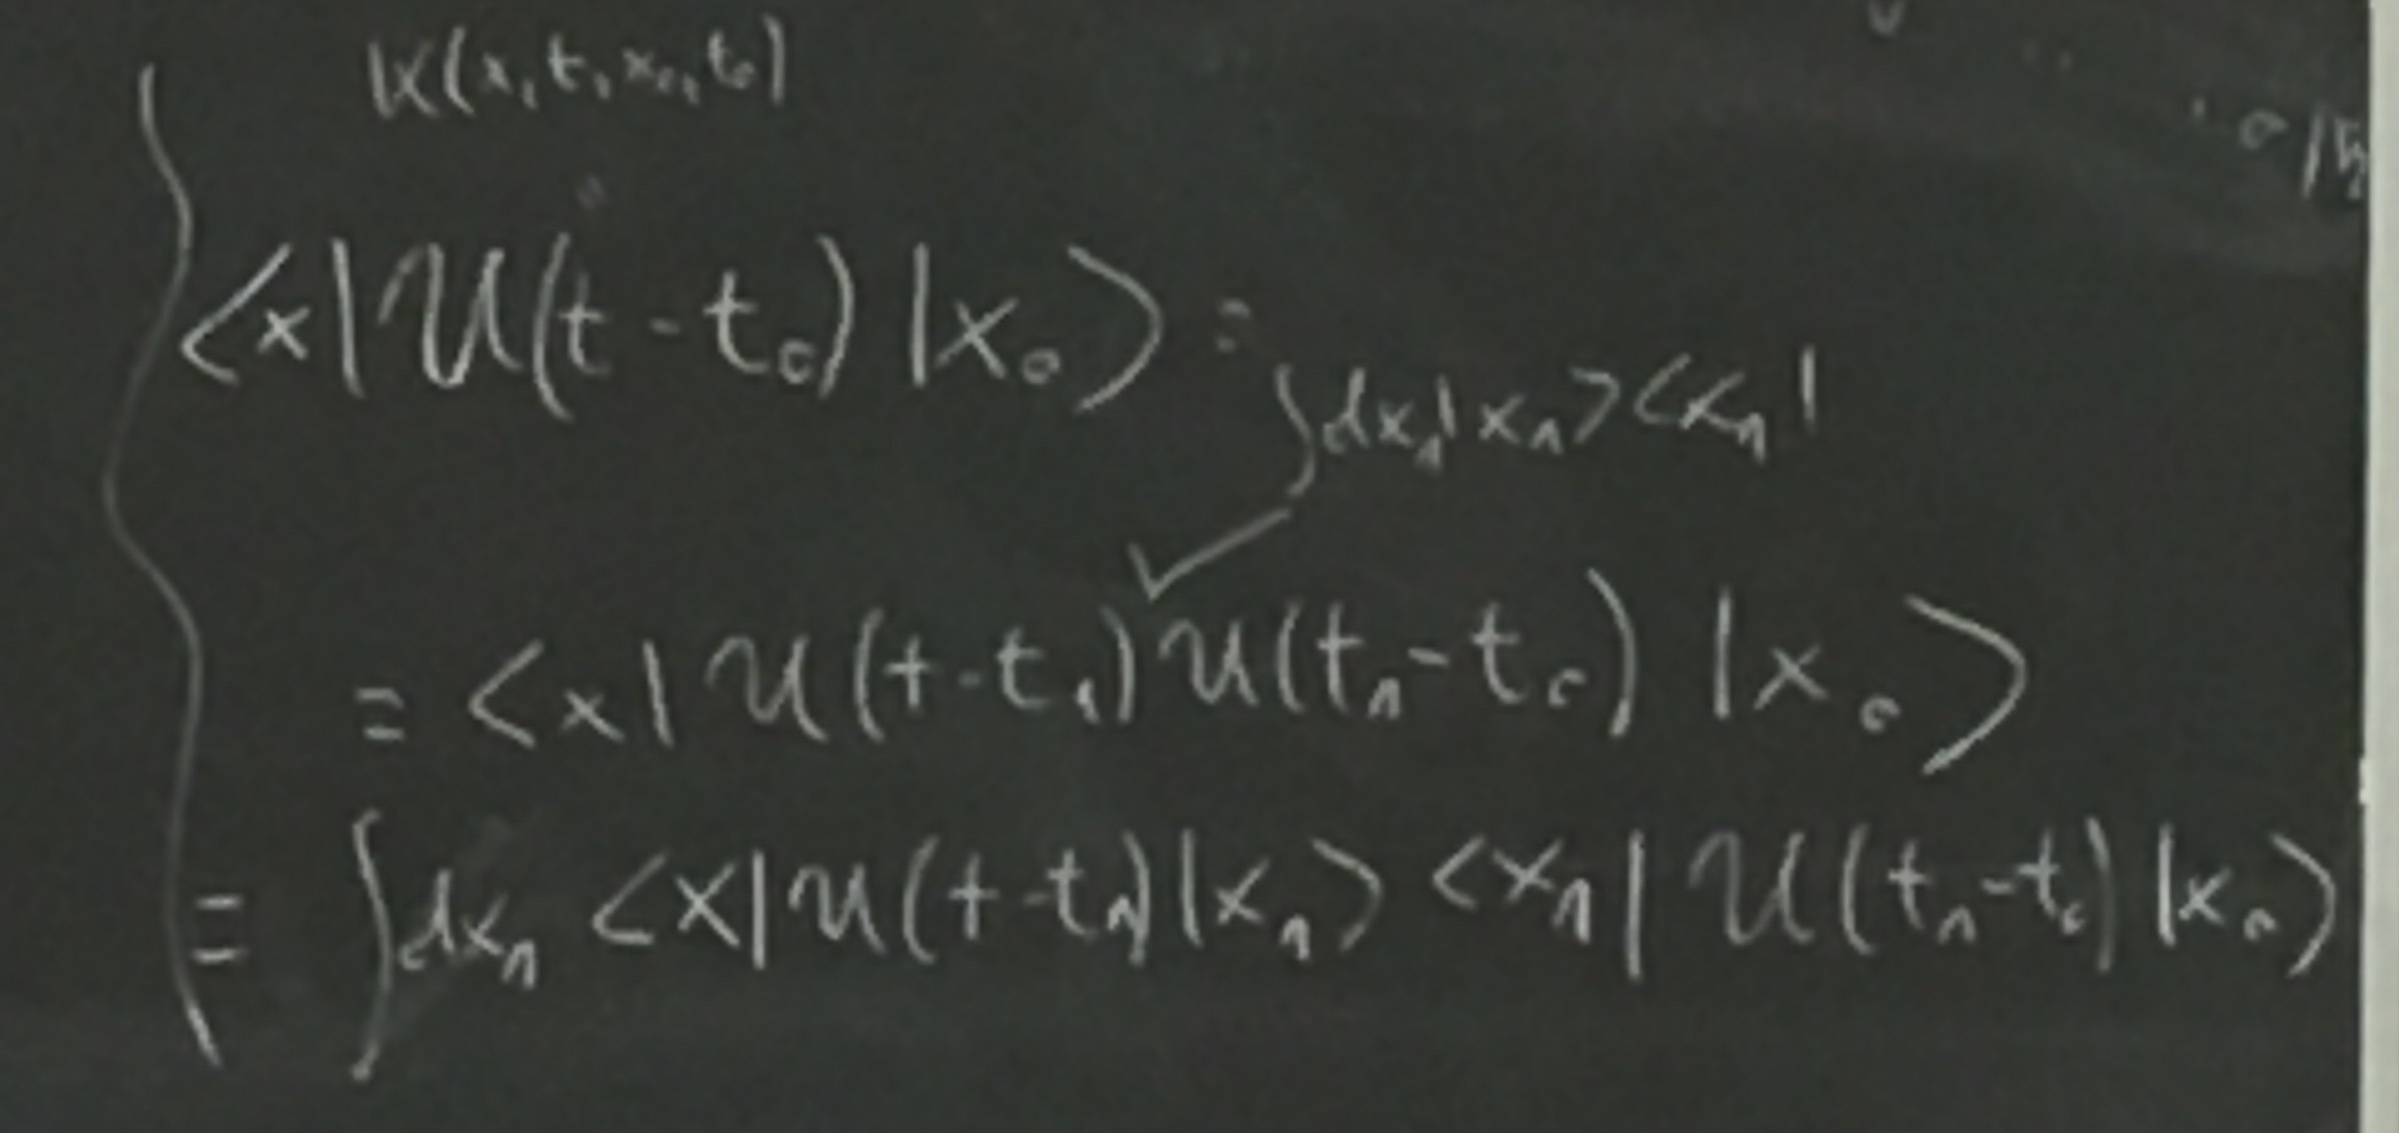
\includegraphics[width=\linewidth]{App_6_Rys_1.JPG}
        \caption{Uzasadnienie dla unitarnego operatora}
        \label{fig:app_6:unitarny}
\end{figure}

\section{Lecture 9}

\begin{figure}[!ht]
        \centering
        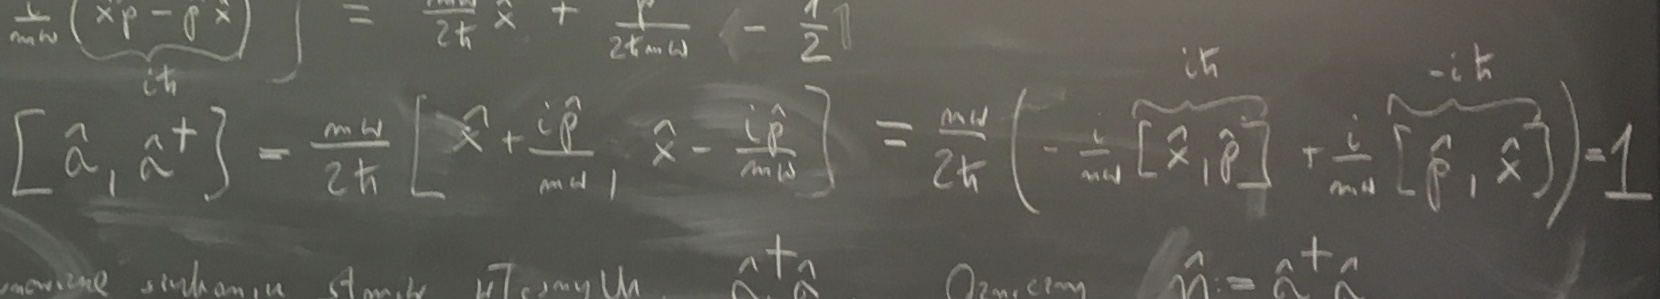
\includegraphics[width=\linewidth]{App_9_Rys_1.JPG}
        \caption{Uzasadnienie dla wartości komutatora $\hat{a}\hat{a}^\dagger$}
        \label{fig:app_9:comm_kreacji_anihillacji}
\end{figure}

\begin{figure}[!ht]
        \centering
        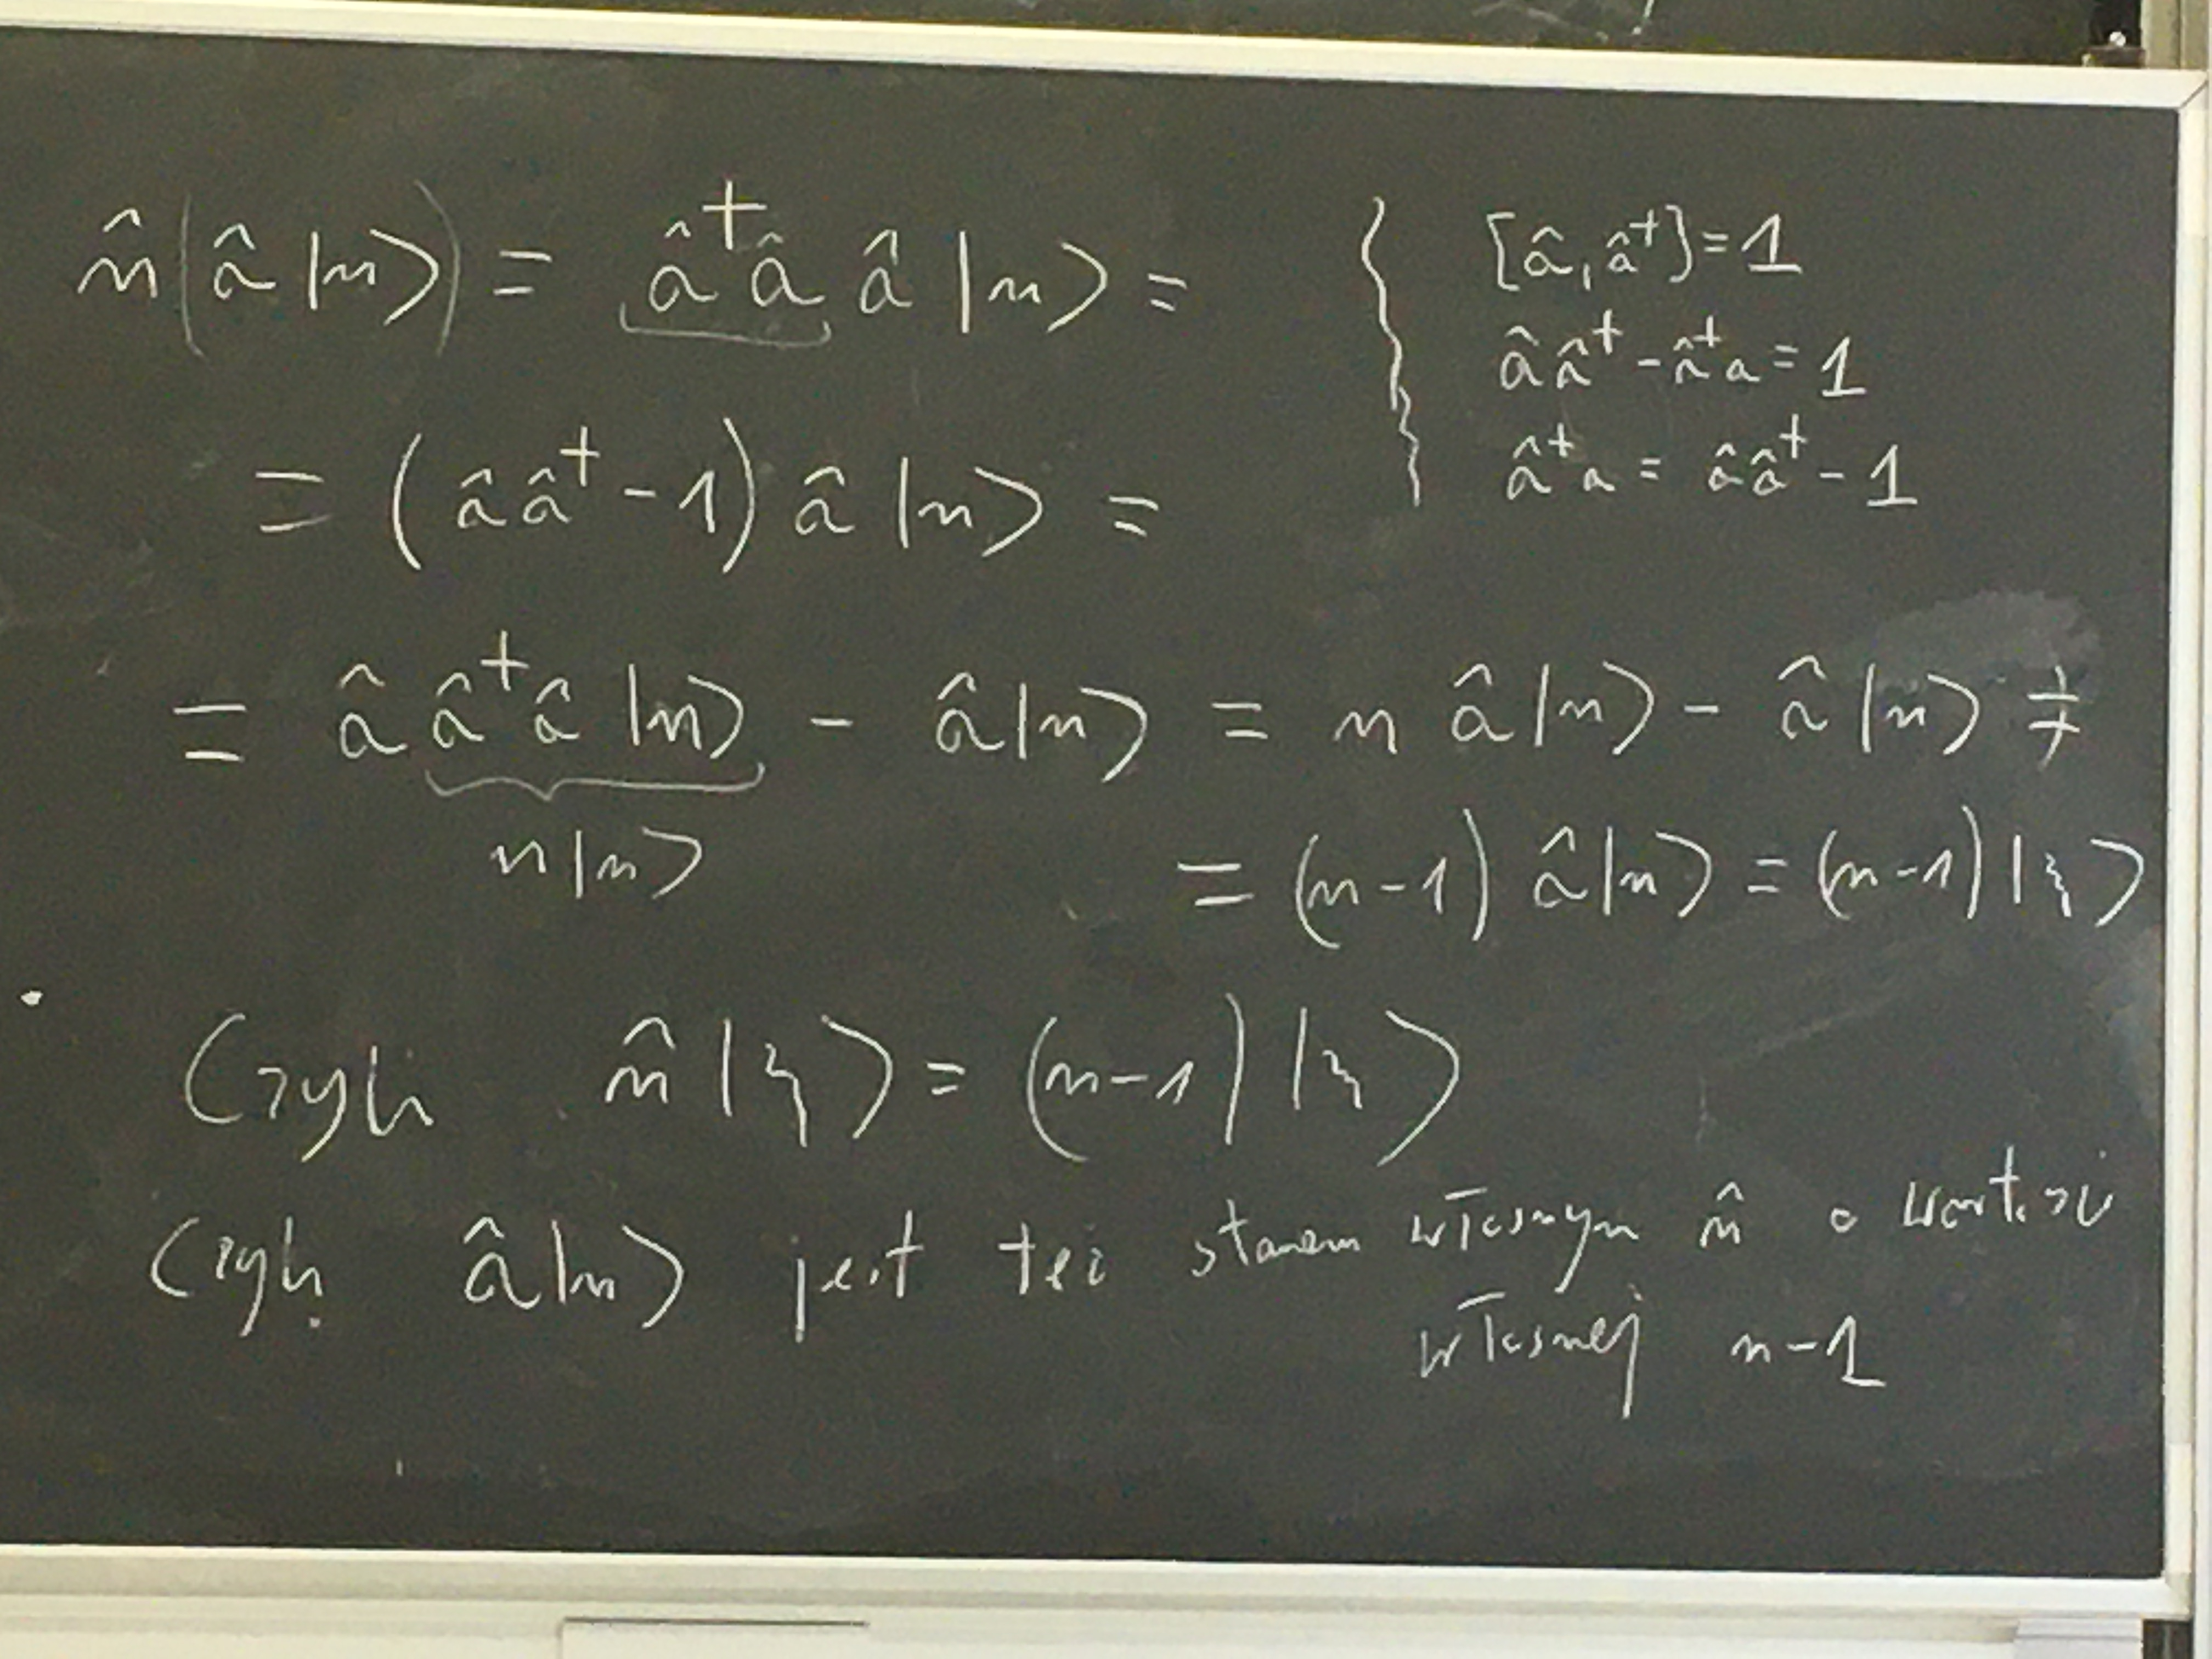
\includegraphics[width=\linewidth]{App_9_Rys_2.JPG}
        \caption{Wyprowadzenie stanu własnego $\hat{n}$}
        \label{fig:app_9:stany_wlasne_n}
\end{figure}


\end{document}